\documentclass{template/openetcs_report}
% Use the option "nocc" if the document is not licensed under Creative Commons
%\documentclass[nocc]{template/openetcs_article}
\usepackage{lipsum,url}
\usepackage{supertabular}
\usepackage{longtable,booktabs}
\usepackage{graphicx}
\usepackage{multirow}
\usepackage{color, colortbl}
\usepackage{hyperref}
\usepackage{listings}
\usepackage{makeidx}
\definecolor{gray}{rgb}{0.8,0.8,0.8}
\usepackage[modulo]{lineno}
\usepackage{float}
\usepackage{fixme}
%\usepackage{pdflscape}
%\usepackage[acronym, % list of acronyms
  %section, % add the glossary to the table of content
            %description,% acronyms have a user-supplied description,
 %style=longheader, % table style
 %nonumberlist % no page number
 %]{glossaries}



\graphicspath{{./template/}{.}{./images/}}

%\renewcommand*{\glspostdescription}{} %Deactivate point at the end of every description
%\renewcommand*{\glossaryname}{Glossary}

%create glossary
% \makeglossaries
 %Glossary terms
% \loadglsentries{glossary}

\begin{document}
\frontmatter
\project{openETCS}

\newcommand{\define}[1]{\index{#1}\emph{#1}}



%Please do not change anything above this line
%============================

% The document metadata is defined below

%assign a report number here
\reportnum{OETCS/WP3/D3.5.2}

%define your workpackage here
\wp{Work Package 3: ``Modeling''}

%set a title here
\title{openETCS Design Specification}

%set a subtitle here
\subtitle{Software Component Design and Internal Interface Specification}

%set the date of the report here
\date{June 2015}


%document approval
%define the name and affiliation of the people involved in the documents approbation here
\creatorname{Peter Mahlmann}
\creatoraffil{DB Netz AG}

\techassessorname{Jan Welte}
\techassessoraffil{Technische Universität Braunschweig}

\qualityassessorname{Izaskun de la Torre}
\qualityassessoraffil{SQS}

\approvalname{Klaus-R\"udiger Hase}
\approvalaffil{DB Netz}


%define a list of authors and their affiliation here

\author{Baseliyos Jacob, Peter Mahlmann, Bernd Hekele, Peyman Farhangi, Stefan Karg, Valerio D´Angelo}
\affiliation{DB Netz AG}

\author{Uwe Steinke}
\affiliation{Siemens AG}

\author{Christian Stahl}
\affiliation{TWT-GmbH}

\author{Jakob Gärtner}
\affiliation{LEA Railergy}

\author{Jos Holtzer, Jan Welvaarts, Vincent Nuhaan}
\affiliation{Nederlands Spoorwegen}

\author{Benjamin Beichler, Thorsten Schulz}
\affiliation{University of Rostock}

\author{Marielle Petit-Doche, Matthias Gudemann}
\affiliation{Systerel}

\author{Vernique Gontier}
\affiliation{All4Tec}

\author{Ghristian Giraud, Fausto Cochetti}
\affiliation{Alstom}

\author{Alexander Stante}
\affiliation{Fraunhofer ESK}




% define the coverart
\coverart[width=350pt]{openETCS_EUPL}

\newpage
%define the type of report
\reporttype{Architecture and Design Specification}


\begin{abstract}
%define an abstract here
This document gives an introduction to the software and component design of the openETCS OBU model. The functional scope is tailored to cover the functionality required for the openETCS demonstration as an objective of the ITEA2 project. The goal is to develop a formal model and to demonstrate the functionality during a proof of concept on the ETCS Level 2 Utrecht Amsterdam track with real scenarios. It has to be read as a complement to the models in SysML and Scade languages. 
\end{abstract}

%=============================
\maketitle

%Modification history
%if you do not need a modification history table for your document simply comment out the eight lines below
%=============================


\chapter*{Modification History}
\tablefirsthead{
\hline 
\rowcolor{gray} 
Version & Section & Modification / Description & Author & Date \\\hline}
\begin{supertabular}{| m{1.2cm} | m{1.5cm} | m{4.0cm} | m{3.5cm} | m{3.5cm} |}
0.1 & Document & Initial document providing structure & Peter Mahlmann& 27.05.2015 \\\hline
0.2 & 2 & New template for design descriptions & Peter Mahlmann& 10.06.2015 \\\hline
\end{supertabular}

% list subsubsections in table of contents
%\setcounter{tocdepth}{3}
\setcounter{secnumdepth}{3}   
\setcounter{tocdepth}{3}   

\tableofcontents
\listoffiguresandtables
\newpage
%=============================

%Uncomment the next line if you need line numbers for tracebility when the document is in review
\linenumbers
%=============================


% The actual document starts below this line
%=============================

\mainmatter


\part{Functional Breakdown}

%set the master document for easy compilation
%!TEX root = ../D3_5_3.tex

\chapter{openETCS API Runtime System and Input to the EVC)}
\label{chp_openETCS_API}
%Authors: Bernd Hekele (DB)

\begin{figure}[hbtp]
\centering
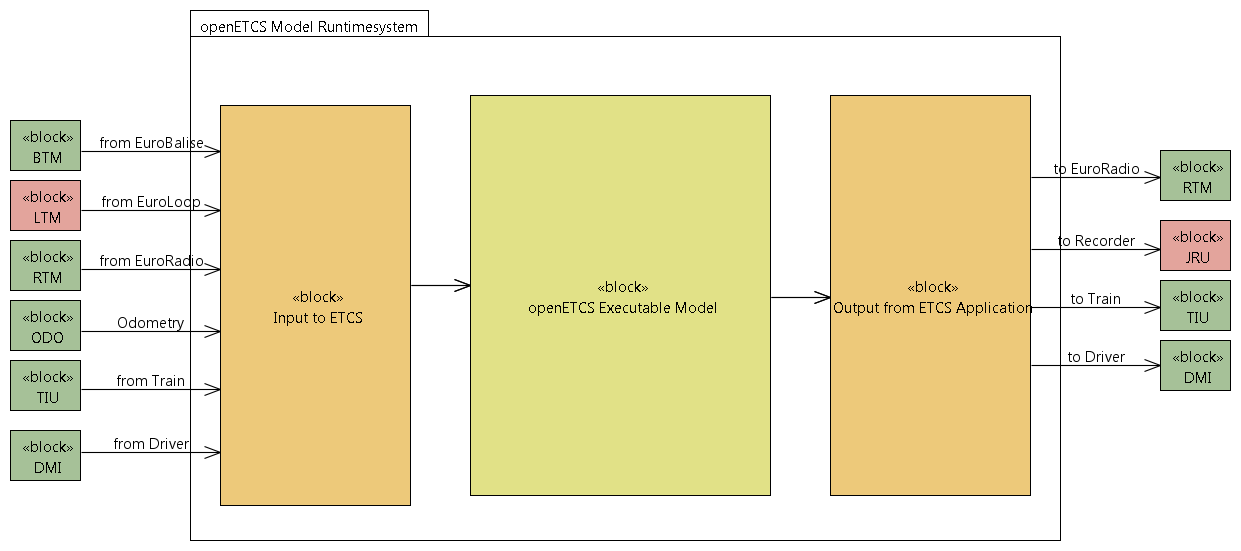
\includegraphics[width=\linewidth]{openETCSAPI.png}
\caption{openETCS API Highlevel View}
\label{fig:apiHighLevel}
\end{figure}

Figure \ref{fig:apiHighLevel} shows the structure of API with respect to the software architecture. Note that red input and output modules are were not yet implemented and thus are not part of the openETCS OBU model. The system covers functions for processing inputs from other units, functions for processing outputs to other functions and a basic runtime system. Inputs are used to feed the input to the executable model before calling it, outputs are used for collecting information provided by the executable model to be passed to the relevant interfaces after the execution cycle has finished.

\section{Principles for Interfaces (openETCS API)}

Information is exchanged via asynchronous \emph{messages}. A message is a set of information corresponding to an event of a particular unit, e.g.~a balise message received from the {BTM}. For possible types of messages please refer to Chapter~\ref{information-flows}.

The information is passed to the executable model as parameters to the synchronous call of a procedure (Interface to the executable model). Since the availability of input messages to the application is not guaranteed the parts of the interfaces are defined with a "present" flag. In addition, fields of input arrays quite often is of variable size. Implementation in the concrete interface in this use-case is the use of a "size" parameter and a "valid"-flag.


\section{openETCS Model Runtime System}
The openETCS model runtime system also provides:
\begin{description}

\item[Input Functions From other Units]
In this entity messages from other connected units are received.

\item[Output Functions to other Units]
The entity writes messages to other connected units.

\item[Conversation Functions for Messages (Bitwalker)]
The conversion function are triggered by Input and Ouput Functions. The main task is to convert input messages from an bit-packed format into logical ETCS messages (the ETCS language) and Output messages from Logical into a bit-packed format. The logical format of the messages is defined for all used types in the openETCS data dictonary.

Variable size elements in the Messages are converted to fixed length arrays with an used elements indicator. Optional elements are indicated with an valid flag.

The conversion routines are responsible for checking the data received is valid. If  faults are detected the information is passed to the openETCS executable model for further reaction. 

\item[Model Cycle]
The version management function is part of the message handling. This implies, conversions from other physical or logical layouts of messages are mapped onto a generic format used in the EVC. Information about the origin version of the message is part of the messages.
 
The executable model is called in cycles. In the cycle 
\begin{itemize}
\item First the received input messages are decoded
\item The input data is passed to the executable model in a predefined order. \textbf{(Details for the interface to be defined)}.
\item Output is encoded according to the {SRS} and passed to the  buffers to the units.
\end{itemize}
\end{description}


\section{Input Interfaces of the openETCS API From other Units of the OBU}
Interfaces are defined in the Scade project APITypes (package API\_Msg\_Pkg.xscade).

In the interfaces the following principles for indicating the quality of the information is used:


\tablefirsthead{
\hline 
\rowcolor{gray} 
Indicator & Type & Purpose \\\hline}
\begin{supertabular}{| p{2 cm} | p{2 cm} | p{8 cm} |}
present & bool & True indicates the component has been changed compared to the previous call of the routine
\\\hline 
valid & bool & True indicates the component is valid to be used. 
\\\hline 
\end{supertabular}

In the next table we can see the interfaces being used in the openETCS system. Details on the interfaces are defined further down.

\tablefirsthead{
\hline 
\rowcolor{gray} 
Unit & Name &  Processing Function  \\\hline}
%\begin{itemize}{| m{1.2cm} | m{1.5cm} | m{1.2cm} | m{3.7cm}  | m{3.7cm} |}
\begin{supertabular}{| c | c | c |}
{BTM} & Balise Telegram & Receive Messages  \\\hline
{DMI} & Driver Machine Interface & DMI Manager  \\\hline
EURORADIO & Communication Management & Communication Management  \\\hline
EURORADIO & Radio Messages & Receive Messages  \\\hline
{ODO} & Odometer & All Parts \\\hline
System TIME & Time system of the OBU & All Parts \\\hline
TIU & Train Data & All Parts \\\hline
\end{supertabular}

Information in the following sections gives an more detailed overview of the structure of the interfaces.


\section{Message based interface (BTM, RTM)}


Balise Message (Track to Train)

\tablefirsthead{
\hline 
\rowcolor{gray} 
Message Name & Optional Packets & Restrictions in the current scope \\\hline}
\begin{supertabular}{| p{4 cm} | p{6 cm} | p{4,5 cm} |}
Balise Telegram &
3: National Values \newline
41: Level Transition Order \newline
42: Session Management  \newline
45: Radio Network registration \newline
46: Conditional Level Transition Order \newline
65: Temporary Speed Restriction \newline
66: Revoke Temporary Speed Restriction \newline
72: Packet for sending plain text messages \newline
137: Stop if in Staff Responsible \newline
255: End of Information \newline
& Used in Scenario
\\\hline
Balise Telegram &
0, 2, 3, 5, 6, 12, 16, 21, 27, 39,
40, 41, 42, 44, 45, 46, 49, 51, 52, 65,
66, 67, 68, 69, 70, 71, 72, 76, 79, 80,
88, 90, 131, 132, 133, 134, 135, 136, 137, 138,
139, 141, 145, 180, 181, 254
&  Not Used in Scenario\\\hline
\end{supertabular}

Radio Messages (Track to Train)

\tablefirsthead{
\hline 
\rowcolor{gray} 
Message Name & Optional Packets & Restrictions in the current scope \\\hline}
\begin{supertabular}{| p{4 cm} | p{6 cm} | p{4,5 cm} |}
2: SR Authorisation & 63:\ List\ of\ Balises\ in\ SR Authority & Message Not Supported \\\hline
3: Movement Authority &
 21:\ Gradient\ Profile\newline
 27: International Static Speed Profile\newline
 49: List of balises for SH Area\newline
 80: Mode profile\newline
 plus common optional packets\newline
 & a \\\hline
9: Request To Shorten MA &
 49: List of balises for SH Area\newline
 80: Mode profile\newline 
& \\\hline
24: General Message &
From RBC:\newline
 21:\ Gradient\ Profile\newline
 27: International Static Speed Profile\newline
 plus common optional packets\newline
From RIU:\newline 44, 45, 143, 180, 254
& Messages from RIU are not supported \\\hline
28: SH authorised & 3, 44, 49
& \\\hline
33: MA with Shifted Location Reference &
 21:\ Gradient\ Profile\newline
 27: International Static Speed Profile\newline
 49: List of balises for SH Area\newline
 80: Mode profile\newline
 plus common optional packets\newline
& \\\hline
37: Infill MA &
5, 21, 27, 39, 40, 41, 44, 49, 51, 52, 65, 66, 68, 69, 70, 71, 80, 88, 138, 139 
 & Message Not Supported \\\hline
List of common optional parameters &
3, 5, 39, 40, 51, 41, 42, 44, 45, 52, 57, 58, 64, 65, 66, 68, 69, 70, 71, 72, 76, 79, 88, 131, 138, 139, 140, 180
& \\\hline
\end{supertabular}

The runtime system is in charge to transfer the messages from its stream mode first to  compressed message format. 

\section{Interfaces to the Time System}
The interface types are defined in the OBU\_Basic\_Types\_Pkg Package. The system time is defined in the basic software.

The system TIME is provided to the executable model at the begin of the cycle. It is not refreshed during the cycle. The time provided to the application is equal to 0 at power-up of the EVC (it is not a “UTC time” nor a “Local
Time”), then must increase at each cycle (unit = 1 msec), until it reaches its maximum value (i.e current EVC
limitation = 24 hours)

\begin{itemize}
\item TIME (T\_internal\_Type, 32-bit INT)\\
Standardized system time type used for all internal time calculations: in ms. The time is defined as a cyclic counter: When the maximum is exceeded the time starts from 0 again. 

\item CLOCK (to be implemented)\\
The clocking system is provided by the JRU. A GPS based clock is assumed to provide the local time.

\end{itemize}

\section{Interfaces to the Odometry System}
The interface types are defined in the OBU\_Basic\_Types\_Pkg Package. 
The odometer gives the current information of the positing system of the train. In this section the structure of the interfaces are only highlighted. Details, including the internal definitions for distances, locations speed and time are implemented in the package. 

\begin{itemize}
\item Odometer (odometry\_T)
\begin{itemize}
\item valid (bool)\\
valid flag, i.e., the information is provided by the ODO system and can be used.
\item timestamp (T\_internal\_Type)\\
of the system when the odometer information was collected. Please, see also general remarks on the time system. 
\item Coordinate (odometryLocation\_T)
\begin{itemize}
\item nominal (L\_internal\_Type) [cm]
\item min (L\_internal\_Type) [cm]
\item max (L\_internal\_Type) [cm]
\end{itemize}
The type used for length values is a 32 bit integer. 
Min and max value give the interval where the train is to be expected. The bounderies are determined by the inaccuracy of the positioning system. All values are set to 0 when the train starts.

\item speed (OdometrySpeeds\_T) [km/h]
\begin{itemize}
\item v\_safeNominal (speed internal type) [km/h]\\
The safe nominal estimation of the speed which will
be bounded between 98\% and 100\% of the upper
estimation
\item v\_rawNominal (speed internal type) [km/h]\\
The raw nominal estimation of the speed which will
be bounded between the lower and the upper
estimations
\item v\_lower (speed internal type) [km/h]\\
The lower estimation of the speed
\item v\_upper (speed internal type) [km/h]\\
The upper estimation of the speed
\end{itemize}
The type used for speed values is a 32 bit integer. 
Min and max value give the interval where the train is to be expected. The bounderies are determined by the inaccuracy of the positioning system. All values are set to 0 when the train starts.
\item acceleration (A\_internal\_Type)[0.01 m/s2],\\
Standardized acceleration type for all internal calculations : in 
\item motionState (Enumeration)\\
indicates whether the train is in motion or in no motion
\item motionDirection (Enumeration)\\
indicates the direction of the train, i.e., CAB-A first, CAB-B first or unknown.
\end{itemize}
\end{itemize}

\section{Interfaces to the Train Interfaces (TIU)}
The following infomration is based on the implementation of the Alstom API. The interface is organised in packets. The packets of the Alstom implementation are listed in the appendix to this document.

The description of interfaces needed for the current scope will be added according to the use.

\section{Output Interfaces of the openETCS API TO other Units of the OBU}

\tablefirsthead{
\hline 
\rowcolor{gray} 
From Function & Name &  To Unit & Description \\\hline}
%\begin{supertabular}{| m{1.2cm} | m{1.5cm} | m{1.2cm} | m{3.7cm}  | m{3.7cm} |}
\begin{supertabular}{| c | c | c | c  | c |}
 & Radio Output Message & \ EURORADIO & \\\hline
 & Communication Management  &  EURORADIO  & \\\hline
 & Driver Information & {DMI} & \\\hline
 & Train Data  & TIU &  
\\\hline
\end{supertabular}

Packets:
to be completed

Radio Messages
to be completed


%-----------------------------------------------------------------------
%\subsection{Runtime- APIl}
%-----------------------------------------------------------------------
%\tbc
%JakobGärtner


\part{Design Description}


\chapter{F1: Receive information from Trackside}

\chapter{F2: ETCS Kernel}
%set the master document for easy compilation
%!TEX root = ../D3_5_2.tex

\section{Manage\_TrackSideInformation\_Integration}

\subsection{Component Requirements}

\todo{Clarify detail f documentation with the trackMessages concept}


\begin{longtable}{p{.25\textwidth}p{.7\textwidth}}
\toprule
Component name			& Manage\_TrackSideInformation\_Integration \\
\midrule
Link to SCADE model		& {\footnotesize \url{https://github.com/openETCS/modeling/blob/master/model/Scade/System/ObuFunctions/ManageLocationRelatedInformation/BaliseGroup/Manage_TrackSideInformation_Integration/Manage_TrackSideInformation_Integration.etp}} \\
\midrule
SCADE designer			& Bernd Hekele, DB Netz AG \\
\midrule
Description				& The block ``Manage\_TrackSideInformation\_Integration'' is responsible for receiving Eurobalise telegrams and Euroradio messages from the API and performs several consistency checks on the inputs.\newline

The block collects the telegrams of balises in order to build balise group messages. Euroradio messages are always delivered as a whole message. On each message, a consistency check is performed, before the data is validated according to the driving direction of the train. In general, messages not designated for the current driving direction of the train are not forwarded to the further processing. After applying consistency checks, the data direction is validated. \\
\midrule
Input documents	& 
See sub-components.\\
\midrule
Safety integrity level		& 4 \\
\midrule
Time constraints		& The component has to be able to receive balise telegrams and radio messages according to the ETCS \cite{subset-41} performance requirements). In highspeed traffic, a group of 8 balises must be read in about 250 msec. In addition, 1 message per sec. on the radio interface is to be expected.\\
\midrule
API requirements 		& Interfaces to this unit are defined in the API sections [BTM], [EURORADIO], [ODO].In these sections, also a detailed definition of the concepts implemented on those interfaces is documented.  \\
\bottomrule
\end{longtable}


\subsection{Interface}

An overview of the interface of component Manage\_TrackSideInformation\_Integration is shown in Figure~\ref{f:receiveAndCheckConsistencyArch}. The inputs and outputs are described in detail in Section~\ref{s:Manage_Trackside_inputs} respectively \ref{s:Manage_Trackside_outputs}. Sub components are described in Section~\ref{s:receivetrackdata_subcomponents}.

\begin{figure}
\center
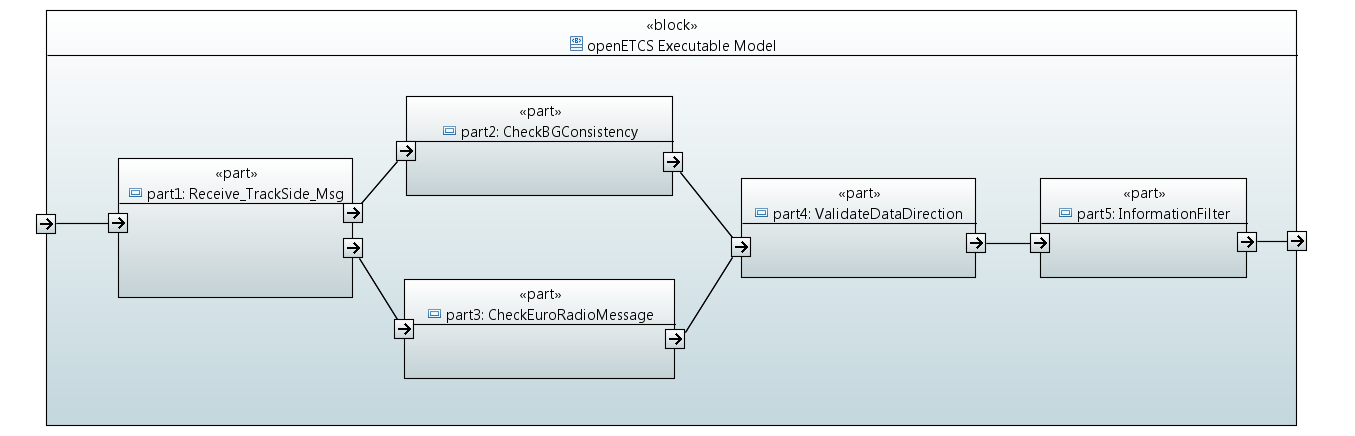
\includegraphics[width=\textwidth]{./images/Input-Messages4.PNG}
\caption{Manage\_TrackSideInformation\_Integration component SysML diagram.}\label{f:receiveAndCheckConsistencyArch}
\end{figure}


\subsubsection{Inputs}\label{s:Manage_Trackside_inputs}

\paragraph{fullChecks}

\begin{longtable}{p{.25\textwidth}p{.7\textwidth}}
\toprule
Input name				& fullChecks \\
\midrule
Description				& Indicates, if all checks on the message should be performed. \\
\midrule
Source					& This item is only relevant in verification phases. In a real system checks are always activated. \\ 
\midrule
Type					& bool \\
\midrule
Valid range of values	& 
\begin{description}
\item[true] All checks are performed.
\item[false] Component InformationFilter is deactivated.
\end{description} \\
\midrule
Behaviour when value is at boundary	& n/a \\
\midrule
Behaviour for values out of valid range	& n/a \\
\midrule
Behaviour when value is erroneous, absent or unwanted (i.e. spurious) & [Description of components behaviour when value is erroneous, absent or unwanted (i.e. spurious)] \\
\bottomrule
\end{longtable}


\paragraph{Receive\_trackSide\_Message}

\begin{longtable}{p{.25\textwidth}p{.7\textwidth}}
\toprule
Input name				& API\_trackSide\_Message \\
\midrule
Description				& Track side message received from the API. The API performs preprocessing of RTM and BTM messages and deliveres a maximum of a single message per cycle. The structure of this message is defined in the API [BTM] and [EURORADIO] sections.\\
\midrule
Source					& API \\ 
\midrule
Type					& API\_Msg\_Pkg::API\_TrackSideInput\_T \\
\midrule
Valid range of values	& [Complete list of valid values] \\
\midrule
Behaviour when value is at boundary	& [Description of components behaviour when input value is at boundary] \\
\midrule
Behaviour for values out of valid range	& [Description of components behaviour when input value is out of valid range] \\
\midrule
Behaviour when value is erroneous, absent or unwanted (i.e. spurious) & [Description of components behaviour when value is erroneous, absent or unwanted (i.e. spurious)] \\
\bottomrule
\end{longtable}


\paragraph{ActualOdometry}

\begin{longtable}{p{.25\textwidth}p{.7\textwidth}}
\toprule
Input name				& ActualOdometry \\
\midrule
Description				& Provided by the external odometry module of the train. It contains relative location information with inaccuracies. \\
\midrule
Source					& Odometer \\ 
\midrule
Type					& Obu\_BasicTypes\_Pkg::odometry\_T \\
\midrule
Valid range of values	& [Complete list of valid values] \\
\midrule
Behaviour when value is at boundary	& [Description of components behaviour when input value is at boundary] \\
\midrule
Behaviour for values out of valid range	& [Description of components behaviour when input value is out of valid range] \\
\midrule
Behaviour when value is erroneous, absent or unwanted (i.e. spurious) & [Description of components behaviour when value is erroneous, absent or unwanted (i.e. spurious)] \\
\bottomrule
\end{longtable}

\paragraph{reset}

\begin{longtable}{p{.25\textwidth}p{.7\textwidth}}
\toprule
Input name				& reset \\
\midrule
Description				& To delete all data stored in the module (e.g.~collected balise telegrams, which do not yet form a complete message), a reset input can be used. If the input is set to true, all data kept in the module is deleted and no input is accepted. \\
\midrule
Source					& Environment \\ 
\midrule
Type					& bool \\
\midrule
Valid range of values	& 
\begin{description}
\item[true] All data kept in the module is deleted and no input is accepted.
\item[false] No action. Data at input is accepted.
\end{description} \\
\midrule
Behaviour when value is at boundary	& [Description of components behaviour when input value is at boundary] \\
\midrule
Behaviour for values out of valid range	& [Description of components behaviour when input value is out of valid range] \\
\midrule
Behaviour when value is erroneous, absent or unwanted (i.e. spurious) & [Description of components behaviour when value is erroneous, absent or unwanted (i.e. spurious)] \\
\bottomrule
\end{longtable}

\paragraph{trainPosition}

\begin{longtable}{p{.25\textwidth}p{.7\textwidth}}
\toprule
Input name				& trainPosition \\
\midrule
Description				& Contains the current position of the train. \\
\midrule
Source					& CalculateTrainPosition \\ 
\midrule
Type					& TrainPosition\_Types\_Pck::trainPosition\_T \\
\midrule
Valid range of values	& \\
\midrule
Behaviour when value is at boundary	& [Description of components behaviour when input value is at boundary] \\
\midrule
Behaviour for values out of valid range	& [Description of components behaviour when input value is out of valid range] \\
\midrule
Behaviour when value is erroneous, absent or unwanted (i.e. spurious) & [Description of components behaviour when value is erroneous, absent or unwanted (i.e. spurious)] \\
\bottomrule
\end{longtable}

\paragraph{modeAndLevel}

\begin{longtable}{p{.25\textwidth}p{.7\textwidth}}
\toprule
Input name				& modeAndLevel \\
\midrule
Description				& Provides the current level and mode of the EVC. \\
\midrule
Source					& ModeAndLevel \\ 
\midrule
Type					& BG\_Types\_Pkg::ModeAndLevelStatus\_T \\
\midrule
Valid range of values	& [Complete list of valid values] \\
\midrule
Behaviour when value is at boundary	& [Description of components behaviour when input value is at boundary] \\
\midrule
Behaviour for values out of valid range	& [Description of components behaviour when input value is out of valid range] \\
\midrule
Behaviour when value is erroneous, absent or unwanted (i.e. spurious) & [Description of components behaviour when value is erroneous, absent or unwanted (i.e. spurious)] \\
\bottomrule
\end{longtable}


\paragraph{tNvContact}

\begin{longtable}{p{.25\textwidth}p{.7\textwidth}}
\toprule
Input name				& tNvContact \\
\midrule
Description				& For monitoring the safe radio connection, this national value is needed as an input. \\
\midrule
Source					& Database \\ 
\midrule
Type					& Obu\_BasicTypes\_Pkg::T\_internal\_Type \\
\midrule
Valid range of values	& [Complete list of valid values] \\
\midrule
Behaviour when value is at boundary	& [Description of components behaviour when input value is at boundary] \\
\midrule
Behaviour for values out of valid range	& [Description of components behaviour when input value is out of valid range] \\
\midrule
Behaviour when value is erroneous, absent or unwanted (i.e. spurious) & [Description of components behaviour when value is erroneous, absent or unwanted (i.e. spurious)] \\
\bottomrule
\end{longtable}


\paragraph{lastRelevantEventTimestamp}

\begin{longtable}{p{.25\textwidth}p{.7\textwidth}}
\toprule
Input name				& lastRelevantEventTimestamp \\
\midrule
Description				& For monitoring the safe radio connection, it is necessary that the time between two packets is less than the value of {T\_NVCONTACT}.\newline
In situations like level-changes or announced radio holes, not the timestamp of the last message is relevant for comparison, but the timestamp of the last relevant event. This can for example be the timestamp of the level change or the timestamp of the moment, when the train was passing the end of the radiohole.\newline
For performing this check, the timestamp of the last relevant event is provided to the model as an {T\_internal\_Type}-type. \\
\midrule
Source					& Database \\ 
\midrule
Type					& Obu\_BasicTypes\_Pkg::T\_internal\_Type \\
\midrule
Valid range of values	& [Complete list of valid values] \\
\midrule
Behaviour when value is at boundary	& [Description of components behaviour when input value is at boundary] \\
\midrule
Behaviour for values out of valid range	& [Description of components behaviour when input value is out of valid range] \\
\midrule
Behaviour when value is erroneous, absent or unwanted (i.e. spurious) & [Description of components behaviour when value is erroneous, absent or unwanted (i.e. spurious)] \\
\bottomrule
\end{longtable}


\paragraph{connectionStatus}

\begin{longtable}{p{.25\textwidth}p{.7\textwidth}}
\toprule
Input name				& connectionStatus \\
\midrule
Description				& Status information about the radio connection. The information is needed to perform the timing check, which depends on the connection state. \\
\midrule
Source					& ManageRadioCommunication \\ 
\midrule
Type					& Radio\_Types\_Pkg::sessionStatus\_Type \\
\midrule
Valid range of values	& 
\begin{description}
\item[DISCONNECTED] The OBU is currently not connected to a RBC.
\item[CONNECTING] The OBU is currently connecting to the RBC. Received messages belong to the process of establishing a connection.
\item[CONNECTION\_ESTABLISHED] The connection to the RBC is established.
\end{description} \\
\midrule
Behaviour when value is at boundary	& [Description of components behaviour when input value is at boundary] \\
\midrule
Behaviour for values out of valid range	& [Description of components behaviour when input value is out of valid range] \\
\midrule
Behaviour when value is erroneous, absent or unwanted (i.e. spurious) & [Description of components behaviour when value is erroneous, absent or unwanted (i.e. spurious)] \\
\bottomrule
\end{longtable}


\paragraph{inSupervisingRbcId}

\begin{longtable}{p{.25\textwidth}p{.7\textwidth}}
\toprule
Input name				& inSupervisingRbcId \\
\midrule
Description				& For the sub component InformationFilter, the information which radio messages are sent by the supervising RBC is needed. To recognize these messages, the identifier of the supervising RBC is needed. \\
\midrule
Source					& Database \\ 
\midrule
Type					& int \\
\midrule
Valid range of values	& [Complete list of valid values] \\
\midrule
Behaviour when value is at boundary	& [Description of components behaviour when input value is at boundary] \\
\midrule
Behaviour for values out of valid range	& [Description of components behaviour when input value is out of valid range] \\
\midrule
Behaviour when value is erroneous, absent or unwanted (i.e. spurious) & [Description of components behaviour when value is erroneous, absent or unwanted (i.e. spurious)] \\
\bottomrule
\end{longtable}


\paragraph{inAnnouncedBGs}

\begin{longtable}{p{.25\textwidth}p{.7\textwidth}}
\toprule
Input name				& inAnnouncedBGs \\
\midrule
Description				& Provides information about balise groups which will be passed by the train soon. This information is generated by Calculate Train Position based on the linking information received from trackside. \\
\midrule
Source					& CalculateTrainPosition \\ 
\midrule
Type					& TrainPosition\_Types\_Pck::positionedBGs\_T \\
\midrule
Valid range of values	& [Complete list of valid values] \\
\midrule
Behaviour when value is at boundary	& [Description of components behaviour when input value is at boundary] \\
\midrule
Behaviour for values out of valid range	& [Description of components behaviour when input value is out of valid range] \\
\midrule
Behaviour when value is erroneous, absent or unwanted (i.e. spurious) & [Description of components behaviour when value is erroneous, absent or unwanted (i.e. spurious)] \\
\bottomrule
\end{longtable}


\paragraph{q\_nvlocacc}

\begin{longtable}{p{.25\textwidth}p{.7\textwidth}}
\toprule
Input name				& q\_nvlocacc \\
\midrule
Description				& The national value determines the location accuracy. \\
\midrule
Source					& Database \\ 
\midrule
Type					& Q\_NVLOCACC \\
\midrule
Valid range of values	& [Complete list of valid values] \\
\midrule
Behaviour when value is at boundary	& [Description of components behaviour when input value is at boundary] \\
\midrule
Behaviour for values out of valid range	& [Description of components behaviour when input value is out of valid range] \\
\midrule
Behaviour when value is erroneous, absent or unwanted (i.e. spurious) & [Description of components behaviour when value is erroneous, absent or unwanted (i.e. spurious)] \\
\bottomrule
\end{longtable}



\subsubsection{Outputs}\label{s:Manage_Trackside_outputs}

\paragraph{outputMessage}

\begin{longtable}{p{.25\textwidth}p{.7\textwidth}}
\toprule
Output name				& outputMessage \\
\midrule
Description				& Combines both balise and radio messages to one common datatype. This datatype contains all variables and packets, which are possible for the given scenario. \\
\midrule
Destination				& [Name of the destination component(s)] \\ 
\midrule
Type					& Common\_Types\_Pkg::ReceivedMessage\_T \\
\midrule
Valid range of values	& [Complete list of valid values] \\
\midrule
Behaviour when value is at boundary	& [Description of components behaviour when output value is at boundary] \\
\midrule
Behaviour for values out of valid range	& [Description of components behaviour when output value is out of valid range] \\
\midrule
Behaviour when value is erroneous, absent or unwanted (i.e. spurious) & [Description of components behaviour when value is erroneous, absent or unwanted (i.e. spurious)] \\
\bottomrule
\end{longtable}


\paragraph{ApplyServiceBrake}

\begin{longtable}{p{.25\textwidth}p{.7\textwidth}}
\toprule
Output name				& ApplyServiceBrake \\
\midrule
Description				&  Indicates if the balise group the train just passed could not be processed correctly. The check results in the request for a service break. \\
\midrule
Destination				& [Name of the destination component(s)] \\ 
\midrule
Type					& bool \\
\midrule
Valid range of values	& [Complete list of valid values] \\
\midrule
Behaviour when value is at boundary	& [Description of components behaviour when output value is at boundary] \\
\midrule
Behaviour for values out of valid range	& [Description of components behaviour when output value is out of valid range] \\
\midrule
Behaviour when value is erroneous, absent or unwanted (i.e. spurious) & [Description of components behaviour when value is erroneous, absent or unwanted (i.e. spurious)] \\
\bottomrule
\end{longtable}


\paragraph{BadBaliseMessageToDMI}

\begin{longtable}{p{.25\textwidth}p{.7\textwidth}}
\toprule
Output name				& BadBaliseMessageToDMI \\
\midrule
Description				& Information to be passed to the DMI to indicate the reception of a ``bad balise'' to the driver. \\
\midrule
Destination				& DMI \\ 
\midrule
Type					& bool \\
\midrule
Valid range of values	& \begin{description}
\item[true] ???
\item[false] ???
\end{description} \\
\midrule
Behaviour when value is at boundary	& [Description of components behaviour when output value is at boundary] \\
\midrule
Behaviour for values out of valid range	& [Description of components behaviour when output value is out of valid range] \\
\midrule
Behaviour when value is erroneous, absent or unwanted (i.e. spurious) & [Description of components behaviour when value is erroneous, absent or unwanted (i.e. spurious)] \\
\bottomrule
\end{longtable}


\paragraph{errorLinkedBG}

\begin{longtable}{p{.25\textwidth}p{.7\textwidth}}
\toprule
Output name				& errorLinkedBG \\
\midrule
Description				& [Brief description of the output] \\
\midrule
Destination				& [Name of the destination component(s)] \\ 
\midrule
Type					& [Type of the output] \\
\midrule
Valid range of values	& \begin{description}
\item[true] An error in a linked balise group was detected.
\item[false] No error in a linked balise group was detected.
\end{description} \\
\midrule
Behaviour when value is at boundary	& [Description of components behaviour when output value is at boundary] \\
\midrule
Behaviour for values out of valid range	& [Description of components behaviour when output value is out of valid range] \\
\midrule
Behaviour when value is erroneous, absent or unwanted (i.e. spurious) & [Description of components behaviour when value is erroneous, absent or unwanted (i.e. spurious)] \\
\bottomrule
\end{longtable}


\paragraph{errorUnlinkedBG}

\begin{longtable}{p{.25\textwidth}p{.7\textwidth}}
\toprule
Output name				& errorUnlinkedBG \\
\midrule
Description				& [Brief description of the output] \\
\midrule
Destination				& [Name of the destination component(s)] \\ 
\midrule
Type					& bool \\
\midrule
Valid range of values	& \begin{description}
\item[true] An error in a unlinked balise group was detected.
\item[false] No error in a unlinked balise group was detected.
\end{description} \\
\midrule
Behaviour when value is at boundary	& [Description of components behaviour when output value is at boundary] \\
\midrule
Behaviour for values out of valid range	& [Description of components behaviour when output value is out of valid range] \\
\midrule
Behaviour when value is erroneous, absent or unwanted (i.e. spurious) & [Description of components behaviour when value is erroneous, absent or unwanted (i.e. spurious)] \\
\bottomrule
\end{longtable}

\paragraph{passedBG}

\begin{longtable}{p{.25\textwidth}p{.7\textwidth}}
\toprule
Output name				& passedBG \\
\midrule
Description				& Provides the received balise group message in a special format needed by the component CalculateTrainPosition. \\
\midrule
Destination				& [Name of the destination component(s)] \\ 
\midrule
Type					& BG\_Types\_Pkg::passedBG\_T \\
\midrule
Valid range of values	& [Complete list of valid values] \\
\midrule
Behaviour when value is at boundary	& [Description of components behaviour when output value is at boundary] \\
\midrule
Behaviour for values out of valid range	& [Description of components behaviour when output value is out of valid range] \\
\midrule
Behaviour when value is erroneous, absent or unwanted (i.e. spurious) & [Description of components behaviour when value is erroneous, absent or unwanted (i.e. spurious)] \\
\bottomrule
\end{longtable}


\paragraph{outPositionParams}

\begin{longtable}{p{.25\textwidth}p{.7\textwidth}}
\toprule
Output name				& outPositionParams \\
\midrule
Description				& Provides the parameters for the position report in a special format needed by the component ProvidePositionReport. \\
\midrule
Destination				& [Name of the destination component(s)] \\ 
\midrule
Type					& Common\_Types\_Pkg::PositionReportParameter\_T \\
\midrule
Valid range of values	& [Complete list of valid values] \\
\midrule
Behaviour when value is at boundary	& [Description of components behaviour when output value is at boundary] \\
\midrule
Behaviour for values out of valid range	& [Description of components behaviour when output value is out of valid range] \\
\midrule
Behaviour when value is erroneous, absent or unwanted (i.e. spurious) & [Description of components behaviour when value is erroneous, absent or unwanted (i.e. spurious)] \\
\bottomrule
\end{longtable}


\paragraph{outRadioManagement}

\begin{longtable}{p{.25\textwidth}p{.7\textwidth}}
\toprule
Output name				& outRadioManagement \\
\midrule
Description				& Provides the messages for radio session management in a special format needed by the component ManagementOfRadioCommunication. \\
\midrule
Destination				& [Name of the destination component(s)] \\ 
\midrule
Type					& Common\_Types\_Pkg::radioManagementMessage\_T \\
\midrule
Valid range of values	& [Complete list of valid values] \\
\midrule
Behaviour when value is at boundary	& [Description of components behaviour when output value is at boundary] \\
\midrule
Behaviour for values out of valid range	& [Description of components behaviour when output value is out of valid range] \\
\midrule
Behaviour when value is erroneous, absent or unwanted (i.e. spurious) & [Description of components behaviour when value is erroneous, absent or unwanted (i.e. spurious)] \\
\bottomrule
\end{longtable}


\paragraph{radioSequenceError}

\begin{longtable}{p{.25\textwidth}p{.7\textwidth}}
\toprule
Output name				& radioSequenceError \\
\midrule
Description				& [Brief description of the output] \\
\midrule
Destination				& [Name of the destination component(s)] \\ 
\midrule
Type					& bool \\
\midrule
Valid range of values	& \begin{description}
\item[true] A sequence error or a timeout has been detected in the radio message.
\item[false] No error in the radio message sequence was detected.
\end{description} \\
\midrule
Behaviour when value is at boundary	& [Description of components behaviour when output value is at boundary] \\
\midrule
Behaviour for values out of valid range	& [Description of components behaviour when output value is out of valid range] \\
\midrule
Behaviour when value is erroneous, absent or unwanted (i.e. spurious) & [Description of components behaviour when value is erroneous, absent or unwanted (i.e. spurious)] \\
\bottomrule
\end{longtable}


\paragraph{radioMessageConsistencyError}

\begin{longtable}{p{.25\textwidth}p{.7\textwidth}}
\toprule
Output name				& radioMessageConsistencyError \\
\midrule
Description				& [Brief description of the output] \\
\midrule
Destination				& [Name of the destination component(s)] \\ 
\midrule
Type					& bool \\
\midrule
Valid range of values	& \begin{description}
\item[true] A consistency error has been detected in the radio message.
\item[false] No consistency error in the radio message was detected.
\end{description} \\
\midrule
Behaviour when value is at boundary	& [Description of components behaviour when output value is at boundary] \\
\midrule
Behaviour for values out of valid range	& [Description of components behaviour when output value is out of valid range] \\
\midrule
Behaviour when value is erroneous, absent or unwanted (i.e. spurious) & [Description of components behaviour when value is erroneous, absent or unwanted (i.e. spurious)] \\
\bottomrule
\end{longtable}


% Description of sub components
\subsection{Sub Components}\label{s:receivetrackdata_subcomponents}

\subsubsection{Receive\_TrackSide\_Msg}
%set the master document for easy compilation
%!TEX root = ../D3_5_3.tex

\todo[inline]{Responsible developer has to be identified.}
\paragraph{Component Requirements}
\begin{longtable}{p{.25\textwidth}p{.7\textwidth}}
\toprule
Component name			& Receive\_TrackSide\_Msg \\
\midrule
Link to SCADE model		& {\footnotesize \url{https://github.com/openETCS/modeling/tree/master/model/Scade/System/ObuFunctions/ManageLocationRelatedInformation/BaliseGroup/Receive_TrackSide_Msg}} \\
\midrule
SCADE designer			& [Name, affiliation] \\
\midrule
Description				& This function defines the interface of the OBU model to the openETCS generic API for Eurobalise  and Euroradio messages. On the interface, either a valid telegram/message is provided or a telegram/message is indicated which could not be received correct when passing the balise or receiving the radio message. The function passes a balise telegram without major changes of the information to the next entity for collecting the balise group information. This entity collects telegrams received via the interface into Balise Group Information. In case of a radio message, the message is converted to an internal format for further processing and passed without changing the information contained.
\begin{itemize}
\item The decoding of balises is done at the API. Also, packets received via the interface are already transformed into a usable shape.
\item Only packets used inside the current model are passed via the interface.
\item Treatment of Packet 5: Linking Information.
Linking Information is added to the linking array starting from index 0 without gaps. Used elements are marked as valid. Elements are sorted according to the order given by the telegram sequence.
\item Telegrams received as invalid are passed to the ``Check-Function'' to process errors in communication with the track side according to the requirements and in a single place.
Telegrams are added to the telegram array starting from index 0 without gaps. Used elements are marked as valid. Elements are stored according to the order given by the telegram sequence.
\item This function does not process information from the packets. The information is passed to the check without further processing of the values. 
\end{itemize} \\
\midrule
Input documents	&
  Subset-026, Chapter 7 and 8: Definition of the Balise Telegram\newline
  Subset-026, Chapter 4.2.2, 4.2.4, 4.2.9: Interface to the BTM\newline
  Subset-026, Chapter 3.4.1 - 3.4.3, 3.16.2: Handling of Balise Telegrams\newline
  Subset-026, Chapter 3.16.2: Check of the balise group\newline
  Subset-026, Chapter 3.4.2: Determining the orientation\newline
  Subset-026, Chapter 4.5.2 Active Functions Table\newline
  Subset-026, Chapter 8.4.4: Rules for Euroradio messages \\
\midrule
Safety integrity level		& 4 \\
\midrule
Time constraints		& n/a \\
\midrule
API requirements 		& n/a \\
\bottomrule
\end{longtable}


\paragraph{Interface}

For an overview of the interface of this internal component we refer to the SCADE model (cf.~link above) respectively the SCADE generated documentation.

\subsubsection{CheckBGConsistency}
%set the master document for easy compilation
%!TEX root = ../D3_5_3.tex

\paragraph{Component Requirements}

\begin{longtable}{p{.25\textwidth}p{.7\textwidth}}
\toprule
Component name			& CheckBGConsistency \\
\midrule
Link to SCADE model		& {\footnotesize \url{https://github.com/openETCS/modeling/tree/master/model/Scade/System/ObuFunctions/ManageLocationRelatedInformation/BaliseGroup/CheckBGConsistency}} \\
\midrule
SCADE designer			& [Name, affiliation] \\
\midrule
Description				& This function verifies the completeness and correctness of the received messages from balise groups. A message consists of at least a telegram and a maximum of 8 telegrams.
\begin{itemize}
\item A message is still complete and correct, if a telegram is missing (or not decoded or incomplete decoded ), and this telegram is duplicated within the balise group and the duplicating one is correctly read.
\item By more than one telegram, the order of the telegrams must be either ascending (nominal) or descending(reverse).
\item A message is correct, if  all message counters (M MCUNT) do not equal 254 (that means: The telegram never fits any message of the group). A message counter can be equal 255 (that means: The telegram fits with all telegrams of the same balise group) and all other values must be the same.
\end{itemize}
The orientation of the BG will also be calculated in this block. The check, if the message has been received in due time and the right at the right expected location, will be performed in "Calculate Train Position". The checks on the validity of the data in the packets and the validity with respect to the direction of motion will be performed in other modules, e.g. "Validate Data Direction". \\
\midrule
Input documents	& 
Subset-026, Chapter 7 and 8: Definition of the Balise Telegram\newline
Subset-026, Chapter 3.4.1-3, 3.16.2: Handling of Balise Telegrams\newline
Subset-026, Chapter 3.16.2: Check of the balise group\newline
Subset-026, Chapter 4.5.2: Active Functions Table\\
\midrule
Safety integrity level		& 4 \\
\midrule
Time constraints		& n/a \\
\midrule
API requirements 		& n/a \\
\bottomrule
\end{longtable}


\paragraph{Interface}

For an overview of the interface of this internal component we refer to the SCADE model (c.f.~link above) respectively the SCADE generated documentation.

\subsubsection{CheckEuroradioMessage}
%set the master document for easy compilation
%!TEX root = ../D3_5_3.tex

\paragraph{Component Requirements}

\begin{longtable}{p{.25\textwidth}p{.7\textwidth}}
\toprule
Component name			& CheckEuroradioMessage \\
\midrule
Link to SCADE model		& {\footnotesize \url{https://github.com/openETCS/modeling/tree/b9c31ce6fdf702b412bbeab3032a8a4dc7c92e5c/model/Scade/System/ObuFunctions/ManageLocationRelatedInformation/BaliseGroup/CheckEuroRadioMessage}} \\
\midrule
SCADE designer			& Stefan Karg, LEA Railergy \\
\midrule
Description				& The component ``CheckEuroradioMessage'' performs consistency and timing checks on the received radio message. These checks are:
\begin{itemize}
 \item Checking the message sequence.
 \item Check if the message violates timing constraints (T\_NVCONTACT).
 \item Check if all mandatory elements are included.
 \item Check if no elements are included, which are forbidden for the given message id.
\end{itemize}
Messages, which violate one or more of these criteria are marked as invalid in the message header and the component signals the reason for the invalidation via different flags as described in the SCADE model. \\
\midrule
Input documents	& 
  Subset-026, Chapter 3.16\newline
  Subset-026, Chapter 8.4.4\\
\midrule
Safety integrity level		& 4 \\
\midrule
Time constraints		& n/a \\
\midrule
API requirements 		& n/a \\
\bottomrule
\end{longtable}


\paragraph{Interface}

For an overview of the interface of this internal component we refer to the SCADE model (cf.~link above) respectively the SCADE generated documentation.

\subsubsection{ValidateDataDirection}
%set the master document for easy compilation
%!TEX root = ../D3_5_3.tex

\paragraph{Component Requirements}

\begin{longtable}{p{.25\textwidth}p{.7\textwidth}}
\toprule
Component name			& CheckEuroradioMessage \\
\midrule
Link to SCADE model		& {\footnotesize \url{https://github.com/openETCS/modeling/tree/master/model/Scade/System/ObuFunctions/ManageLocationRelatedInformation/BaliseGroup/ValidateDataDirection}} \\
\midrule
SCADE designer			& ??? \\
\midrule
Description				& The component filters an input message in order to mark all elements as invalid, which are not designated for the current driving direction of the train.
\begin{itemize}
 \item The operator contains two processing paths for different message types. Radio messages and balise group messages are handeled in a different way. For validating the data direction of a radio message, the check is performed using the balise group referenced in the radio message header as relevant balise group. For balise group message, the LRBG is used.
 \item The metadata of packets, which are recognized as not valid for the current driving direction, is invalidated.
\end{itemize} \\
\midrule
Input documents	& 
  Subset-026, Chapter 3.6.3 \\
\midrule
Safety integrity level	& 4 \\
\midrule
Time constraints		& n/a \\
\midrule
API requirements 		& n/a \\
\bottomrule
\end{longtable}


\paragraph{Interface}

For an overview of the interface of this internal component we refer to the SCADE model (c.f.~link above) respectively the SCADE generated documentation.

\subsubsection{InformationFilter}
%set the master document for easy compilation
%!TEX root = ../D3_5_3.tex

\paragraph{Component Requirements}

\todo[inline]{Information filter component description needs to be checked, i.e. is the description still up to date? Should more documentation provided for this component in the ADD (please check with Bernd Hekele)?}
\begin{longtable}{p{.25\textwidth}p{.7\textwidth}}
\toprule
Component name			& CheckEuroradioMessage \\
\midrule
Link to SCADE model		& {\footnotesize \url{https://github.com/openETCS/modeling/tree/master/model/Scade/System/ObuFunctions/ManageLocationRelatedInformation/BaliseGroup/InformationFilter}} \\
\midrule
SCADE designer			& Christian Stahl, TWT\newline
Alexander Stante, FhG \\
\midrule
Description				& The filter receives track information (balise and radio) and filters them depending of the mode, level and source of the message. Only messages that pass the filter are valid and should be considered by other ETCS subsystems. Figure~\ref{fig:InformationFilterHighLevel} shows the high\-level decomposition of the functionality. The filter is consists of four  components: FirstFilter, SecondFilter, ThirdFilter and TransitionBuffer.

\begin{description}
\item[FirstFilter] This filter performs filtering of messages
based on the current ETCS level. The decisions taken process is
described via a big decision table which contains rows for every
packet and columns for every ETCS level. This table encodes also if
certain additional information is necessary to filter a message like
pending ETCS Level transitions. Based on this filter packets of an
incoming message is either rejected, accepted or the whole message is
put in the TransitionBuffer. Messages are put in the TransitionBuffer
if there is an announced level transition and the received message is
only valid for the upcoming level.

\item[SecondFilter] The SecondFilter mainly considers messages
that are received via Euroradio. Certain messages are directly
rejected while other may be stored in the TransitionBuffer. The buffer
is used to store messages that are received from non supervising RBCs,
but will be reevaluated after a RBC transition.

\item[ThirdFilter] The last filter is functionally very similiar
the the FirstFilter, however it filters depending on the mode. It also
contains a decision table with rows for every packet but the columns
are modes.

\item[TransitionBuffer] The InformationFilter uses two
TransitionBuffers. One is used to store up to three messages for the
ETCS level transition and the other buffer is used for RBC
transitions. The buffer is designed as a ring buffer and message are
read in FIFO order.
\end{description} \\
\midrule
Input documents	& 
  Subset-026, Chapter 4.8 \\
\midrule
Safety integrity level	& 4 \\
\midrule
Time constraints		& n/a \\
\midrule
API requirements 		& n/a \\
\bottomrule
\end{longtable}

\begin{figure}
\centering
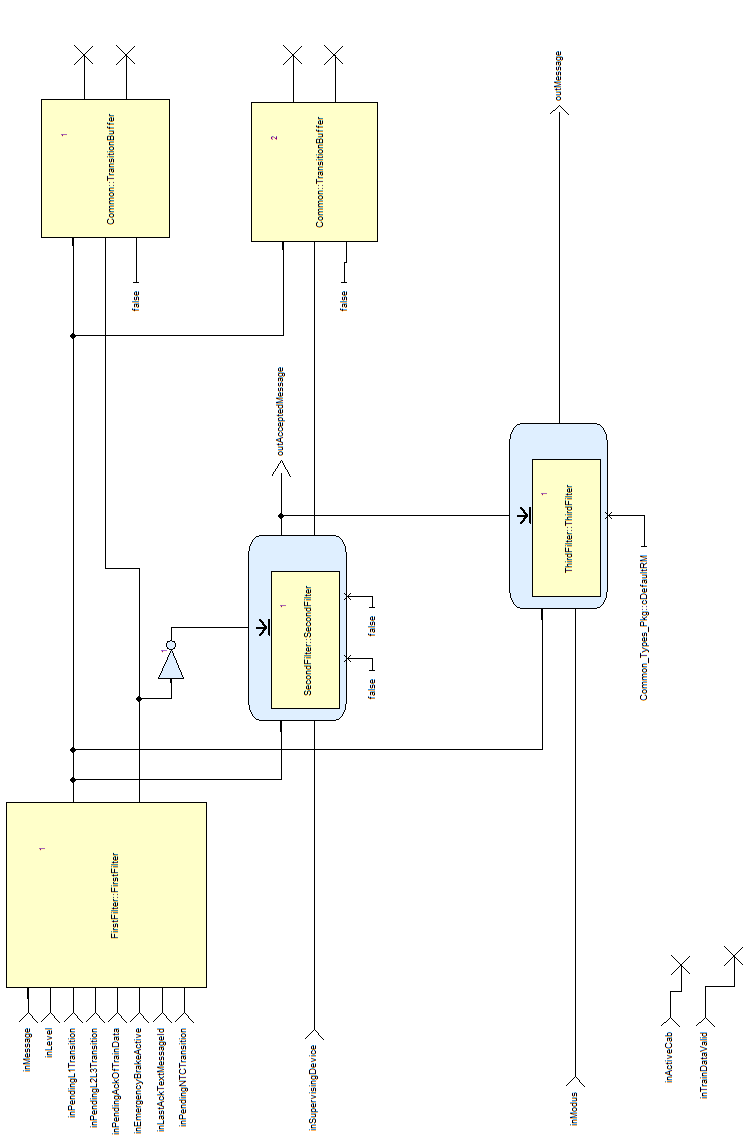
\includegraphics [width=\textwidth]{images/informationfilter-high-level-rot.png}
\caption{High level overview of the InformationFilter components.}
\label{fig:InformationFilterHighLevel}
\end{figure}

\paragraph{Interface}

For an overview of the interface of this internal component we refer to the SCADE model (cf.~link above) respectively the SCADE generated documentation.





\part{Deprecated Design Description}

\chapter{Component Design Template}
%set the master document for easy compilation
%!TEX root = ../D3_5_2.tex

\section{Component Requirements}

\begin{longtable}{p{.25\textwidth}p{.7\textwidth}}
\toprule
Component name			& [Component name] \\
\midrule
Link to SCADE model		& {\footnotesize \url{https://github.com/openETCS/modeling/tree/master/model/Scade/System/ObuFunctions/ManageLocationRelatedInformation/BaliseGroup/Receive_TrackSide_Msg}} \\
\midrule
SCADE designer			& [Name, affiliation] \\
\midrule
Description				& [Brief description of the components functionality] \\
\midrule
Input documents	& 
Subset-026, version, chapter ?.?\newline
Subset-026, version, chapter ?.?\newline
Subset-026, version, chapter ?.?.?\\
\midrule
Safety integrity level		& 4 \\
\midrule
Time constraints		& [If applicable description of time constraints, otherwise n/a] \\
\midrule
API requirements 		& [If applicable description of API requirements, otherwise n/a] \\
\bottomrule
\end{longtable}


\section{Interface}

An overview of the interface of component [component name] is shown in Figure~\ref{f:template_interface}. The inputs and outputs are described in detail in Section~\ref{s:template_inputs} respectively \ref{s:template_outputs}.

\begin{figure}
\center
{[Put SysML diagram of component here]}
\caption{Component SysML diagram}\label{f:template_interface}
\end{figure}


\subsection{Inputs}\label{s:template_inputs}

\subsubsection{[Input 1 name]}

\begin{longtable}{p{.25\textwidth}p{.7\textwidth}}
\toprule
Input name				& [Name of the input] \\
\midrule
Description				& [Brief description of the input] \\
\midrule
Source					& [Name of the source component] \\ 
\midrule
Type					& [Type of the input] \\
\midrule
Valid range of values	& [Complete list of valid values] \\
\midrule
Behaviour when value is at boundary	& [Description of components behaviour when input value is at boundary] \\
\midrule
Behaviour for values out of valid range	& [Description of components behaviour when input value is out of valid range] \\
\bottomrule
\end{longtable}


\subsubsection{[Input 2 name]}

\begin{longtable}{p{.25\textwidth}p{.7\textwidth}}
\toprule
Input name				& [Name of the input] \\
\midrule
Description				& [Brief description of the input] \\
\midrule
Source					& [Name of the source component] \\ 
\midrule
Type					& [Type of the input] \\
\midrule
Valid range of values	& [Complete list of valid values] \\
\midrule
Behaviour when value is at boundary	& [Description of components behaviour when input value is at boundary] \\
\midrule
Behaviour for values out of valid range	& [Description of components behaviour when input value is out of valid range] \\
\bottomrule
\end{longtable}


\subsection{Outputs}\label{s:template_outputs}

\subsubsection{[Output 1 name]}

\begin{longtable}{p{.25\textwidth}p{.7\textwidth}}
\toprule
Output name				& [Name of the output] \\
\midrule
Description				& [Brief description of the output] \\
\midrule
Destination				& [Name of the destination component(s)] \\ 
\midrule
Type					& [Type of the output] \\
\midrule
Valid range of values	& [Complete list of valid values] \\
\midrule
Behaviour when value is at boundary	& [Description of components behaviour when output value is at boundary] \\
\midrule
Behaviour for values out of valid range	& [Description of components behaviour when output value is out of valid range] \\
\bottomrule
\end{longtable}


\subsubsection{[Output 2 name]}

\begin{longtable}{p{.25\textwidth}p{.7\textwidth}}
\toprule
Output name				& [Name of the output] \\
\midrule
Description				& [Brief description of the output] \\
\midrule
Destination				& [Name of the destination component(s)] \\ 
\midrule
Type					& [Type of the output] \\
\midrule
Valid range of values	& [Complete list of valid values] \\
\midrule
Behaviour when value is at boundary	& [Description of components behaviour when output value is at boundary] \\
\midrule
Behaviour for values out of valid range	& [Description of components behaviour when output value is out of valid range] \\
\bottomrule
\end{longtable}


\chapter{F1: Receive information from Trackside}

\chapter{F2: ETCS Kernel}
%-----------------------------------------------------------------------
\subsection{Manage\_TrackSideInformation\_Integration}
%-----------------------------------------------------------------------
%\tbc
%Bernd Hekele

The block ``Manage\_TrackSideInformation\_Integration'' is responsible for receiving Eurobalise-telegrams and Euroradio-messages from the API and perform several consistency checks on the input.

The block collects the telegrams of balises in order to build balise group messages. Euroradio messages are always delivered as a whole message. 

On each message, a consistency check is performed, before the data is validated according to the driving direction of the train. In general, messages not designated for the current driving direction of the train are not forwarded to the further processing.

After applying consistency checks, the data direction is validated.

%Information of the odometer is used to control for the train leaving the expectation window of the balises. % TODO makes not much sense here.

\begin{figure}[H]
 \centering
 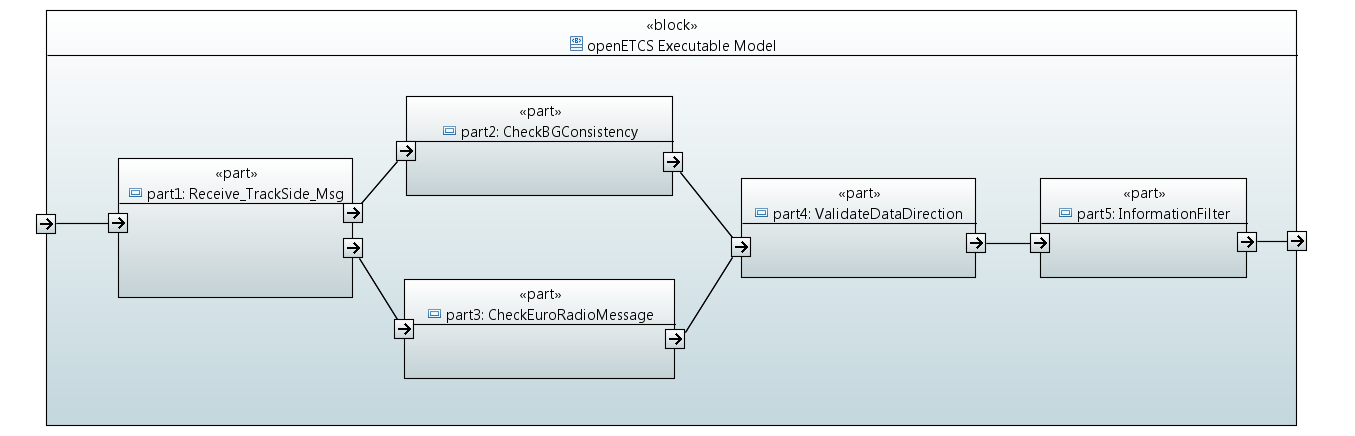
\includegraphics[width=\textwidth]{./images/Input-Messages4.PNG}
 % Input-Messages4.PNG: 0x0 pixel, 0dpi, nanxnan cm, bb=
 \caption{Structure of the Manage\_TrackSideInformation\_Integration module with submodules}
 \label{fig:receiveAndCheckConsistencyArch}
\end{figure}


\subsubsection{Input}
For providing the output, the module needs different input data flows. An overview is provided in table \ref{tbl:ReceiveMessageAndCheckConsistencyInput}

\begin{minipage}{\linewidth}
  \scriptsize
  \begin{tabular}{| c | l | l | l | l |}
    \hline
    \textbf{Index} & \textbf{Input name} & \textbf{Input type} & \textbf{Source}\\ \hline
    0 & \texttt{fullChecks} & \texttt{bool} & Configuration \\
    1 & \texttt{API\_trackSide\_Message} & \texttt{API\_Msg\_Pkg::API\_TrackSideInput\_T} & API\\
    2 & \texttt{ActualOdometry} & \texttt{Obu\_BasicTypes\_Pkg::odometry\_T} & Odometer\\
    3 & \texttt{reset} & \texttt{bool} & Environment\\
    4 & \texttt{trainPosition} & \texttt{TrainPosition\_Types\_Pck::trainPosition\_T} & Calculate Train Position\\
    5 & \texttt{modeAndLevel} & \texttt{BG\_Types\_Pkg::ModeAndLevelStatus\_T} & Mode and Level\\
    6 & \texttt{tNvContact} & \texttt{Obu\_BasicTypes\_Pkg::T\_internal\_Type} & Database\\
    7 & \texttt{lastRelevantEventTimestamp} & \texttt{Obu\_BasicTypes\_Pkg::T\_internal\_Type} & Database\\
    8 & \texttt{connectionStatus} & \texttt{Radio\_Types\_Pkg::sessionStatus\_Type} & Manage Radio Communication\\
    9 & \texttt{inSupervisingRbcId} & \texttt{int} & Database\\
    10 & \texttt{inAnnouncedBGs} & \texttt{TrainPosition\_Types\_Pck::positionedBGs\_T} & Calculate Train Position\\
    11 & \texttt{q\_nvlocacc} & \texttt{Q\_NVLOCACC} & Database\\
    \hline
  \end{tabular} 
  \captionof{table}{Overview over input}
  \label{tbl:ReceiveMessageAndCheckConsistencyInput}
\end{minipage}

\paragraph{Input 0: \texttt{fullChecks\\}}
The boolean indicates, if all checks on the message should be performed. The possible values are given in table \ref{tbl:fullChecks}.

\begin{minipage}{\linewidth}
 \begin{tabular}{| l | p{9cm} |}
    \hline
    \textbf{Value} & \textbf{Interpretation}\\ \hline
    true & All checks are performed.\\
    false & The module \texttt{Information Filter} is deactivated.\\
    \hline
  \end{tabular} 
  \captionof{table}{Possible values for the input \texttt{fullChecks}}
  \label{tbl:fullChecks}
\end{minipage}

\paragraph{Input 1: \texttt{API\_trackSide\_Message}}

The \texttt{API\_trackSide\_Message} is the message received from the API. The API performs preprocessing of RTM and BTM messages and deliveres a maximum of a single message per cycle to the SCADE model.

\paragraph{Input 2: \texttt{ActualOdometry}}
The input \texttt{ActualOdometry} is provided by the external odometry module of the train. It contains location information with inaccuracies.

\paragraph{Input 3: \texttt{reset}\\}
To delete all data stored in the module (e.g. collected balise-telegrams, which do not yet form a complete message), a reset input can be used. If the input is set to \texttt{true}, all data kept in the module is deleted and no input is accepted.

\begin{minipage}{\linewidth}
   \begin{tabular}{| l | p{9cm} |}
    \hline
    \textbf{Value} & \textbf{Interpretation}\\ \hline
    true & All data kept in the module is deleted and no input is accepted.\\
    false & No action. Data at input is accepted.\\
    \hline
  \end{tabular} 
  \captionof{table}{Possible values for the input \texttt{reset}}
  \label{tbl:reset}
\end{minipage}


\paragraph{Input 4: \texttt{trainPosition}}
The input \texttt{trainPosition} is generated by the ``Calculate Train Position'' module and contains the current position of the train.

\paragraph{Input 5: \texttt{modeAndLevel}}
The input is generated by the ``Mode and level management'' module. It provides the current level and mode of the EVC.

\paragraph{Input 6: \texttt{tNvContact}}

For monitoring the safe radio connection, the national value \texttt{T\_NVCONTACT} is needed as an input.

\paragraph{Input 7: \texttt{lastRelevantEventTimestamp}}

For monitoring the safe radio connection, it's necessary, that the time between two packets is less than the value of \texttt{T\_NVCONTACT}.

In situations like level-changes or announced radioholes, not the timestamp of the last message is relevant for comparison, but the timestamp of the last relevant event. This can be e.g. the timestamp of the level change or the timestamp of the timestamp of the moment, when the train was passing the end of the radiohole. 

For performing this check, the timestamp of the last relevant event is provided to the model as an \texttt{T\_internal\_Type}-type.

\paragraph{Input 8: \texttt{connectionStatus}\\}
The input \texttt{connectionStatus} will give information about the radio connection. This input is delivered by the session management module, not from the API. The information is needed to perform the timing check, which is depending on the connection state.

\begin{minipage}{\linewidth}
  \begin{tabular}{| l | p{9cm} |}
    \hline
    \textbf{Value} & \textbf{Interpretation}\\ \hline
    DISCONNECTED & The OBU is currently not connected to a RBC.\\
    CONNECTING & The OBU is currently connecting to the RBC. Received messages belong to the process of establishing a connection.\\
    CONNECTION\_ESTABLISHED &  The connection to RBC is established.\\
    \hline
  \end{tabular} 
  \captionof{table}{Possible values for the input \texttt{connectionStatus}}
  \label{tbl:connectionStatus}
\end{minipage}

\paragraph{Input 9: \texttt{inSupervisingRbcId}}
For the submodule ``Information Filter'', the information is needed, which radio messages are sent by the supervising RBC. To recognize these messages, the identifier of the supervising RBC is needed.

\paragraph{Input 10: \texttt{inAnnouncedBGs}}
This input provides information about balise groups which will be passed by the train soon. This information is generated by ``Calculate Train Position'' based on the linking information received from trackside.

\paragraph{Input 11: \texttt{q\_nvlocacc}}
The national value determines the location accuracy and is delivered by the database.



\subsubsection{Output}
The output of the module provides the received and processed Euroradio and Eurobalise messages. The module combines messages both from Eurobalises and from Euroradio to one common dataflow.

An overview over the output dataflows is provided in table \ref{tbl:ReceiveMessageAndCheckConsistencyOutput}.

\begin{minipage}{\linewidth}
 \footnotesize
  \begin{tabular}{| c | l | l | l |}
    \hline
    \textbf{Index} & \textbf{Output name} & \textbf{Output type}\\ \hline
    0 & \texttt{outputMessage} & \texttt{Common\_Types\_Pkg::ReceivedMessage\_T}\\
    1 & \texttt{ApplyServiceBrake} & \texttt{bool}\\
    2 & \texttt{BadBAliseMessageToDMI} & \texttt{bool}\\
    3 & \texttt{errorLinkedBG} & \texttt{bool}\\
    4 & \texttt{errorUnlinkedBG} & \texttt{bool}\\
    5 & \texttt{passedBG} & \texttt{BG\_Types\_Pkg::passedBG\_T} \\
    6 & \texttt{outPositionParams} & \texttt{Common\_Types\_Pkg::PositionReportParameter\_T} \\
    7 & \texttt{outRadioManagement} & \texttt{Common\_Types\_Pkg::radioManagementMessage\_T} \\
    8 & \texttt{radioSequenceError} & \texttt{bool} \\
    9 & \texttt{radioMessageConsistencyError} & \texttt{bool} \\
    \hline
  \end{tabular} 
  \captionof{table}{Dataflow at output}
  \label{tbl:ReceiveMessageAndCheckConsistencyOutput}
\end{minipage}

\subparagraph{Output 0: \texttt{outputMessage}\\}
The element \texttt{outputMessage} consists of the type \texttt{ReceivedMessage\_T} combines both balise and radio messages to one common datatype. This datatype contains all variables and packets, which are possible for the given scenario.

\begin{minipage}{\linewidth}
  \scriptsize
  \begin{tabular}{| l | l | p{5.5cm} |}
  \hline
  \textbf{Name} & \textbf{Datatype} & \textbf{Description}\\ \hline
  \texttt{valid} & \texttt{bool} & true, if no consistency errors were detected.\\
  \texttt{source} & \texttt{Common\_Types\_Pkg::MsgSource\_T} & Defines, if this is a Euroradio or Eurobalise message.\\
  \texttt{packetMetadata} & \texttt{Common\_Types\_Pkg::Metadata\_T} & contains the metadata of the packets\\
  \texttt{radioMetadata} & \texttt{Common\_Types\_Pkg::RadioMetadata\_T} & contains the metadata of the radio specific header variables\\
  \texttt{BG\_Common\_Header} & \texttt{BG\_Types\_Pkg::BG\_Header\_T} & Header of Eurobalise message\\
  \texttt{Radio\_Common\_Header} & \texttt{Radio\_Types\_Pkg::Radio\_TrackTrain\_Header\_T} & Header of Euroradio message\\
  \texttt{packets} & Common\_Types\_Pkg::Packets\_T & Structure of packets in messages\\
  \hline
\end{tabular}
  \captionof{table}{Structure of \texttt{ReceivedMessage\_T}}
  \label{tbl:receivedMessage_structure}
\end{minipage}


The Eurobalise-common-header \texttt{BG\_Header\_T} consists of the fields visible in the SCADE-declaration. The structure corresponds to the structure defined in the SRS chapter 8.4.2.1. Some fields were removed since they are not needed anymore for further processing after building messages from separate telegrams.

The Euroradio-common-header \texttt{Radio\_TrackTrain\_Header\_T} consists of the fields visible in the SCADE declaration. The structure corresponds to the structure defined in the SRS chapter 8.4.4.6.1. The structure contains all variables required by possible \texttt{NID\_MESSAGE} values for the given scenario. Which values are valid is defined in the field \texttt{radioMetadata}.

%\textbf{TODO:} Different definition of Radio-header than in SCADE!

%\textbf{TODO:} Note on packet type definitions and implementation details (which values were not used).

%\textbf{Note:} Packet 44 not used (applications outside the ERTMS/ETCS system are not supported by this implementation).

%\textbf{TODO:} Define packets 136, 12 in SCADE.

\subparagraph{Output 1: \texttt{ApplyServiceBreak}}
The flag indicates the balise group the train just passed could not be processed correctly. The check results in the request for a service break.

\subparagraph{Output 2: \texttt{BadBaliseMessageToDMI}}
Information to be passed to the DMI to indicate the reception of a ``bad balise'' to the driver.

\subparagraph{Output 3: \texttt{errorLinkedBG}\\}

\begin{minipage}{\linewidth}
  \begin{tabular}{| l | p{9cm} |}
    \hline
    \textbf{Value} & \textbf{Interpretation}\\ \hline
    true & A error in a linked balise group was detected.\\
    false & No error in a linked balise group was detected.\\
    \hline
  \end{tabular} 
  \captionof{table}{Possible values for the input \texttt{errorLinkedBG}}
  \label{tbl:errorLinkedBG}
\end{minipage}

\subparagraph{Output 4: \texttt{errorUnlinkedBG}\\}
\begin{minipage}{\linewidth}
  \begin{tabular}{| l | p{9cm} |}
    \hline
    \textbf{Value} & \textbf{Interpretation}\\ \hline
    true & A error in an unlinked balise group was detected.\\
    false & No error in an unlinked balise group was detected.\\
    \hline
  \end{tabular} 
  \captionof{table}{Possible values for the input \texttt{errorUnlinkedBG}}
  \label{tbl:errorUnlinkedBG}
\end{minipage}

\subparagraph{Output 5: \texttt{passedBG}}
The output \texttt{passedBG} provides the received balise group message in a special format needed by the module ``Calculate train position''.

\subparagraph{Output 6: \texttt{outPositionParams}}
The output \texttt{outPositionParams} provides the parameters for the position report in a special format needed by the module ``Provide Position Report''.

\subparagraph{Output 7: \texttt{outRadioManagement}}
The output \texttt{outRadioManagement} provides the messages for radio session management in a special format needed by the module ``Management of Radio Communication''.

\subparagraph{Output 8: \texttt{radioSequenceError\\}}

\begin{minipage}{\linewidth}
  \begin{tabular}{| l | p{9cm} |}
    \hline
    \textbf{Value} & \textbf{Interpretation}\\ \hline
    true & A sequence error or a timeout has been detected in the radio message.\\
    false & No error in the radio message sequence was detected.\\
    \hline
  \end{tabular} 
  \captionof{table}{Possible values for the input \texttt{radioSequenceError}}
  \label{tbl:radioSequenceError}
\end{minipage}

\subparagraph{Output 9: \texttt{radioMessageConsistencyError\\}}

\begin{minipage}{\linewidth}
  \begin{tabular}{| l | p{9cm} |}
    \hline
    \textbf{Value} & \textbf{Interpretation}\\ \hline
    true & A consistency error has been detected in the radio message.\\
    false & No consistency error in the radio message was detected.\\
    \hline
  \end{tabular} 
  \captionof{table}{Possible values for the input \texttt{radioMessageConsistencyError}}
  \label{tbl:radioMessageConsistencyError}
\end{minipage} 

~\\

\subsubsection{Receive\_TrackSide\_Msg in Manage\_TrackSideInformation\_Integration}

\paragraph{Reference to the SRS (or other requirements)}
\begin{itemize}
  \item \cite[Chapt.~7 and 8]{subset-026}: Definition of the Balise Telegram
  \item \cite[Chapt.~4.2.2, 4.2.4, 4.2.9]{subset-036}: Interface to the BTM
  \item \cite[Chapt.~3.4.1 - 3.4.3, 3.16.2]{subset-026}: Handling of Balise Telegrams
  \item \cite[Chapt.~3.16.2]{subset-026}: Check of the balise group
  \item \cite[Chapt.~3.4.2]{subset-026}: Determining the orientation
  \item \cite[Chapt.~4.5.2]{subset-026}: Active Functions Table
  \item \cite[Chapt.~8.4.4]{subset-026}: Rules for Euroradio messages

\end{itemize}
\paragraph{Short description of the functionality}
This function defines the interface of the OBU model to the openETCS generic API for Eurobalise  and Euroradio messages. On the interface, either a valid telegram/message is provided or a telegram/message is indicated which could not be received correct when passing the balise or receiving the radio message. The function passes a balise telegram without major changes of the information to the next entity for collecting the balise group information. This entity collects telegrams received via the interface into Balise Group Information. In case of a radio message, the message is converted to an internal format for further processing and passed without changing the information contained.

\paragraph{Interface}
\paragraph{Functional Design Description}
\textbf{Design Constraints and Choices}
\begin{enumerate}
\item The decoding of balises is done at the API. Also, packets received via the interface are already transformed into a usable shape.
\item Only packets used inside the current model are passed via the interface.\\
\item Treatment of Packet 5: Linking Information.\\
Linking Information is added to the linking array starting from index 0 without gaps. Used elements are marked as valid. Elements are sorted according to the order given by the telegram sequence.
\item Telegrams received as invalid are passed to the ``Check-Function'' to process errors in communication with the track side according to the requirements and in a single place.
Telegrams are added to the telegram array starting from index 0 without gaps. Used elements are marked as valid. Elements are stored according to the order given by the telegram sequence.
\item This function does not process information from the packets. The information is passed to the check without further processing of the values. 
\end{enumerate}
\paragraph{Reference to the Scade Model}
The SCADE model can be found on github under the following path:

\tiny\url{https://github.com/openETCS/modeling/tree/master/model/Scade/System/ObuFunctions/ManageLocationRelatedInformation/BaliseGroup/Receive_TrackSide_Msg}
\normalsize
\subsubsection{CheckBGConsistency in Manage\_TrackSideInformation\_Integration}%Mainfunction receive track data. Name should be be defined and substituded by the designer of the function. 
\paragraph{Reference to the SRS or other Requirements (or other requirements)}
\begin{itemize}
  \item \cite[Chapt.~7 and 8]{subset-026}: Definition of the Balise Telegram
  \item \cite[Chapt.~3.4.1 - 3.4.3, 3.16.2]{subset-026}: Handling of Balise Telegrams
  \item \cite[Chapt.~3.16.2]{subset-026}: Check of the balise group
  \item \cite[Chapt.~4.5.2]{subset-026}: Active Functions Table
\end{itemize}
\paragraph{Short description of the functionality}
This function has the task  to verify the completeness and correctness of the received messages from balise groups.\\
A message consists of at least a telegram and a maximum of 8 telegrams.\\

\begin{itemize}
\item A message is still complete and correct, if a telegram is missing (or not decoded or incomplete decoded ), and this telegram is duplicated within the balise group and the duplicating one is correctly read.
\item By more than one telegram, the order of the telegrams must be either ascending (nominal) or descending(reverse).\\
\item A message is correct, if  all message counters (M MCUNT) do not equal 254 (that means: The telegram never fits any message of the group).\\ A message counter can be equal 255 (that means: The telegram fits with all telegrams of the same balise group) and all other values must be the same.\\
\end{itemize}

\paragraph{Interface}
An input of the operator is a list of recived telegrams. \\
After consistency check of the telegrams' list, the function generates the balise-group-message.\\
This function is active in certain modes and the output and reactions are dependent on if the linking information is used.\\

\paragraph{Functional Design Description}
The orientation of the BG will also be calculated in this block.\\
The check, if the message has been received in due time and the right at the right expected location, will be performed in "Calculate Train Position".\\
The checks on the validity of the data in the packets and the validity with respect to the direction of motion will be performed in other modules, e.g. "Validate Data Direction" .

\paragraph{Reference to the Scade Model}
The SCADE model can be found on github under the following path:

\tiny\url{https://github.com/openETCS/modeling/tree/master/model/Scade/System/ObuFunctions/ManageLocationRelatedInformation/BaliseGroup/CheckBGConsistency}
\normalsize

\subsubsection{CheckEuroradioMessage in Manage\_TrackSideInformation\_Integration}%Mainfunction receive track data. Name should be be defined and substituded by the designer of the function. 
\paragraph{Reference to the SRS or other Requirements (or other requirements)}
\begin{itemize}
 \item \cite[Chapt.~8.4.4]{subset-026}: Rules for Euroradio messages
 \item \cite[Chapt.~3.16]{subset-026}: Data consistency
\end{itemize}
\paragraph{Short description of the functionality}

The operator ``CheckEuroradioMessage'' performs several checks on the received radio message. These checks include checking of the message sequence, completeness of messages. Invalid messages are marked as invalid in the message header.

\paragraph{Interface}
The operator expects a radio message, information about the timestamp of the last relevant event, the national value for timeout (\texttt{T\_NVCONTACT}) and the status of the radio connection as input. The operator provides as output the radio message marked as valid or invalid in the message header and updated metadata in the message. Errors are indicated through boolean outputs.

\paragraph{Functional Design Description}

The operator performs the following checks:
\begin{itemize}
 \item Content checks
 \begin{itemize}
    %\item The computed length of the message must be equal to the value in \texttt{L\_MESSAGE}. (SRS 8.4.4.2.1)
    \item The whole message must be complete and contains all necessary fields. \cite[3.16.1.1]{subset-026}
    \item The message must respect the ETCS language. \cite[3.16.1.1]{subset-026} The operator checks, if all necessary variables and packets for the corresponding message are part of the message and if no packets and variables are included in the message, which are not allowed.
    %\item The variables of the message do not contain invalid values. \cite[3.16.1.1]{subset-026} % already done by API?
    %\item Check if the specified priority of message is equal to the priority with which the message was received. \cite[3.16.3.1.3.1]{subset-026}
  \end{itemize}
  \item Timing checks
  \begin{itemize}
    \item Check if the timestamp of a message is greater than the timestamp of the message received before. \cite[3.16.3.3.3]{subset-026}
    \item If a message contains the timestamp ``Unknown'', check if this message is part of the initiation of the communication session. \cite[3.16.3.3.4]{subset-026}
    \item Perform the check with the current message $n$:  $T\_TRAIN_{n} <= T\_TRAIN_{n-1} + T\_NVCONTACT$ \cite[3.16.1.1]{subset-026}. This ensures, that the message was received in due time.
  \end{itemize}
\end{itemize}

For inconsistent messages, the following actions are performed by the operator:

\begin{itemize}
  \item If a message is not consistent, it shall be rejected. \cite[3.16.3.1.1.1]{subset-026} For this purpose, the message is marked as invalid, so it can be rejected by the operators using the output of the CheckEuroradioMessage-operator.
  \item The RBC shall be informed, when a message was rejected. \cite[3.16.3.1.1.2]{subset-026} Therefore the necessary information for creating an error report is provided as boolean flags. 
  %\item If the RBC requested an ACK for a received message, message will be marked for the module to send a report to the RBC. (SRS 3.16.3.5)
  \item This operator will not trigger the reaction for an interrupted radio connection to the RBC. The reaction sepcified by \texttt{M\_NVCONTACT} will be triggered by the RBC session management module.
\end{itemize}

The check by the Euroradio-protocol \cite[3.16.3.1.1]{subset-026} will not be performed by the operator, but on a lower level (RTM or openETCS-API).

The operator is not responsible for checking the integrity of the message in the bitstream format. The bitwalker, which is converting the bitstream into the internally used datatypes, is performing the checks, which are only possible on the raw data. This includes a CRC check on the whole message and a value range check for each variable. If a consistency error is detected by the bitwalker, it is signalled to the model. If the bitwalker marks a packet as valid, all variables are expected to contain a valid value. The bitwalker is not part of the ETCS kernel.

Safe connection supervision is not in the scope of this operator. This functionality will be implemented by the ``Management of Radio communication'' module.

\paragraph{Reference to the Scade Model}
The SCADE model can be found on github under the following path:

\tiny\url{https://github.com/openETCS/modeling/tree/master/model/Scade/System/ObuFunctions/ManageLocationRelatedInformation/BaliseGroup/CheckEuroRadioMessage}
\normalsize

\subsubsection{ValidateDataDirection in Manage\_TrackSideInformation\_Integration}

\paragraph{Reference to the SRS or other Requirements (or other requirements)}
\begin{itemize}
 \item The functionality is mainly described in \cite[Chapter~3.6.3]{subset-026}.
\end{itemize}
\paragraph{Short description of the functionality}
The operator will filter an input message in order to mark all elements as invalid, which are not designated for the current driving direction of the train.

\paragraph{Interface}
The operator expects a message and information about the LRBG, passed balises and the current train position. As output, the message with packets valid for the current direction of driving is provided.
\paragraph{Functional Design Description}
\begin{itemize}
 \item The operator contains two processing paths for different message types. Radio messages and balise group messages are handeled in a different way. For validating the data direction of a radio message, the check is performed using the balise group referenced in the radio message header as relevant balise group. For balise group message, the LRBG is used.
 \item The metadata of packets, which are recognized as not valid for the current driving direction, is invalidated.
\end{itemize}

\paragraph{Reference to the Scade Model}
The SCADE model can be found on github under the following path:

\tiny\url{https://github.com/openETCS/modeling/tree/master/model/Scade/System/ObuFunctions/ManageLocationRelatedInformation/BaliseGroup/ValidateDataDirection}
\normalsize

\subsubsection{InformationFilter}

\paragraph{Reference to the SRS and other requirements}
\begin{itemize}
 \item The functionality of the InformationFilter is described in \cite[Chapter~4.8]{subset-026}.
\end{itemize}

\paragraph{Short description of the functionality}
The function InformationFilter filters incoming information received
from Eurobalise, Euroradio, and Euroloop. The information is received
via messages and filtering is done depending on the criteria described
in \cite[Chapter~4.8]{subset-026}. Messages are only allowed to pass
the filter if specified critera are met like for example the correct
mode of the train (e.g. Full Supervision, Shunting, etc.) or the ETCS
level. Some messages have to be stored in a TransitionBuffer to be
later reevaluated by the filter again.

\paragraph{Interface}
The interface of the information filter contains mainly the incoming
message and inputs to check for the conditions described in the
SRS. The complete interface is shown in table \ref{tbl:InformationFilterInterface}.

\begin{minipage}{\linewidth}
  \scriptsize
  \begin{tabular}{| l | l | l |}
    \hline
    \textbf{Name}                    & \textbf{Direction} & \textbf{Description}                                        \\ 
    \hline
    \texttt{inMessage}               & \texttt{IN}        & Received message that is valid for the train direction      \\
    \texttt{inLevel}                 & \texttt{IN}        & The current ETCS Level                                      \\
    \texttt{inMode}                  & \texttt{IN}        & The current train mode                                      \\
    \texttt{inSupervisingDevice}     & \texttt{IN}        & The device id which communicates with the current supervising
  RBC                                                                                                                   \\
    \texttt{inPendingL1Transition}   & \texttt{IN}        & Information if an ETCS Level 1 transition is pending        \\
    \texttt{inPendingL1L2Transition} & \texttt{IN}        & Information if an ETCS Level 2/3 transition is pending      \\
    \texttt{inPendingNTCTransition}  & \texttt{IN}        & Information if a NTC transition is pending                  \\
    \texttt{inPendingAckOfTrainData} & \texttt{IN}        & Information if the acknowledgement of train data is pending \\
    \texttt{inEmergencyBrakeActive}  & \texttt{IN}        & Information if the emergency brake is active                \\
    \texttt{inLastAckTextMessageId}  & \texttt{IN}        & The id of the last acknowledged message ID                  \\
    \texttt{inActiveCab}             & \texttt{IN}        & Information if the cab is active                            \\
    \texttt{inTrainDataValid}        & \texttt{IN}        & Information if the train data is valid                      \\
    \texttt{outMessage}              & \texttt{OUT}       & The filtered input message                                  \\
    \hline
  \end{tabular}
  \captionof{table}{Overview of the InformationFilter interface}
  \label{tbl:InformationFilterInterface}
\end{minipage}

\paragraph{Functional Design Description}

\begin{figure}[hbtp]
\centering
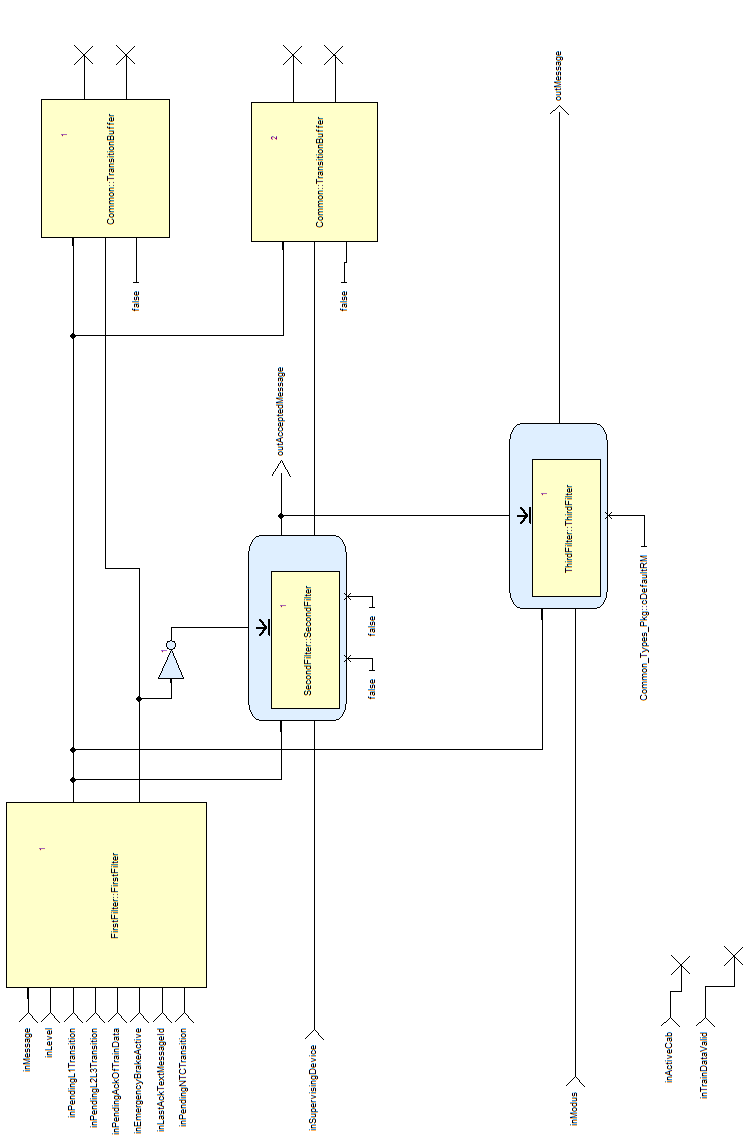
\includegraphics [scale=0.8]{images/informationfilter-high-level-rot.png}
\caption{High level overview of the InformationFilter components.}
\label{fig:InformationFilterHighLevel}
\end{figure}

The filter receives track information (balise and radio) and filter
them depending of the mode, level and further information. Only
messages that pass the filter are valid and should be considered by
other ETCS subsystems. The figure \ref{fig:InformationFilterHighLevel}
show the high\-level decomposition of the functionality. The filter
functionality can be decomposed into a FirstFilter, SecondFilter,
ThirdFilter an TransitionBuffer.

\paragraph{FirstFilter} This filter performs filtering of messages
based on the current ETCS level. The decisions taken process is
described via a big decision table which contains rows for every
packet and columns for every ETCS level. This table encodes also if
certain additional information is necessary to filter a message like
pending ETCS Level transitions. Based on this filter packets of an
incoming message is either rejected, accepted or the whole message is
put in the TransitionBuffer. Messages are put in the TransitionBuffer
if there is an announced level transition and the received message is
only valid for the upcoming level.

\paragraph{SecondFilter} The SecondFilter mainly considers messages
that are received via Euroradio. Certain messages are directly
rejected while other may be stored in the TransitionBuffer. The buffer
is used to store messages that are received from non supervising RBCs,
but will be reevaluated after a RBC transition.

\paragraph{ThirdFilter} The last filter is functionally very similiar
the the FirstFilter, however it filters depending on the mode. It also
contains a decision table with rows for every packet but the columns
are modes.

\paragraph{TransitionBuffer} The InformationFilter uses two
TransitionBuffers. One is used to store up to three messages for the
ETCS level transition and the other buffer is used for RBC
transitions. The buffer is designed as a ring buffer and message are
read in FIFO order.

A detailed list of packages and their handling depending of ETCS level
or mode can be seen in table \ref{fig:PackagesListLevel} and
\ref{fig:PackagesListMode}.

\begin{figure}[hbtp]
\centering
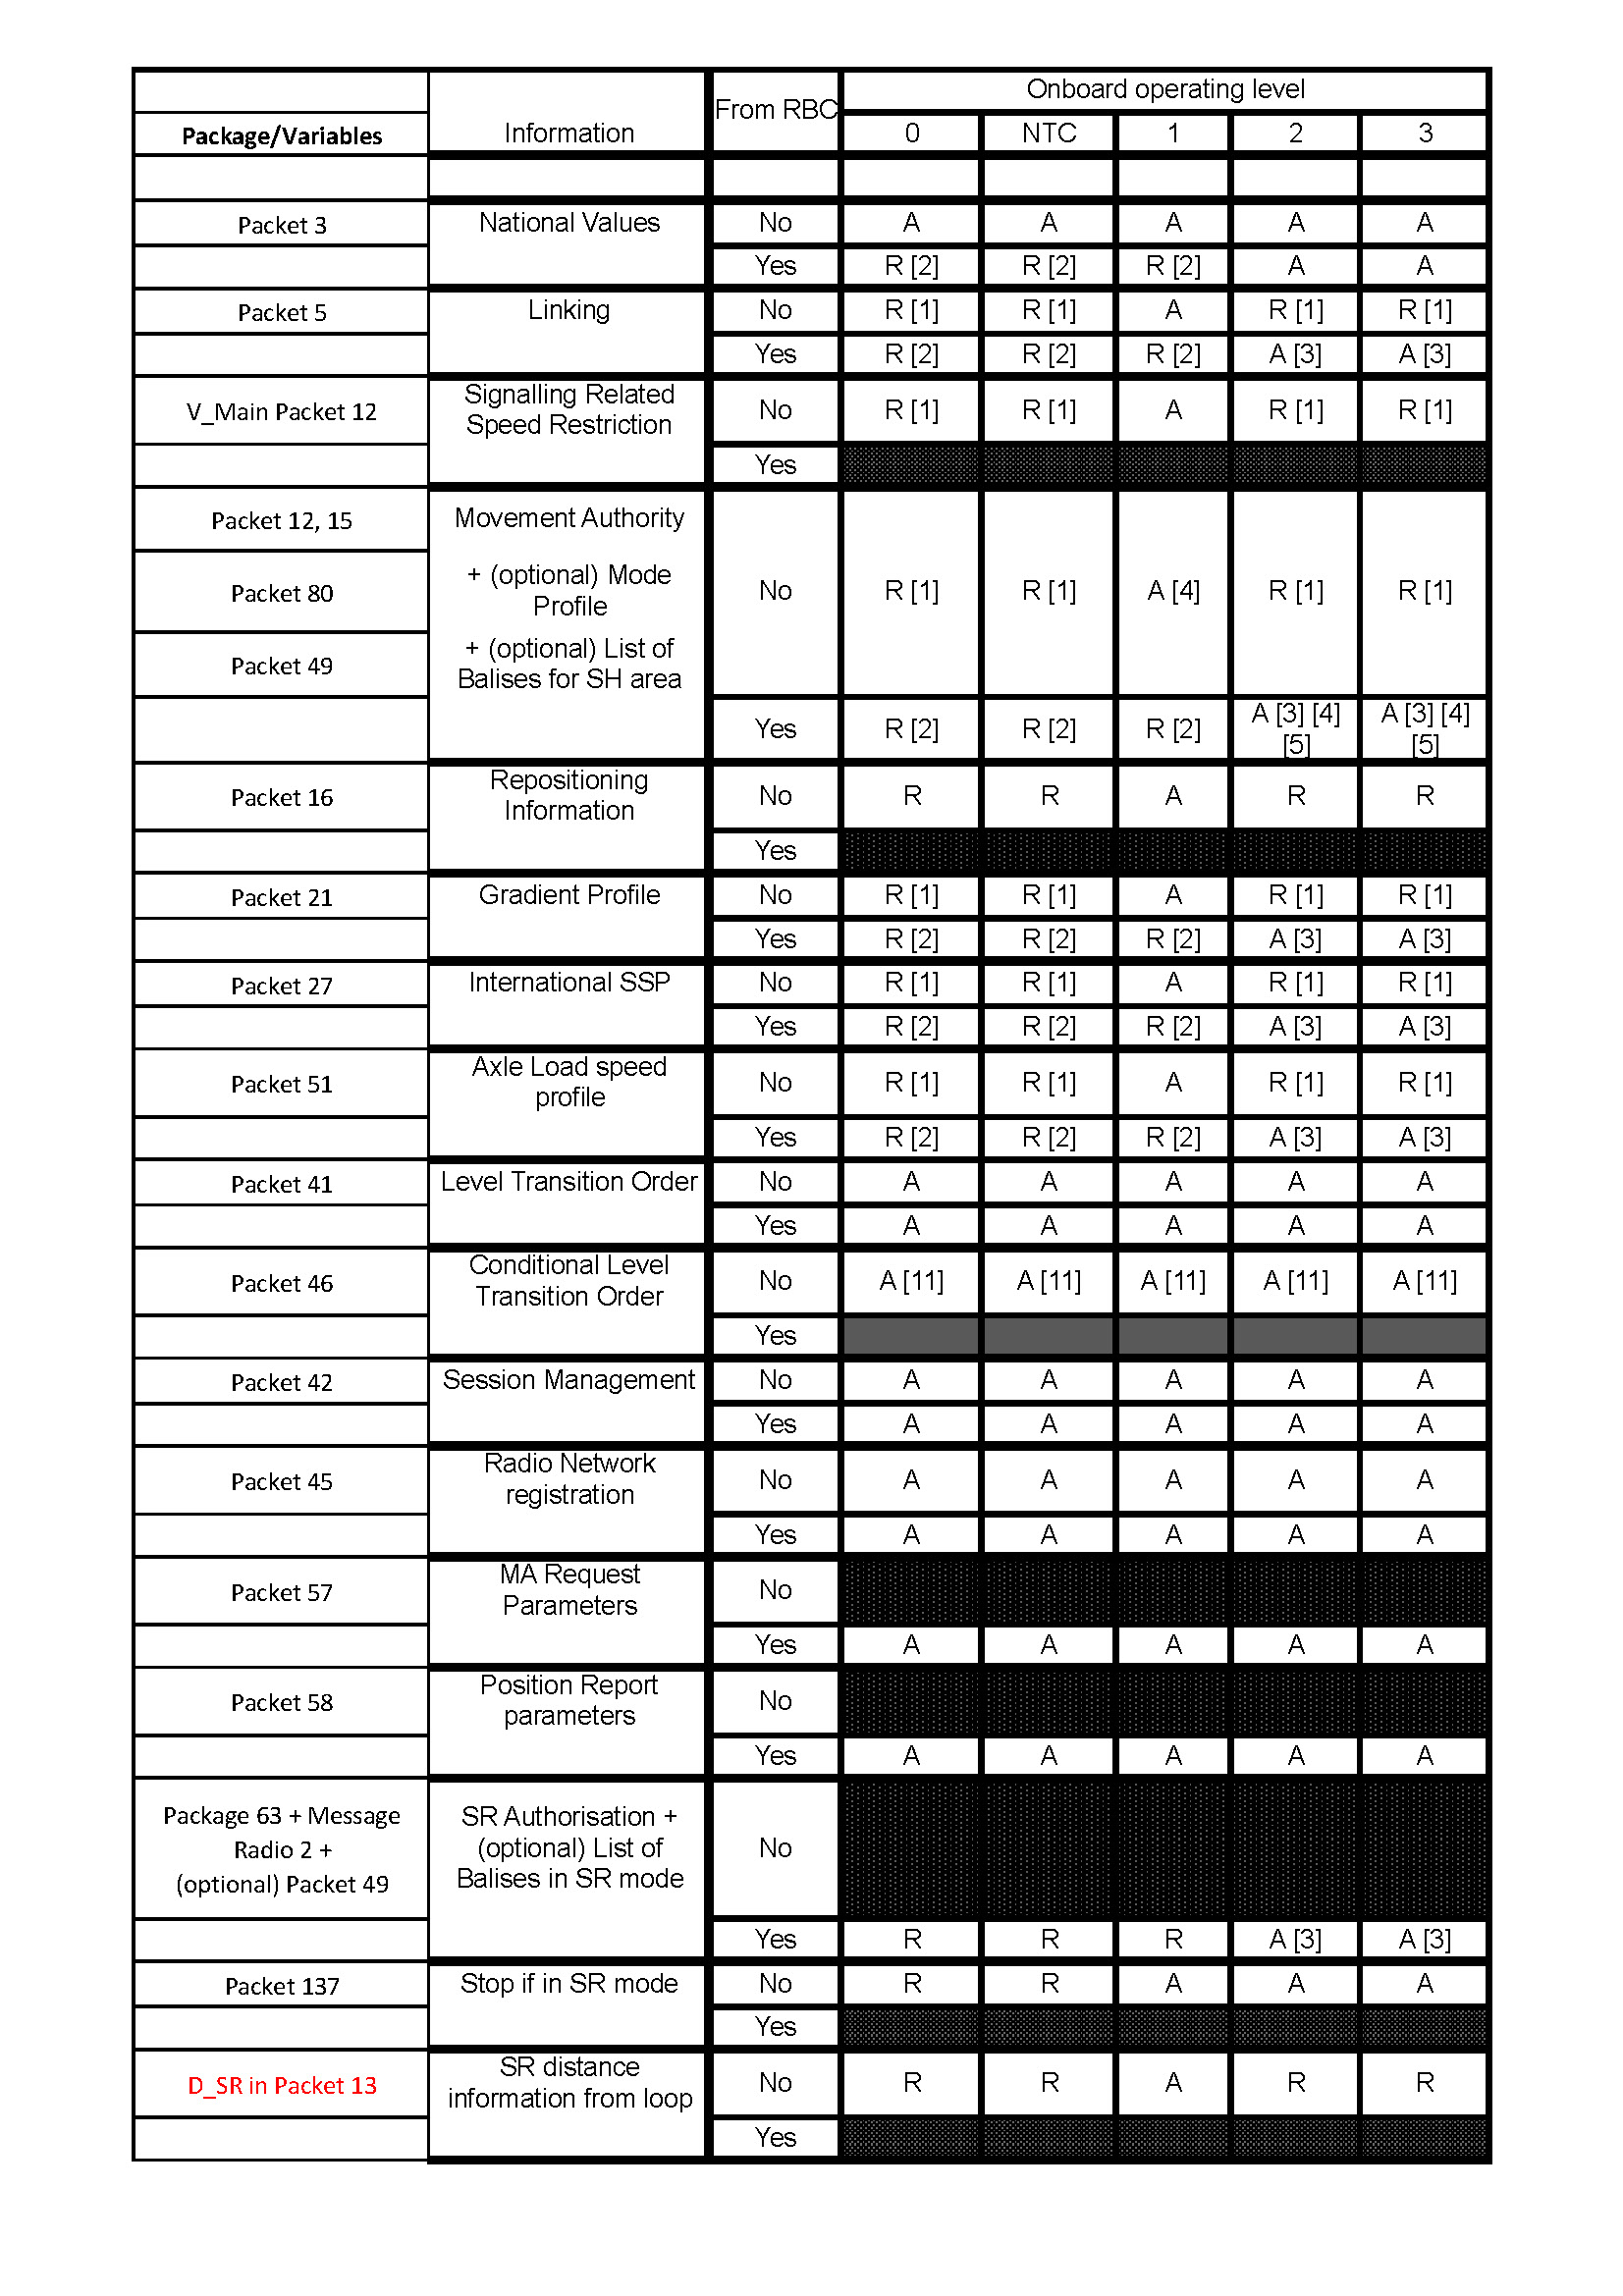
\includegraphics [scale=0.6]{images/LevelFilter1}
\end{figure}
\begin{figure}[hbtp]
\centering
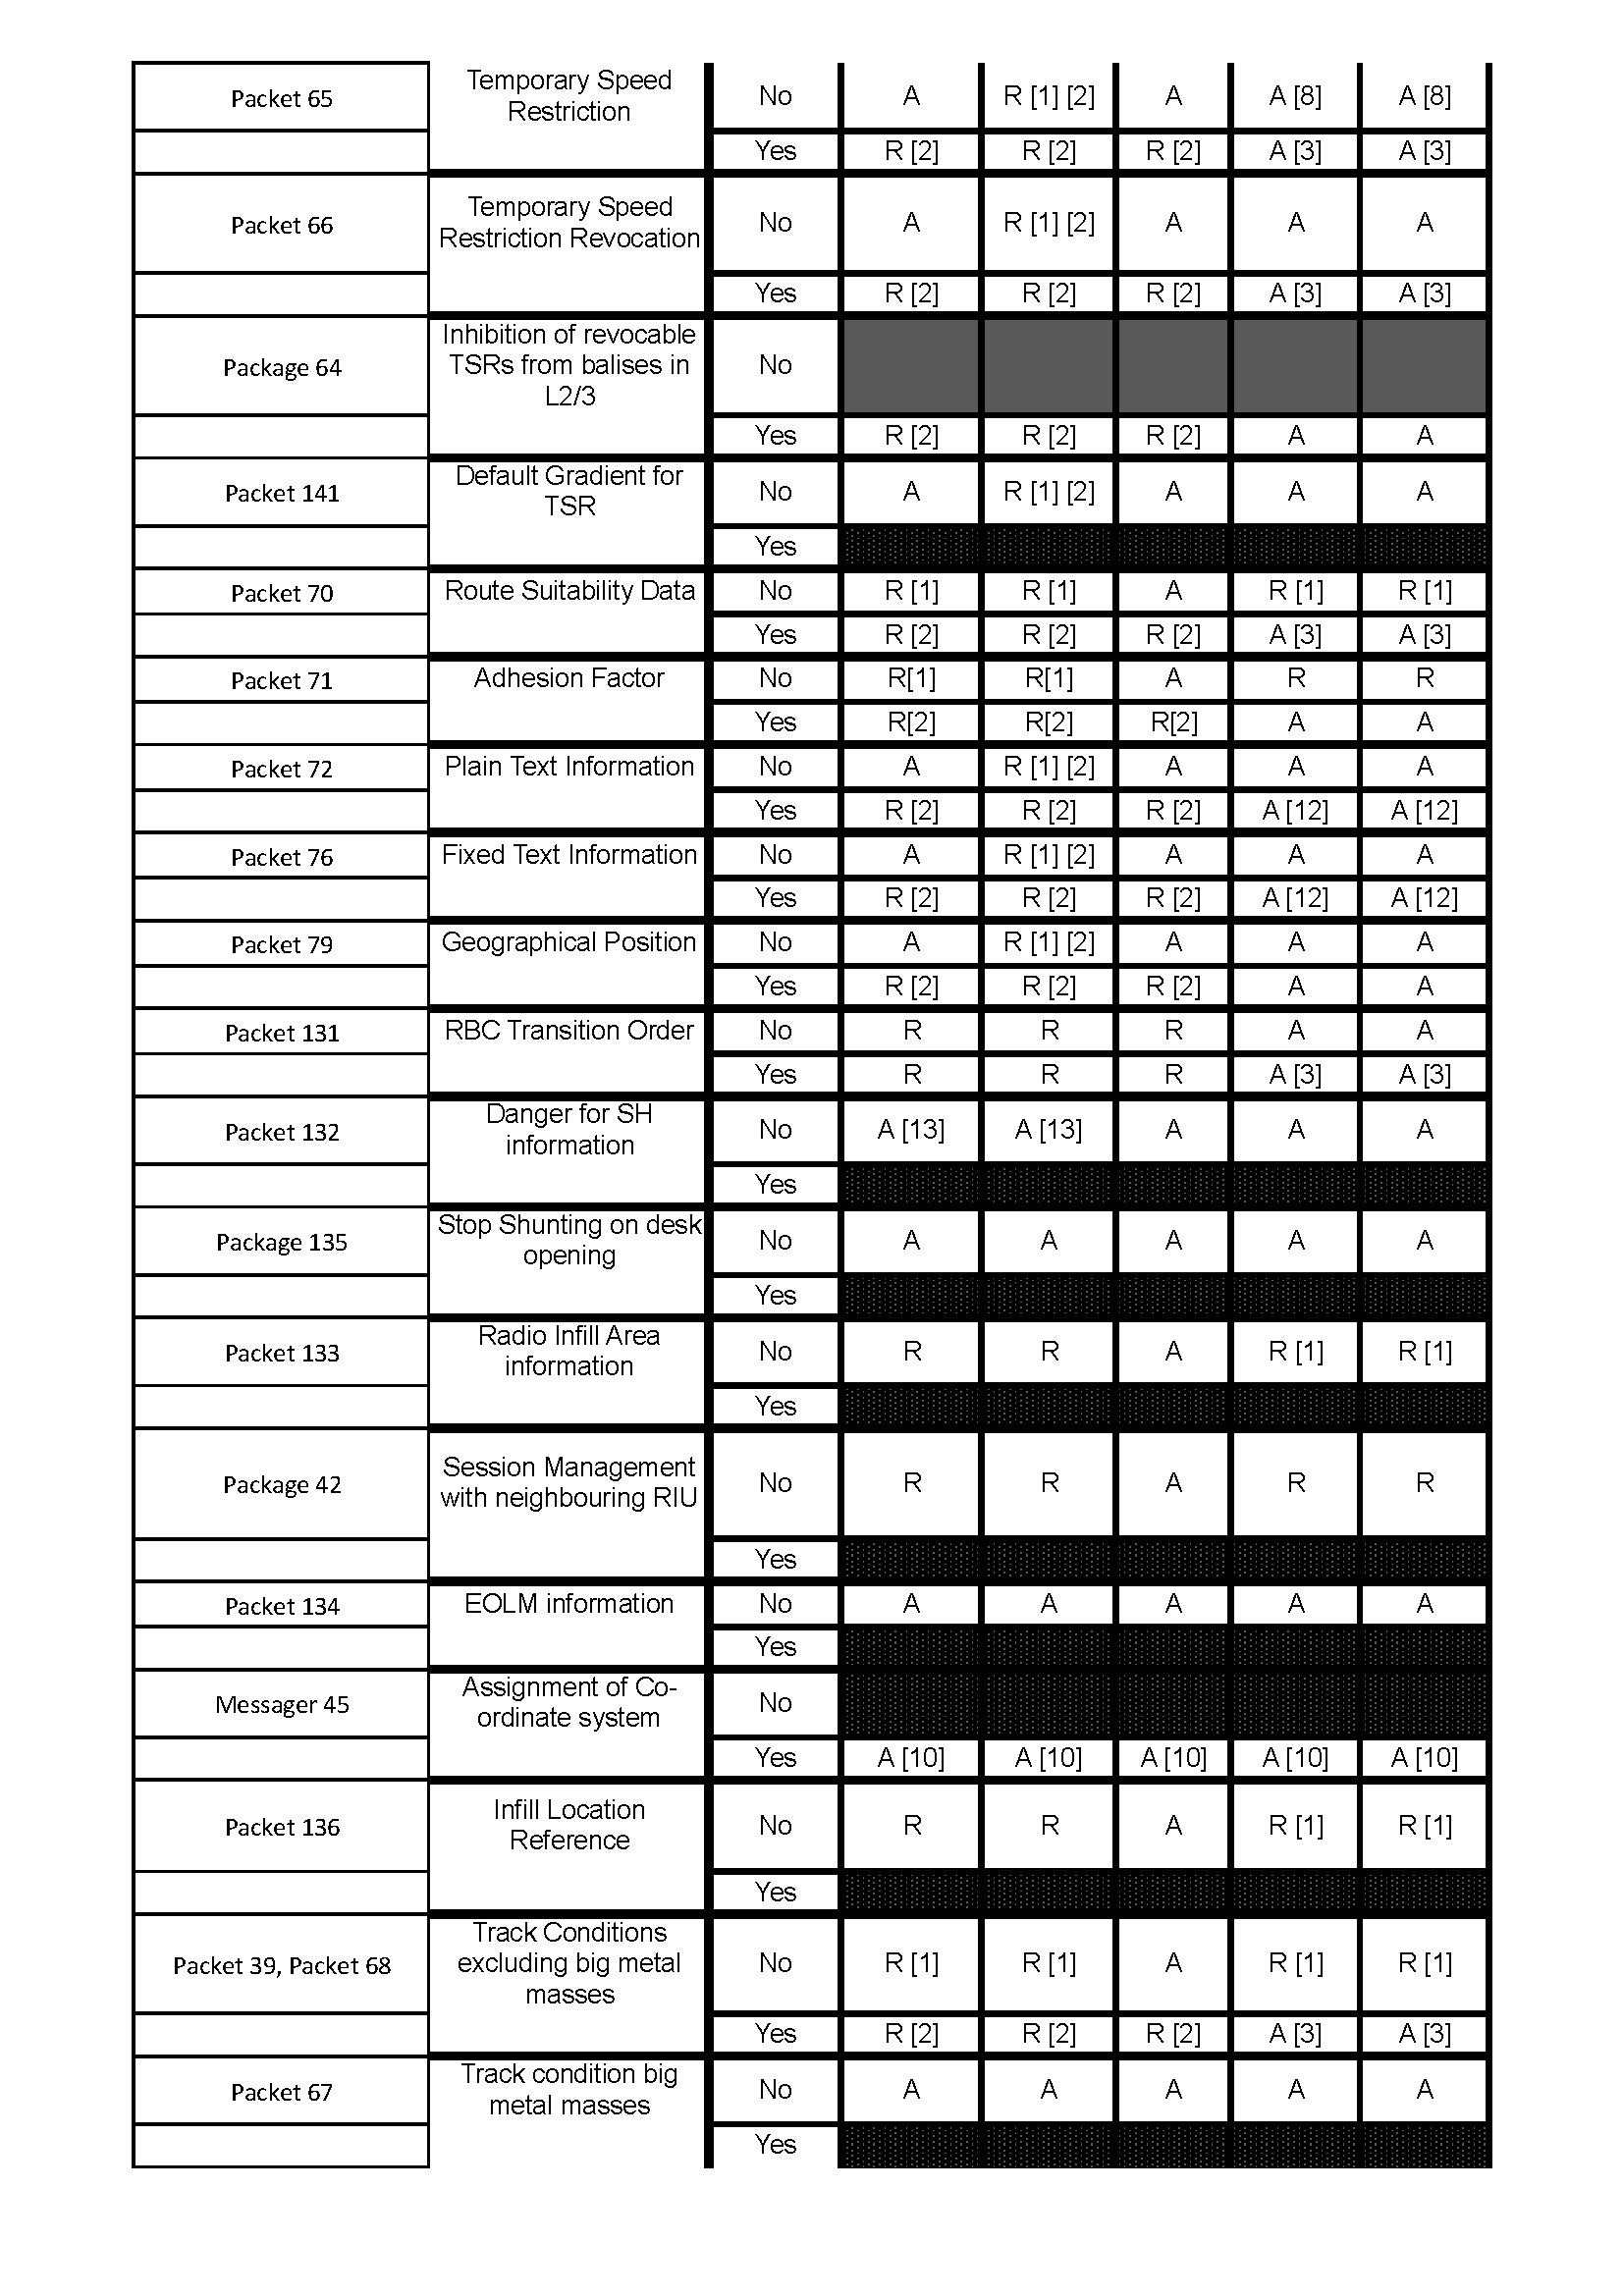
\includegraphics [scale=0.6]{images/LevelFilter2}
\end{figure}
\begin{figure}[hbtp]
\centering
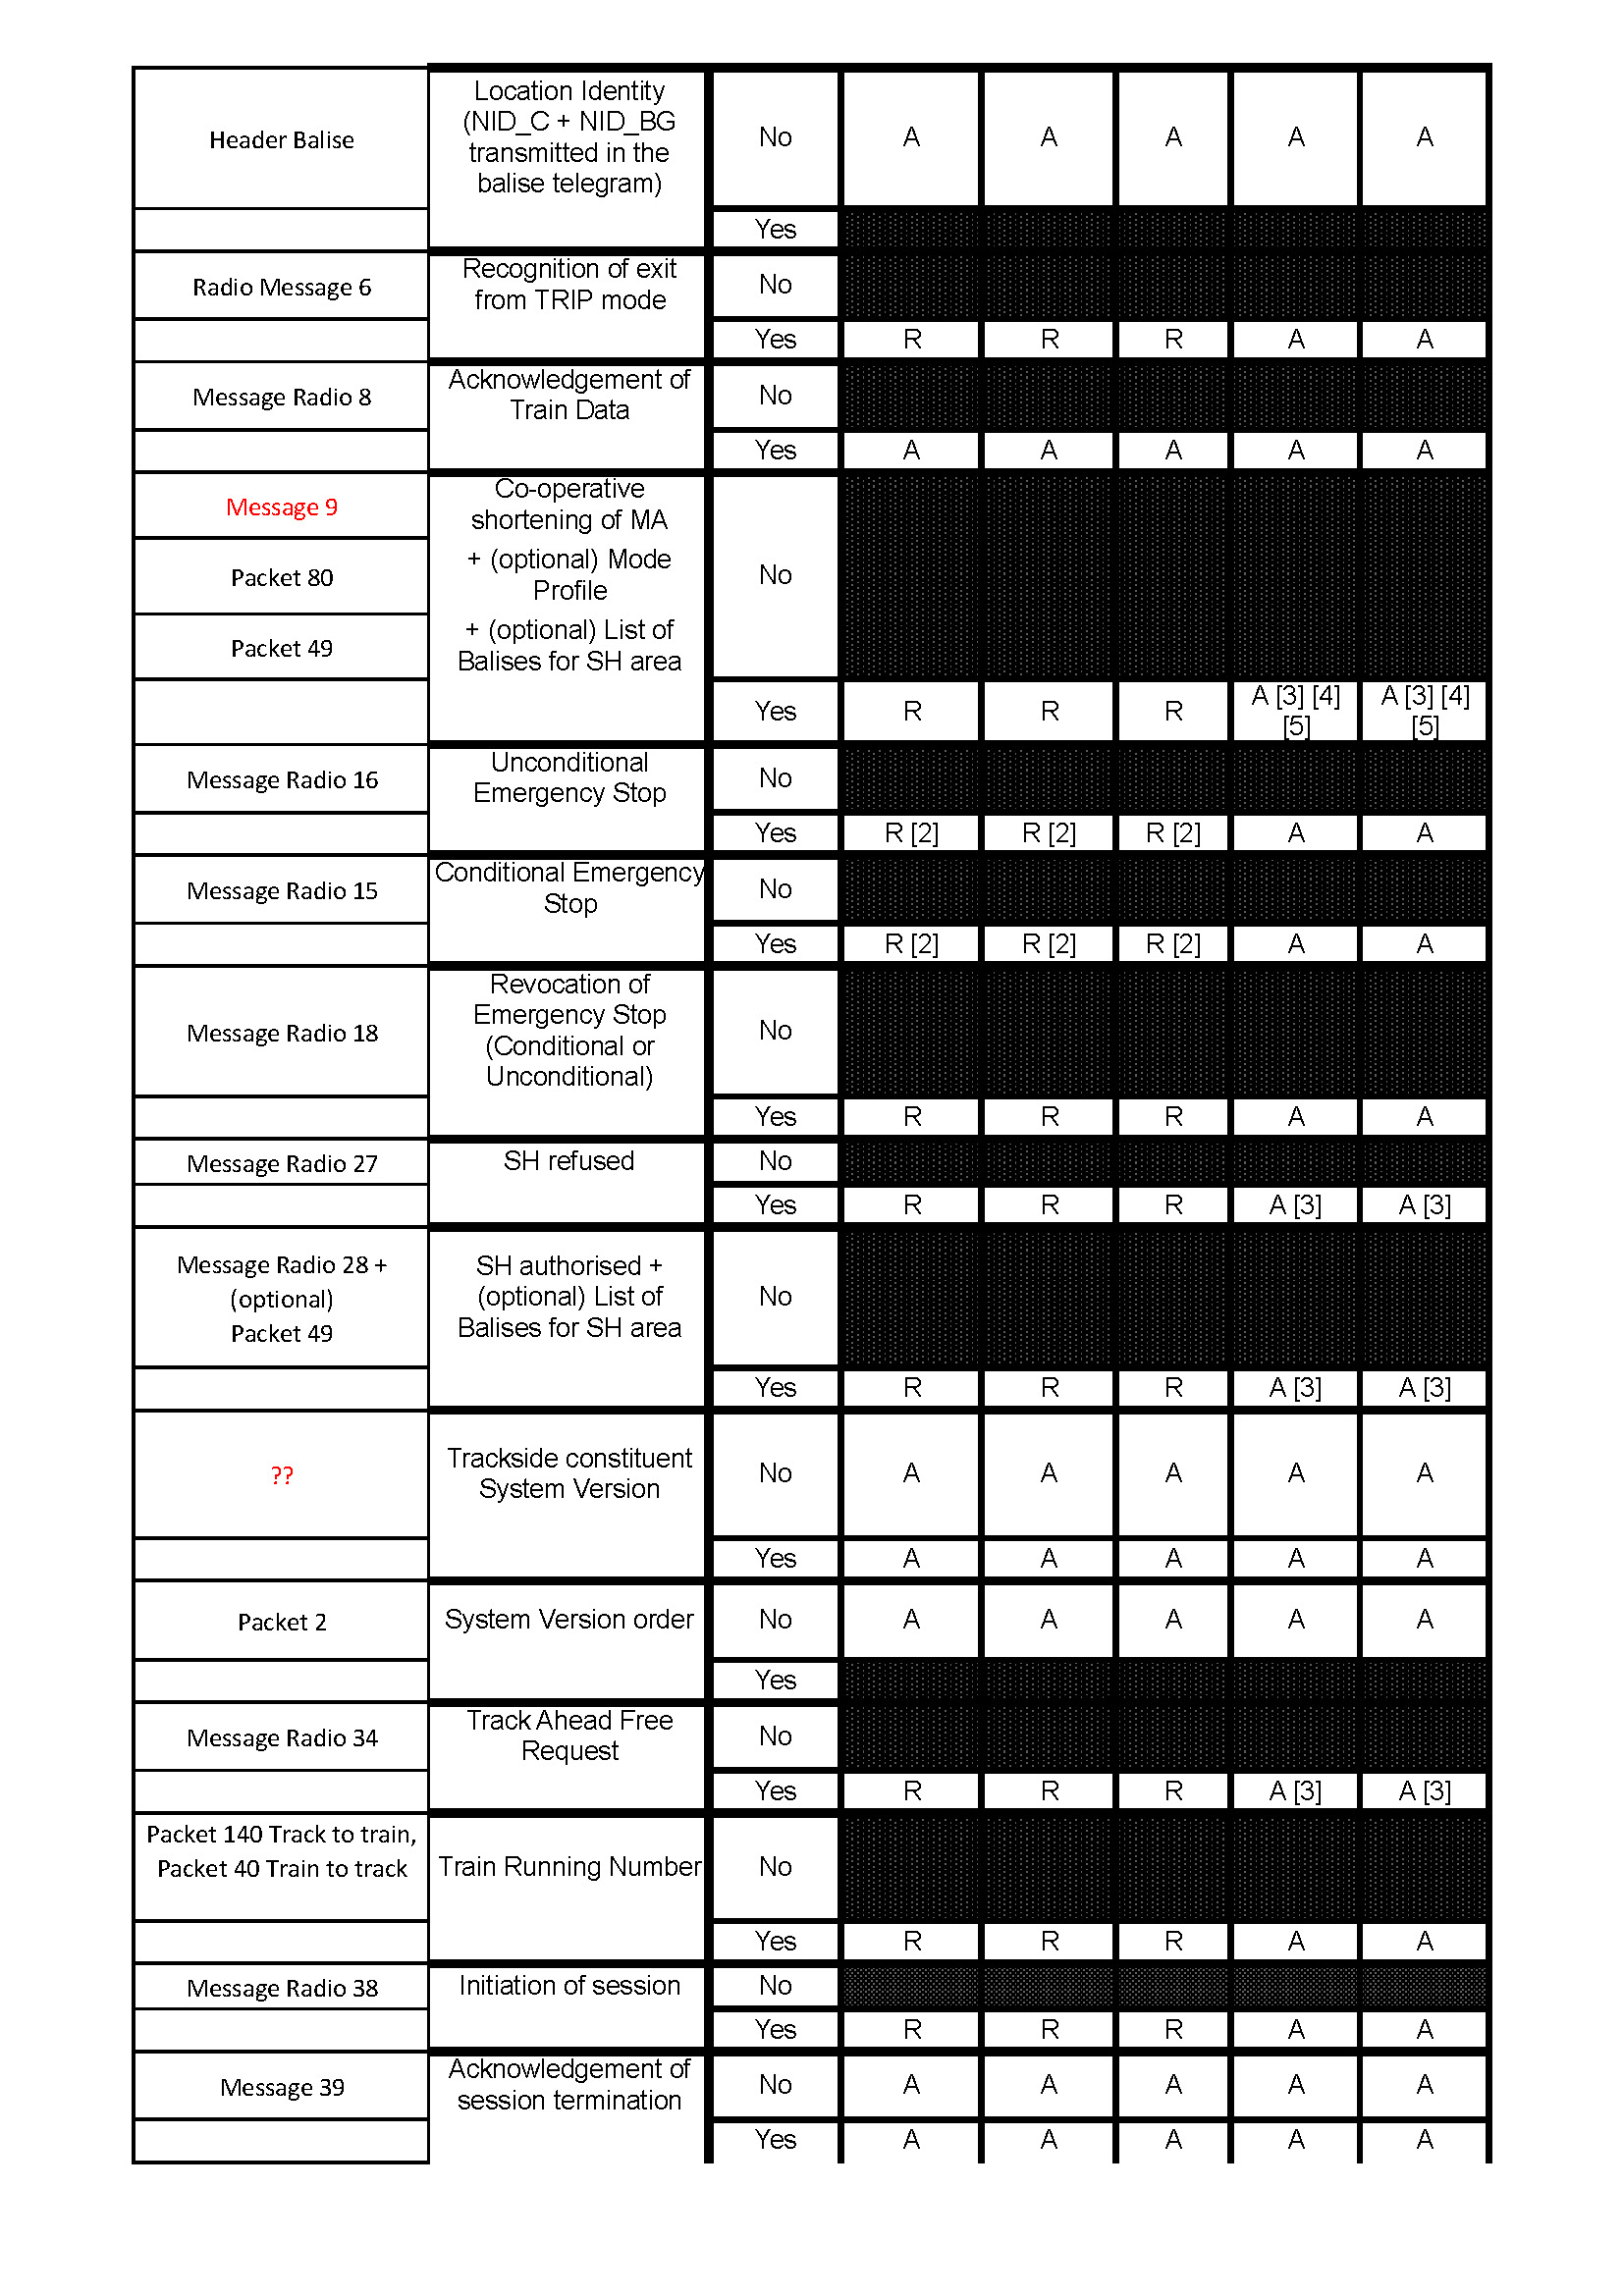
\includegraphics [scale=0.6]{images/LevelFilter3}
\end{figure}
\begin{figure}[hbtp]
\centering
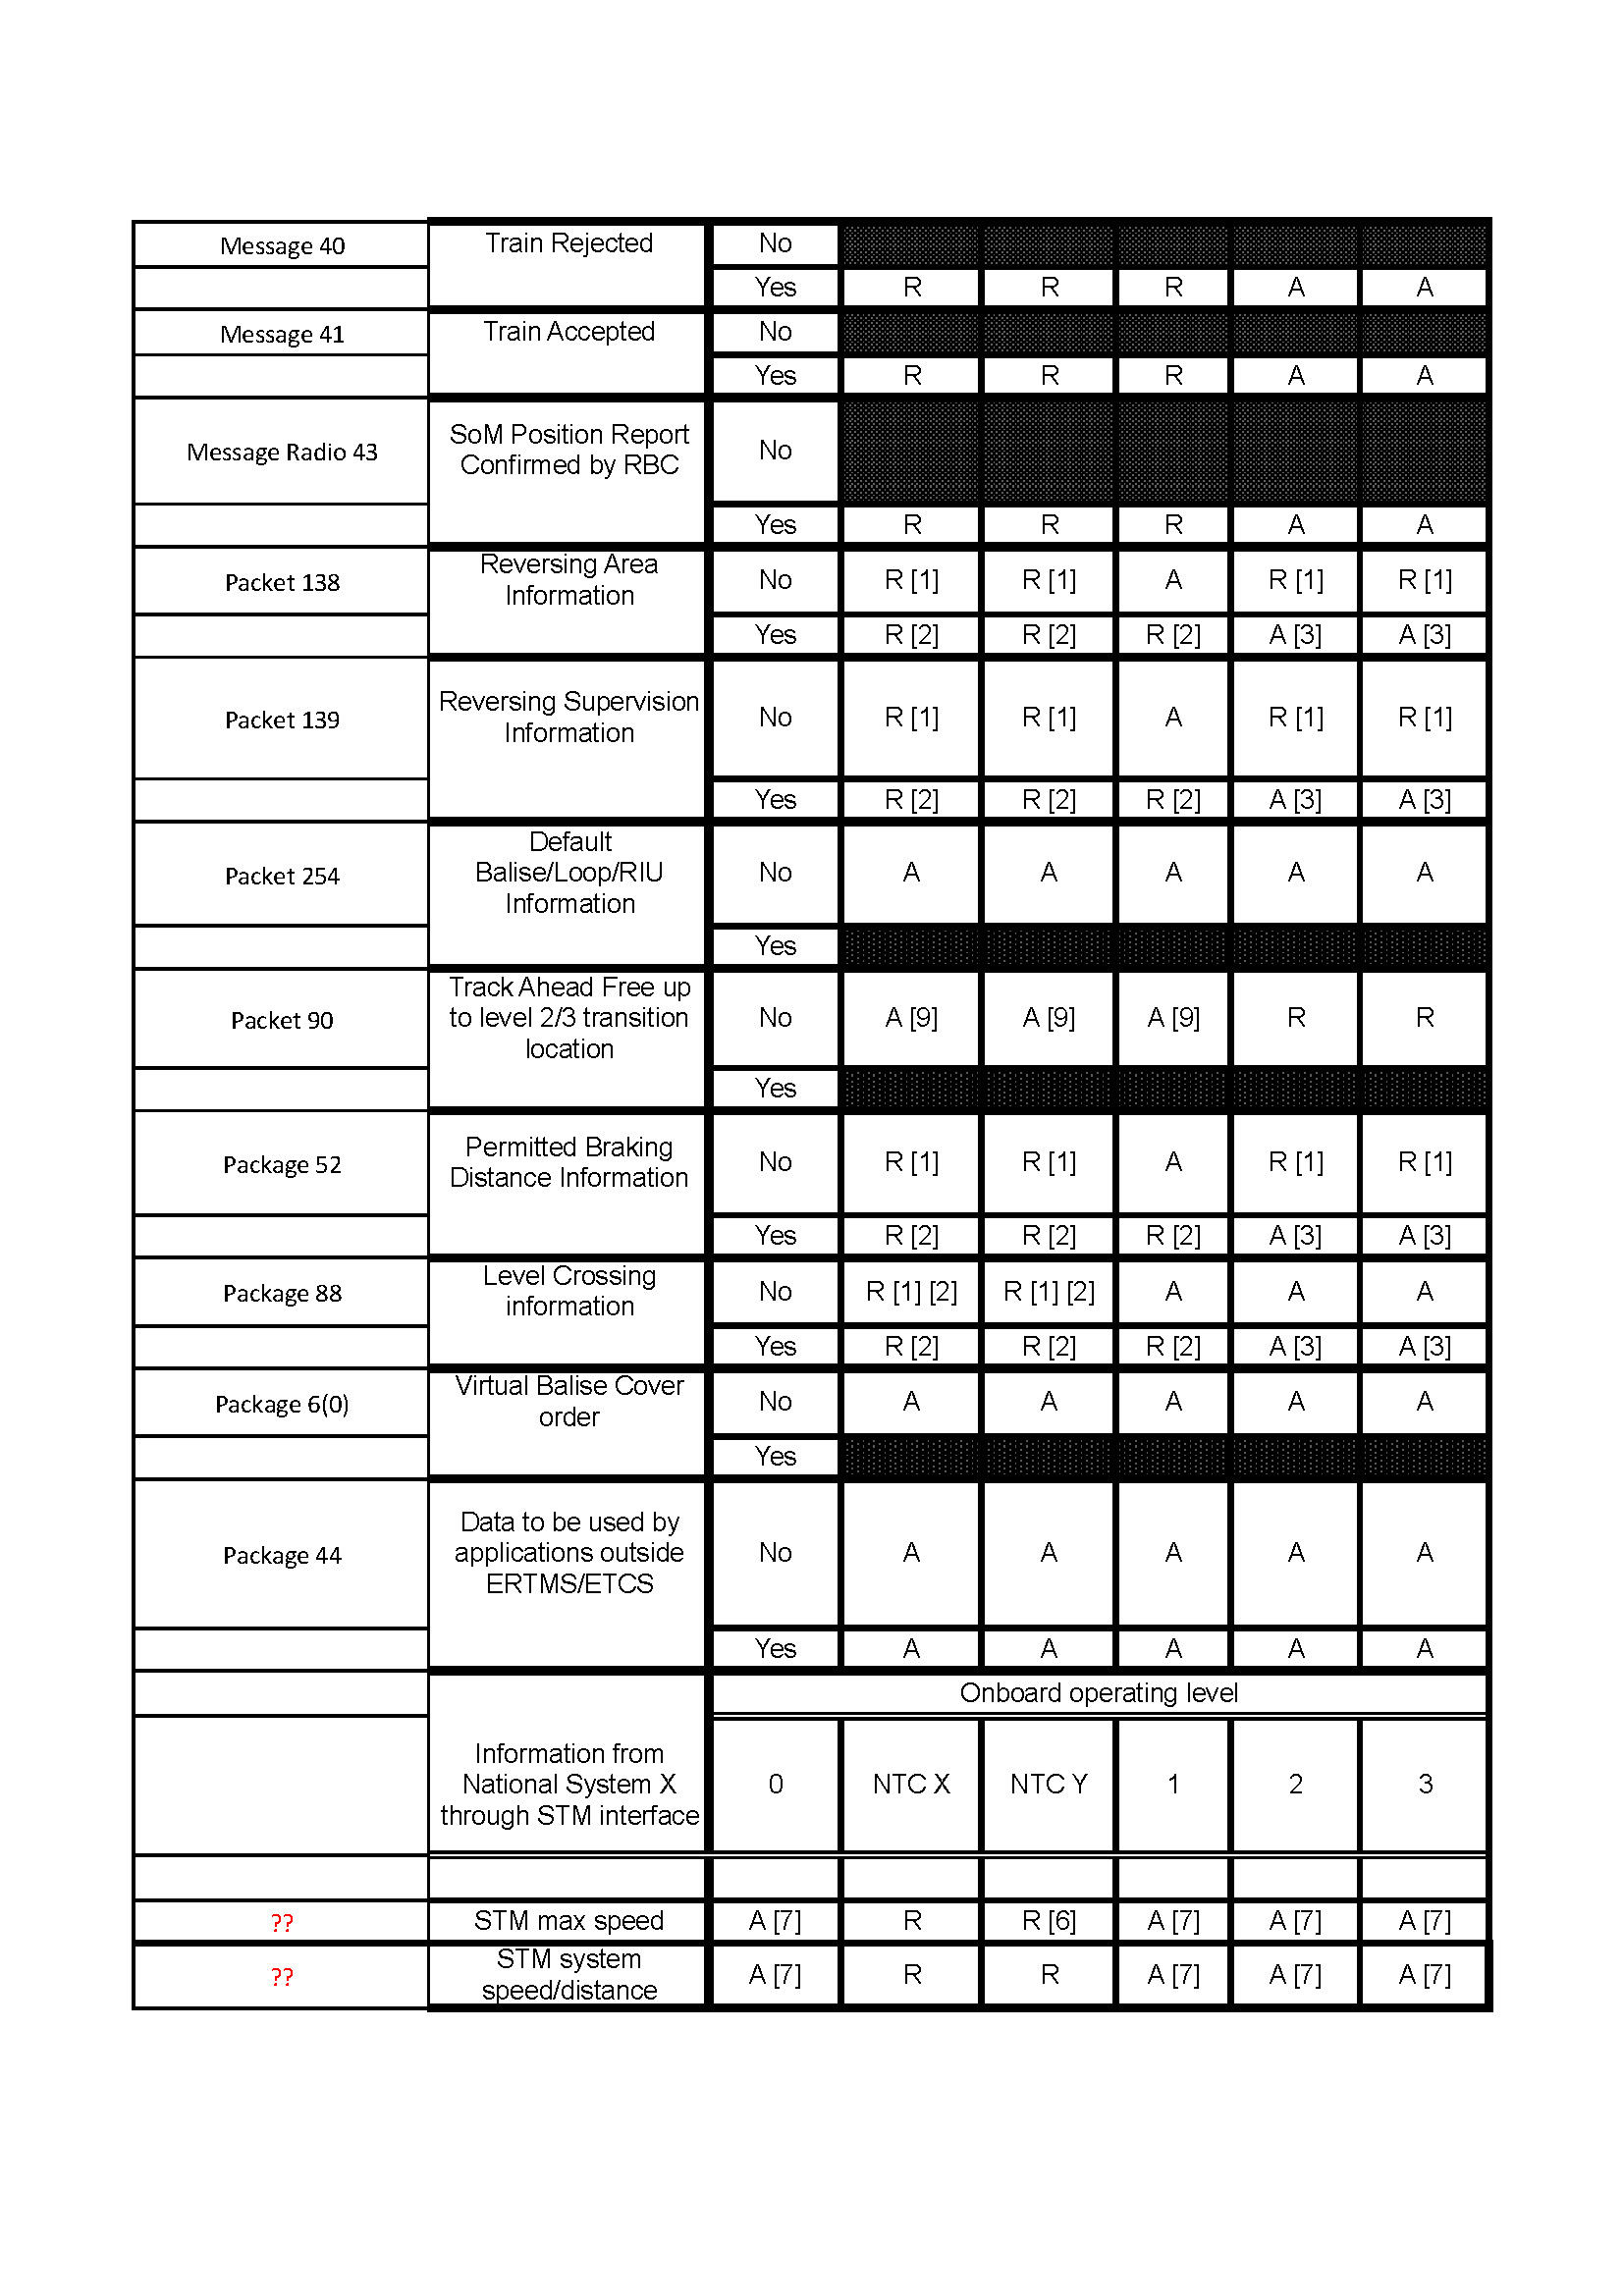
\includegraphics [scale=0.6]{images/LevelFilter4}
\caption{Lists of packages and their handling depending on train modes}
\label{fig:PackagesListLevel}
\end{figure}
\newpage

\begin{figure}[hbtp]
\centering
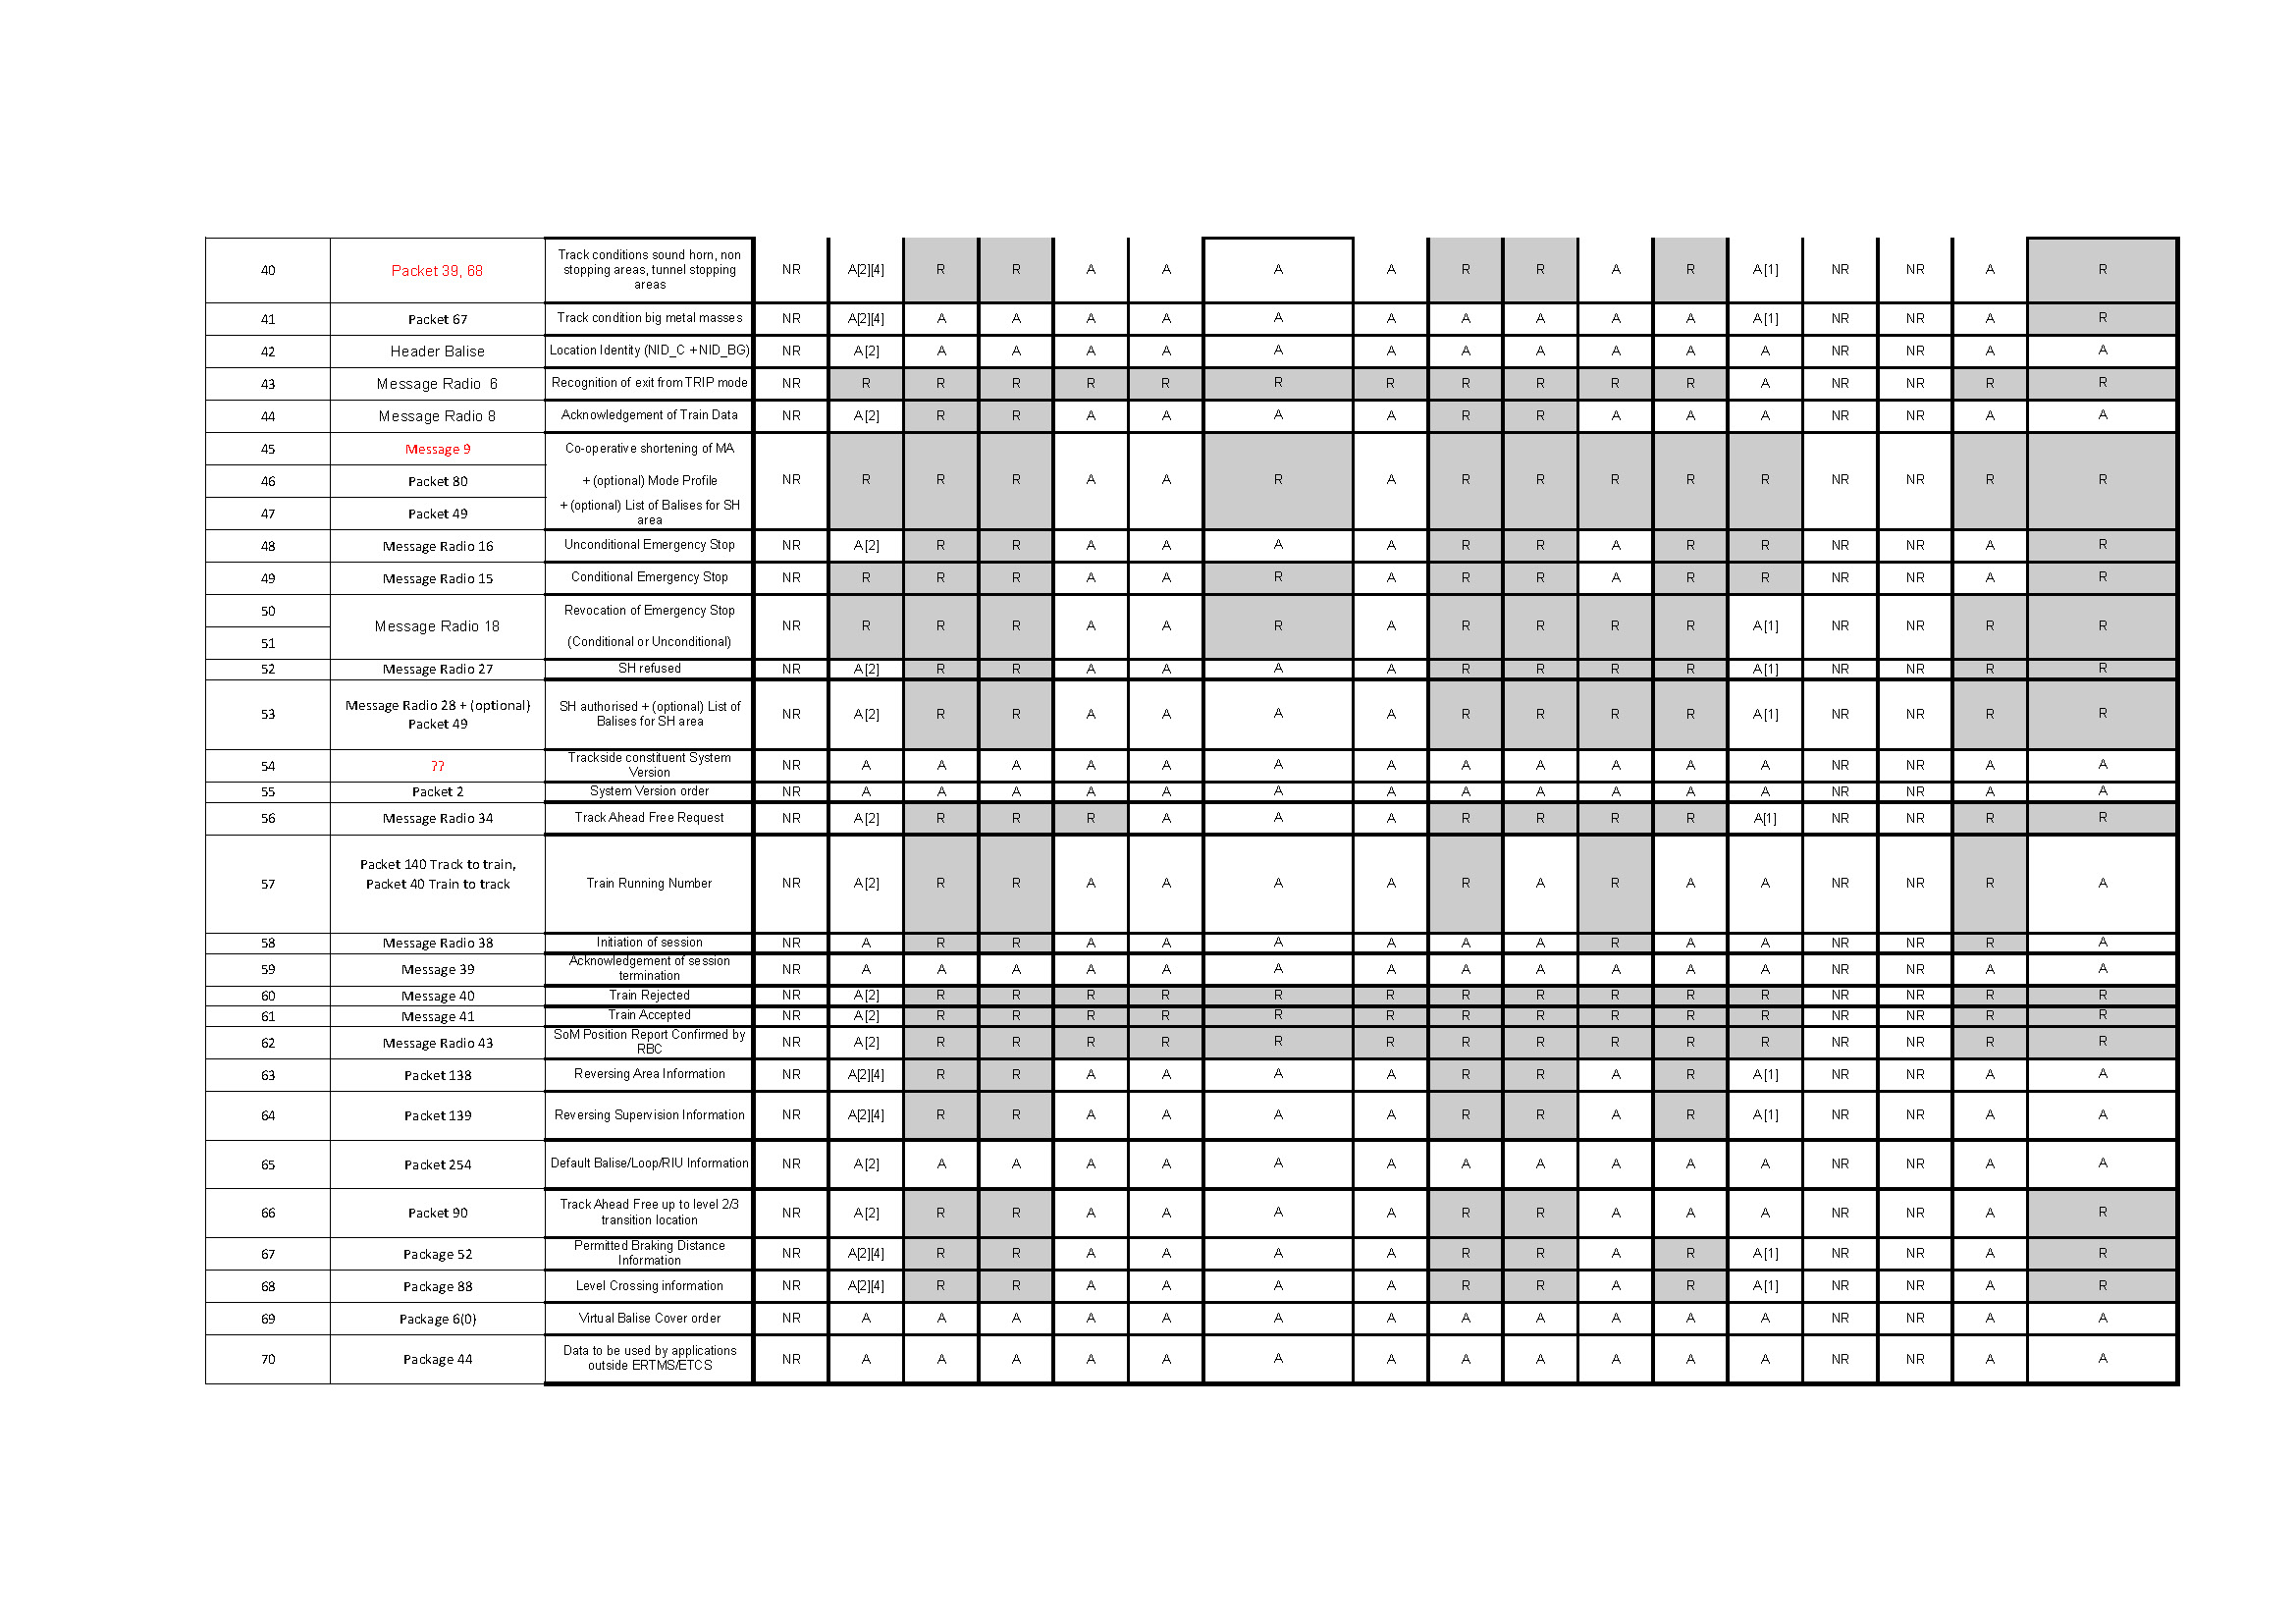
\includegraphics [angle=90, scale=0.8]{images/FilterMode1}
\end{figure}
\begin{figure}[hbtp]
\centering
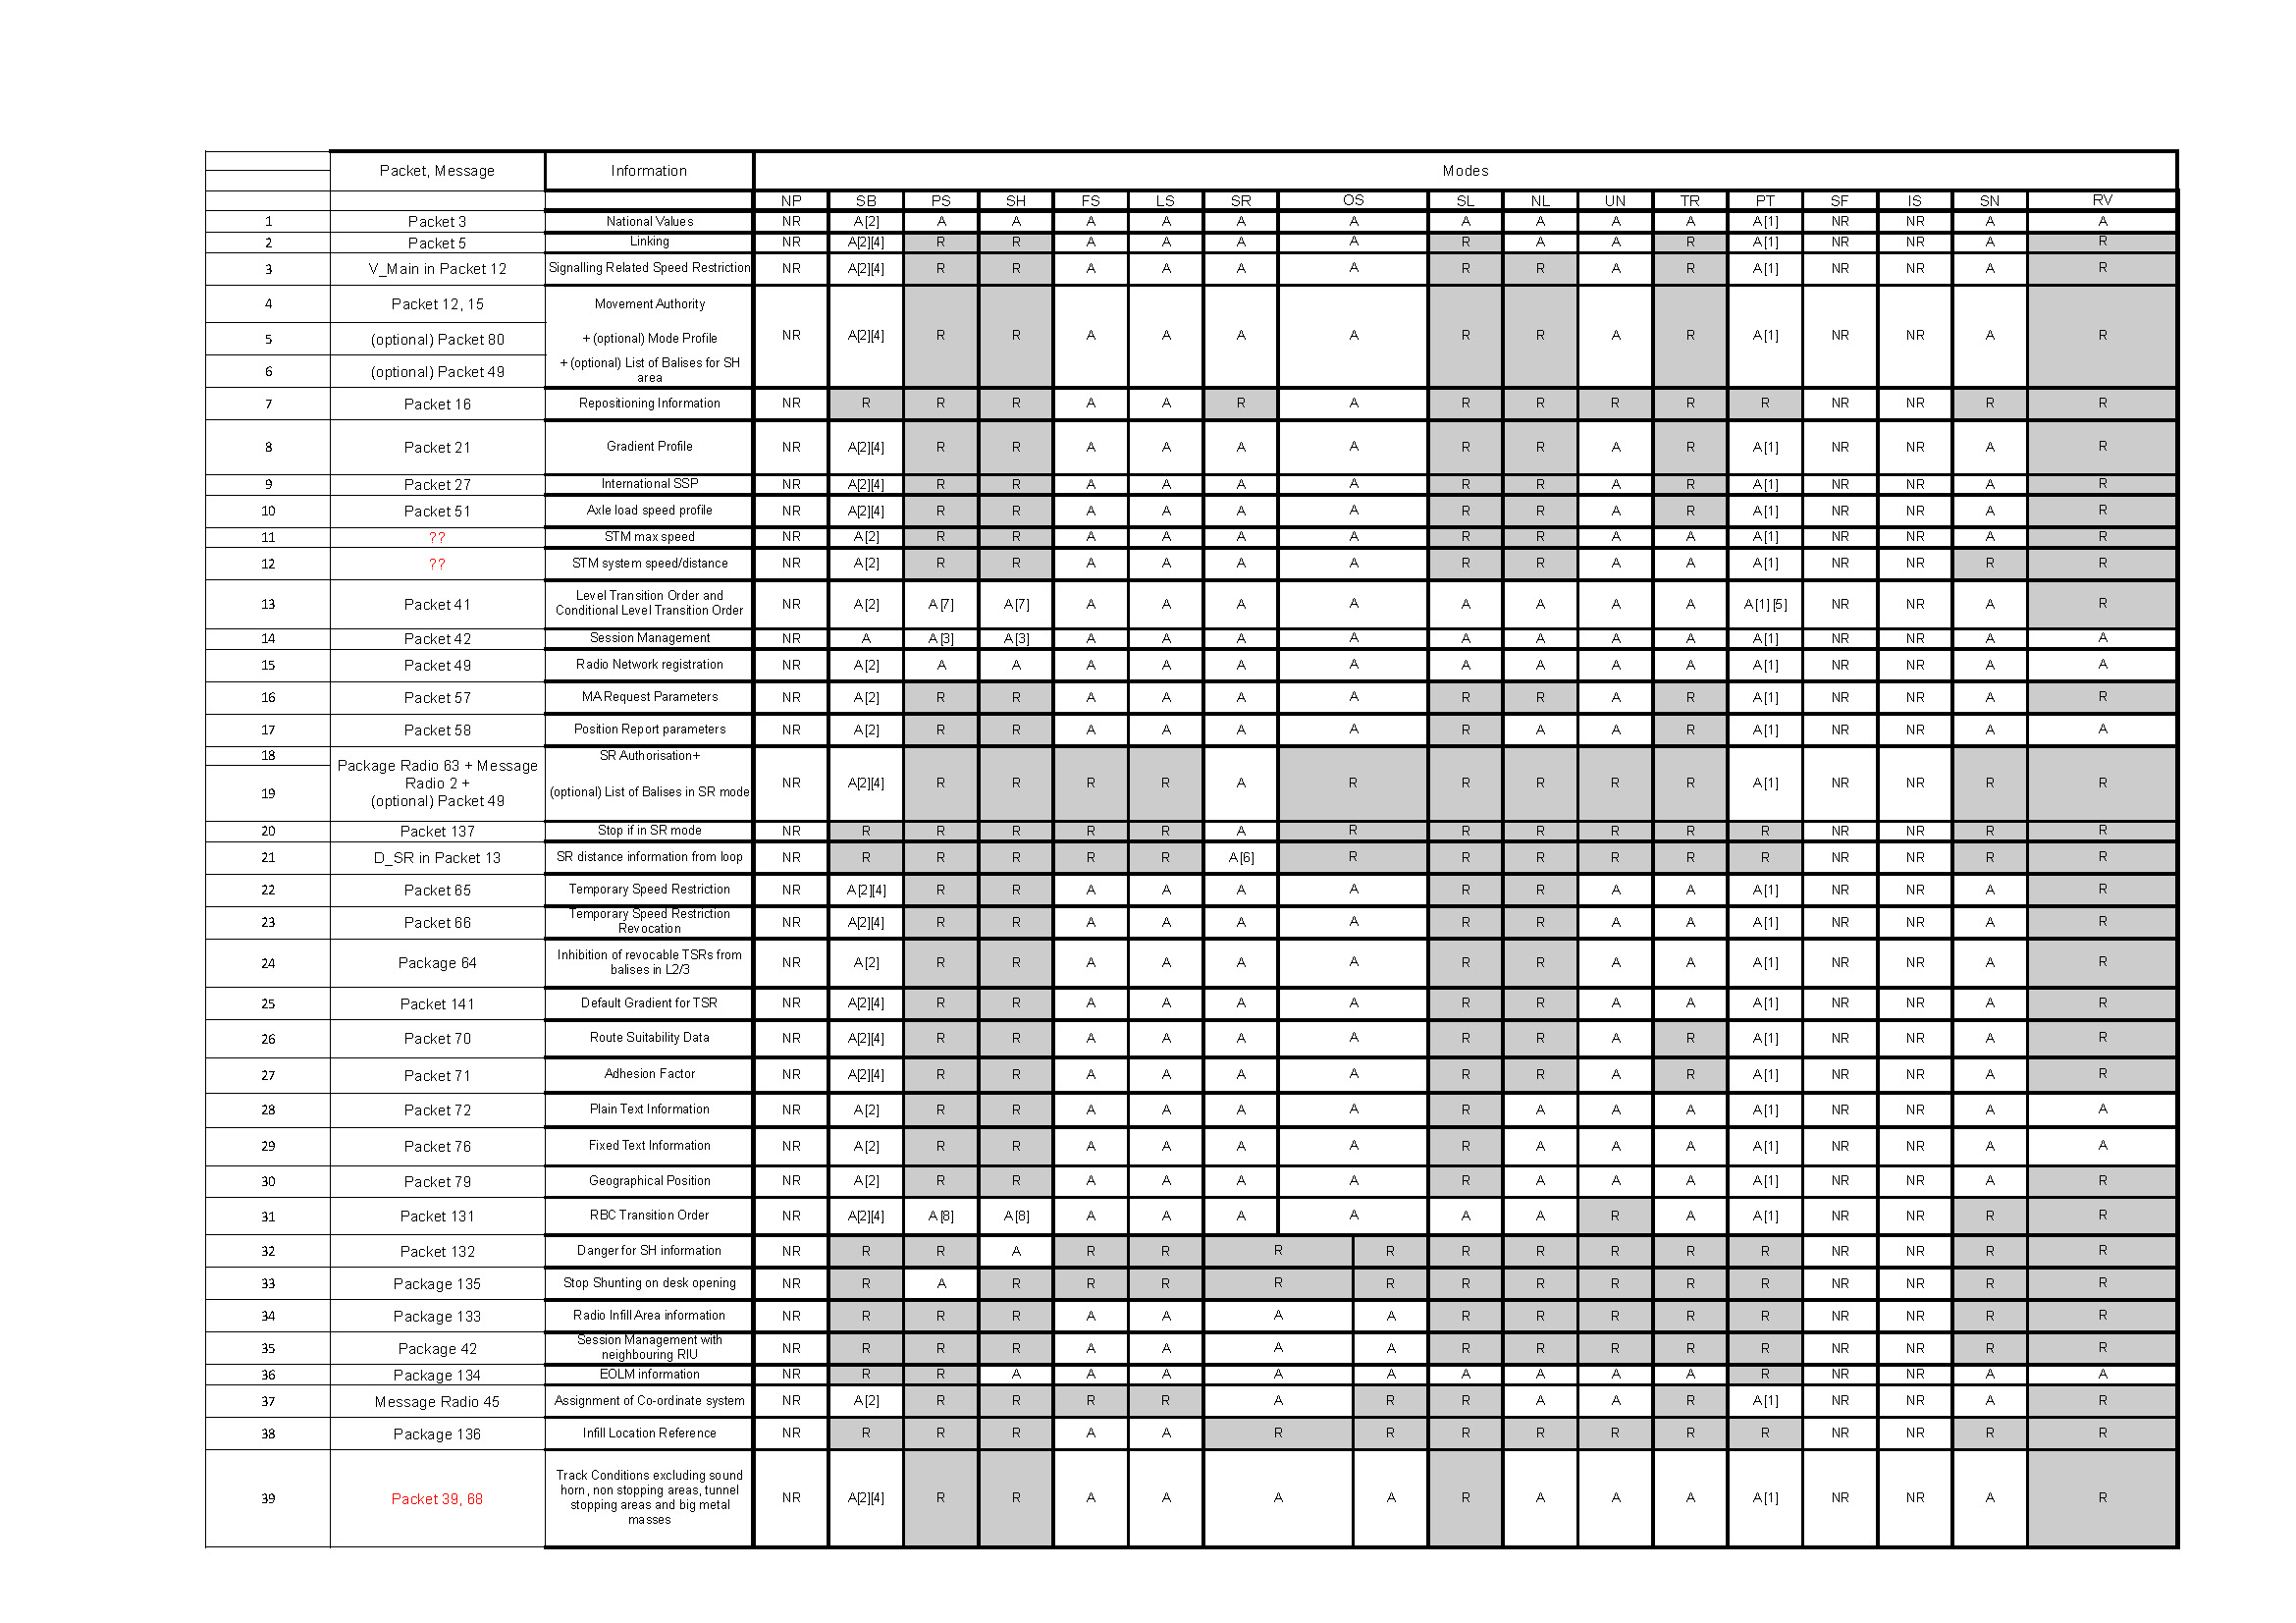
\includegraphics [angle=90, scale=0.8]{images/FilterMode2}
\end{figure}
\begin{figure}[hbtp]
\centering
\caption{Lists of packages and their handling depending on train modes}
\label{fig:PackagesListMode}
\end{figure}
\newpage

%%\subparagraph{Filtering (Mode/Level) - One packet per type}
%%\textbf{ISSUE: HOW MANY PKT 44, 65 AND 66 PER MESSAGE ARE MAXIMALLY SUPPORTED? (BH: who made this comment??)}\\

%% - Check on announced and immediate level transition orders in the messages to be filtered (needed for further criteria for filtering, to decide if the data shall be stored in the transition buffer).\\
%% - Filter data stored in the transition buffer according to the current level (what to do if similar information is available in the new message??). Data can be rejected, accepted or kept in the transition buffer.
%% (Filtering according to new level will be done directly afterwards in the next cycle)\\
%% - Filter new received messages according to the current level (new level will be done in the next cycle as according to \gls{SRS} data first has to be filtered according to old level and afterwards to new level). Data can be rejected, accepted or stored in the transition buffer.\\
%% - Filter (level) accepted data according to originating RBC (supervising or other). Information from \gls{BG}'s, loops or RIU is not filtered with this filter.\\
%% - Filter (level and RBC) accepted data according to the current mode (only reject or accept)\\


\paragraph{Reference to the Scade Model}
The SCADE model can be found on github under the following path:

\tiny\url{https://github.com/openETCS/modeling/tree/master/model/Scade/System/ObuFunctions/ManageLocationRelatedInformation/BaliseGroup/InformationFilter}
\normalsize

%set the master document for easy compilation
%!TEX root = ../D3_5_2.tex

%-----------------------------------------------------------------------
\section{Train Supervision}
%-----------------------------------------------------------------------
%\tbc
%Group 1 (Christian Stahl)

\begin{figure}
\centering
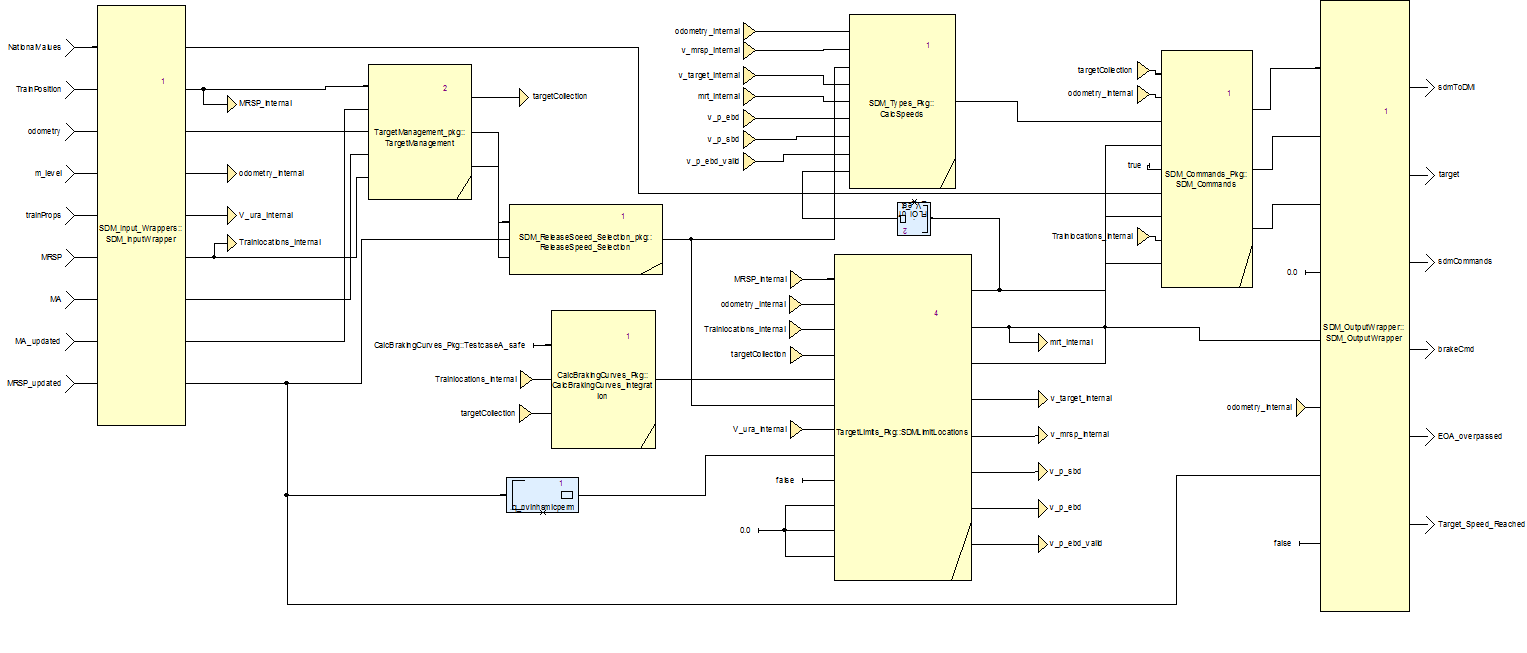
\includegraphics[width=0.95\textheight, angle=90]{../images/speedsupervision.png}
\caption{Structure of component ProvidePositionReport}\label{fig:ssv}
\end{figure}

The task of block ``Train Supervision'' is to monitor the speed of the train and the train location and as such to ensure that the speed remains within the given speed and distance limits. This block is mainly based on \cite[Chapt.~3.13]{subset-026}.

The block ``Train Supervision'' takes as input (1) movement related information such as train speed, train position and acceleration, (2) train related information such as brake information and train length, and (3) track related information such as speed and distance limits and national values.

Based on this information a speed profile is calculated. Speed restrictions create target speeds (targets) that have to be followed. For each such target braking curves are generated to supervise at which location of the track the train must perform the brake. In case of no target restrictions the train may accelerate to the supervised maximum speed of the speed profile. These calculations lead to commands being sent to the driver and the brake system.

The functionality is modeled using eight operators, as shown in Figure~\ref{fig:ssv}, which are explained below.

The current status of the analysis of ``Train Supervision'' and a functional breakdown can be found in a separate document, \verb+SpeedSupervision_analysis.pdf+.



\subsection{Input}
For providing the output, the module needs different input data flows. Table \ref{tbl:speedsupervisionInput} gives an overview.

\begin{table}[H]
  \begin{tabular}{| c | l | l | l | l |}
    \hline
    \textbf{Index} & \textbf{Input name} & \textbf{Input type} & \textbf{Source}\\ \hline
    0 & \texttt{NationalValues} & \texttt{P3\_NationalValues\_T} & ???\\
    1 & \texttt{TrainPosition} & \texttt{trainPosition\_T} & Manage Track Data\\
    2 & \texttt{odometry} & \texttt{odometry\_T} & Odometry\\
    3 & \texttt{m\_level} & \texttt{M\_LEVEL} & Mode and Level\\
    4 & \texttt{trainProps} & \texttt{trainProperties\_T} & Database\\
    5 & \texttt{MRSP} & \texttt{MRSP\_Profile\_t} & ?? \\
    6 & \texttt{MA} & \texttt{MAs\_t} & ??\\
    7 & \texttt{MA\_updated} & \texttt{bool} & internal\\
    8 & \texttt{MRSP\_updated} & \texttt{bool} & internal\\
    \hline
  \end{tabular} 
  \caption{Overview of inputs}
  \label{tbl:speedsupervisionInput}
\end{table}

\subsubsection{Input 0: \texttt{NationalValues}}
This input is packet 3 of \cite[Chapt.~8]{subset-026}, describing the national values. 
\subsubsection{Input 1: \texttt{TrainPosition}}
This input is the current train position.
\subsubsection{Input 2: \texttt{odometry}}
This input is the odometry data.
\subsubsection{Input 3: \texttt{m\_level}}
This input is the current level of the train.
\subsubsection{Input 4: \texttt{trainProps}}
This input is a set of train related properties.
\subsubsection{Input 5: \texttt{MRSP}}
This input is the most restrictive speed profile.
\subsubsection{Input 6: \texttt{MA}}
This input is a movement authority.
\subsubsection{Input 7: \texttt{MA\_updated}}
This flag is true if the movement authority has been updated in this clock cycle and false otherwise.
\subsubsection{Input 8: \texttt{MRSP\_updated}}
This flag is true if the most restrictive speed profile has been updated in this clock cycle and false otherwise.



\subsection{Output}
Based on the input the block produces the following output. Table~\ref{tbl:speedsupervisionOutput} gives an overview.

\begin{table}[H]
  \begin{tabular}{| c | l | l | l |}
    \hline
    \textbf{Index} & \textbf{Output name} & \textbf{Output type}\\ \hline
    0 & \texttt{sdmToDMI} & \texttt{speedSupervisionForDMI\_T}\\
    1 & \texttt{target} & \texttt{Target\_T}\\
    2 & \texttt{sdmCommands} & \texttt{SDM\_Commands\_T}\\
    3 & \texttt{brakeCmd} & \texttt{Brake\_command\_T}\\
    4 & \texttt{EOA\_overpassed} & \texttt{bool}\\
    5 & \texttt{Target\_Speed\_Reached} & \texttt{bool}\\
    \hline
  \end{tabular} 
  \caption{Overview of outputs}
  \label{tbl:speedsupervisionOutput}
\end{table}

\subsubsection{Output 0: \texttt{sdmToDMI}}
This output contains information about different speeds and positions, on the one hand and the current supervision status, on the other hand. This information shall be displayed to the driver.
\subsubsection{Output 1: \texttt{target}}
This output is the most restrictive displayed target (MRDT).
\subsubsection{Output 2: \texttt{sdmCommands}}
This output gives some intermediate results of operator SDM\_Commands. It is currently used for test purposes only.
\subsubsection{Output 3: \texttt{brakeCmd}}
This output is the brake command, indicating whether performing the service brake or the emergency brake have been commanded.
\subsubsection{Output 4: \texttt{EOA\_overpassed}}
This output is true if the end of authority has been overpassed and false otherwise.
\subsubsection{Output 5: \texttt{Target\_Speed\_Reached}}
This output is true if the current speed is greater than or equal the target speed and false otherwise.



\subsection{SDM\_InputWrapper in Train Supervision}

\subsubsection{Reference to the SRS or other Requirements (or other requirements)}
\begin{itemize}
	\item \cite[Chapt.~3.13]{subset-026}: Speed and distance monitoring 
\end{itemize}

\subsubsection{Short description of the functionality}
The motivation for this operator is to convert all inputs of block ``Speed Supervision'' that contain information about length, speed, distance, and acceleration defined as integer into \texttt{real} to allow automatically the highest precision in the calculations by the meaning of floating point operations. In addition, to ease the modeling, inside block ``Speed Supervision'' only units meters ($[m]$), seconds($[s]$), meters per second($[\frac{m}{s}]$), and meters per square second($[\frac{m}{s^{2}}]$) are used.

\subsubsection{Interface}

\subsubsection{Functional Design Description}
This operator forwards input messages, takes data from complex data types or transforms inputs messages into an internal type thereby converting int to real.
  
\subsubsection{Reference to the Scade Model}

\subsection{TargetManagement in Train Supervision}

\subsubsection{Reference to the SRS or other Requirements (or other requirements)}
\begin{itemize}
	\item \cite[Chapt.~3.13.8.2]{subset-026}: Determination of the supervised targets 
\end{itemize}

\subsubsection{Short description of the functionality}
This operator calculates/updates the list of targets to be supervised by the block ``Train Supervision''. Taking the current movement authority, the most restrictive speed profile and the current maximum safe front end position as an input, the operator outputs a single End of Authority target, a list of all MRSP-Targets and a list of all LoA-Targets.
  
\subsubsection{Interface}

\subsubsection{Functional Design Description}
\paragraph{Derivation of Targets from Movement Authority Sections}
The sections of the \emph{Movement Authority} could cause two types of targets:
\begin{description}
\item[End Of Authority(EoA)] only one could exist and this is only in the \emph{end section} of the \emph{MA}
\item[Limit of Authority (LoA)] is possibly in every section of the \emph{MA} except the end section
\end{description}
In every cycle in which the MA is updated, the operator iterates through the entire MA and puts all speed limitations by \emph{LoA}s into a list of targets. The end section is used to derived the \emph{EoA} target. All LoA targets are sorted by location.

\paragraph{Derivation of Targets from MRSP}
According to \cite[Chapt.~3.13.8.2]{subset-026}, every speed decrease of the MRSP is used to derive a target. Therefore in every cycle in which the MRSP is updated, the operator iterates through the entire MRSP searching for all MRSP targets. For this purpose, every element of the MRSP is compared with its successor.

\paragraph{Update of Targets}
In every cycle the operator monitors whether all targets are already passed. To this end, it iterates over the list of targets comparing the current max safe front end position with the target position.

 


\subsubsection{Reference to the Scade Model}


\subsection{CalcBrakingCurves\_Integration in Train Supervision}
\subsubsection{Reference to the SRS or other Requirements (or other requirements)}
\begin{itemize}
	\item \cite[Chapt.~3.13.8.3]{subset-026}: Emergency Brake Deceleration curves (EBD)
	%
	\item \cite[Chapt.~3.13.8.4]{subset-026}: Service Brake Deceleration curves (SBD)
	%
	\item \cite[Chapt.~3.13.8.5]{subset-026}: Guidance curves (GUI)
\end{itemize}

\subsubsection{Short description of the functionality}
For each type of target a certain braking curve has to be calculated. This curve enables proactive monitoring of the train's speed. A reverse lookup on this braking curve indicates, where the train has to start braking given the current speed. The braking curve does not depend on the actual train status. As a consequence the braking curve stays constant over time. As a legitimate simplification the calculation of the braking curve is not extended after the estimated front end position of the train has been passed.

\subsubsection{Interface}

\subsubsection{Functional Design Description}
The calculation of the braking curve takes the complex function $A_{\mathit{safe}}$ as an input, which describes the overall braking performance of the train in a speed and position dependent meaning. This two-dimensional function needs to be simplified for every target to get a function of position to speed. Each individual target has a position and a speed (a point in the distance speed plane) and is the starting point of the braking curve. The first step is to get the deceleration of the train at the target point from the $A_{\mathit{safe}}$-function. Afterward the calculation iterates through the $A_{\mathit{safe}}$-function until the current estimated front end position is reached. Two cases can be distinguished:
\begin{itemize}
\item a new distance step of $A_{\mathit{safe}}$ is reached
\item a new speed step of $A_{\mathit{safe}}$ is reached
\end{itemize}

Both cases are checked and the applicable one is used to calculate a new arc. Every arc of the braking curve consists of:
\begin{itemize}
\item the distance where the arc begins,
\item the speed at the point where the arc begins,
\item the deceleration for the whole arc.
\end{itemize}
An abstract overview of the calculation could be seen in Fig.~\ref{fig:bc_calc}.

\begin{figure}
\centering
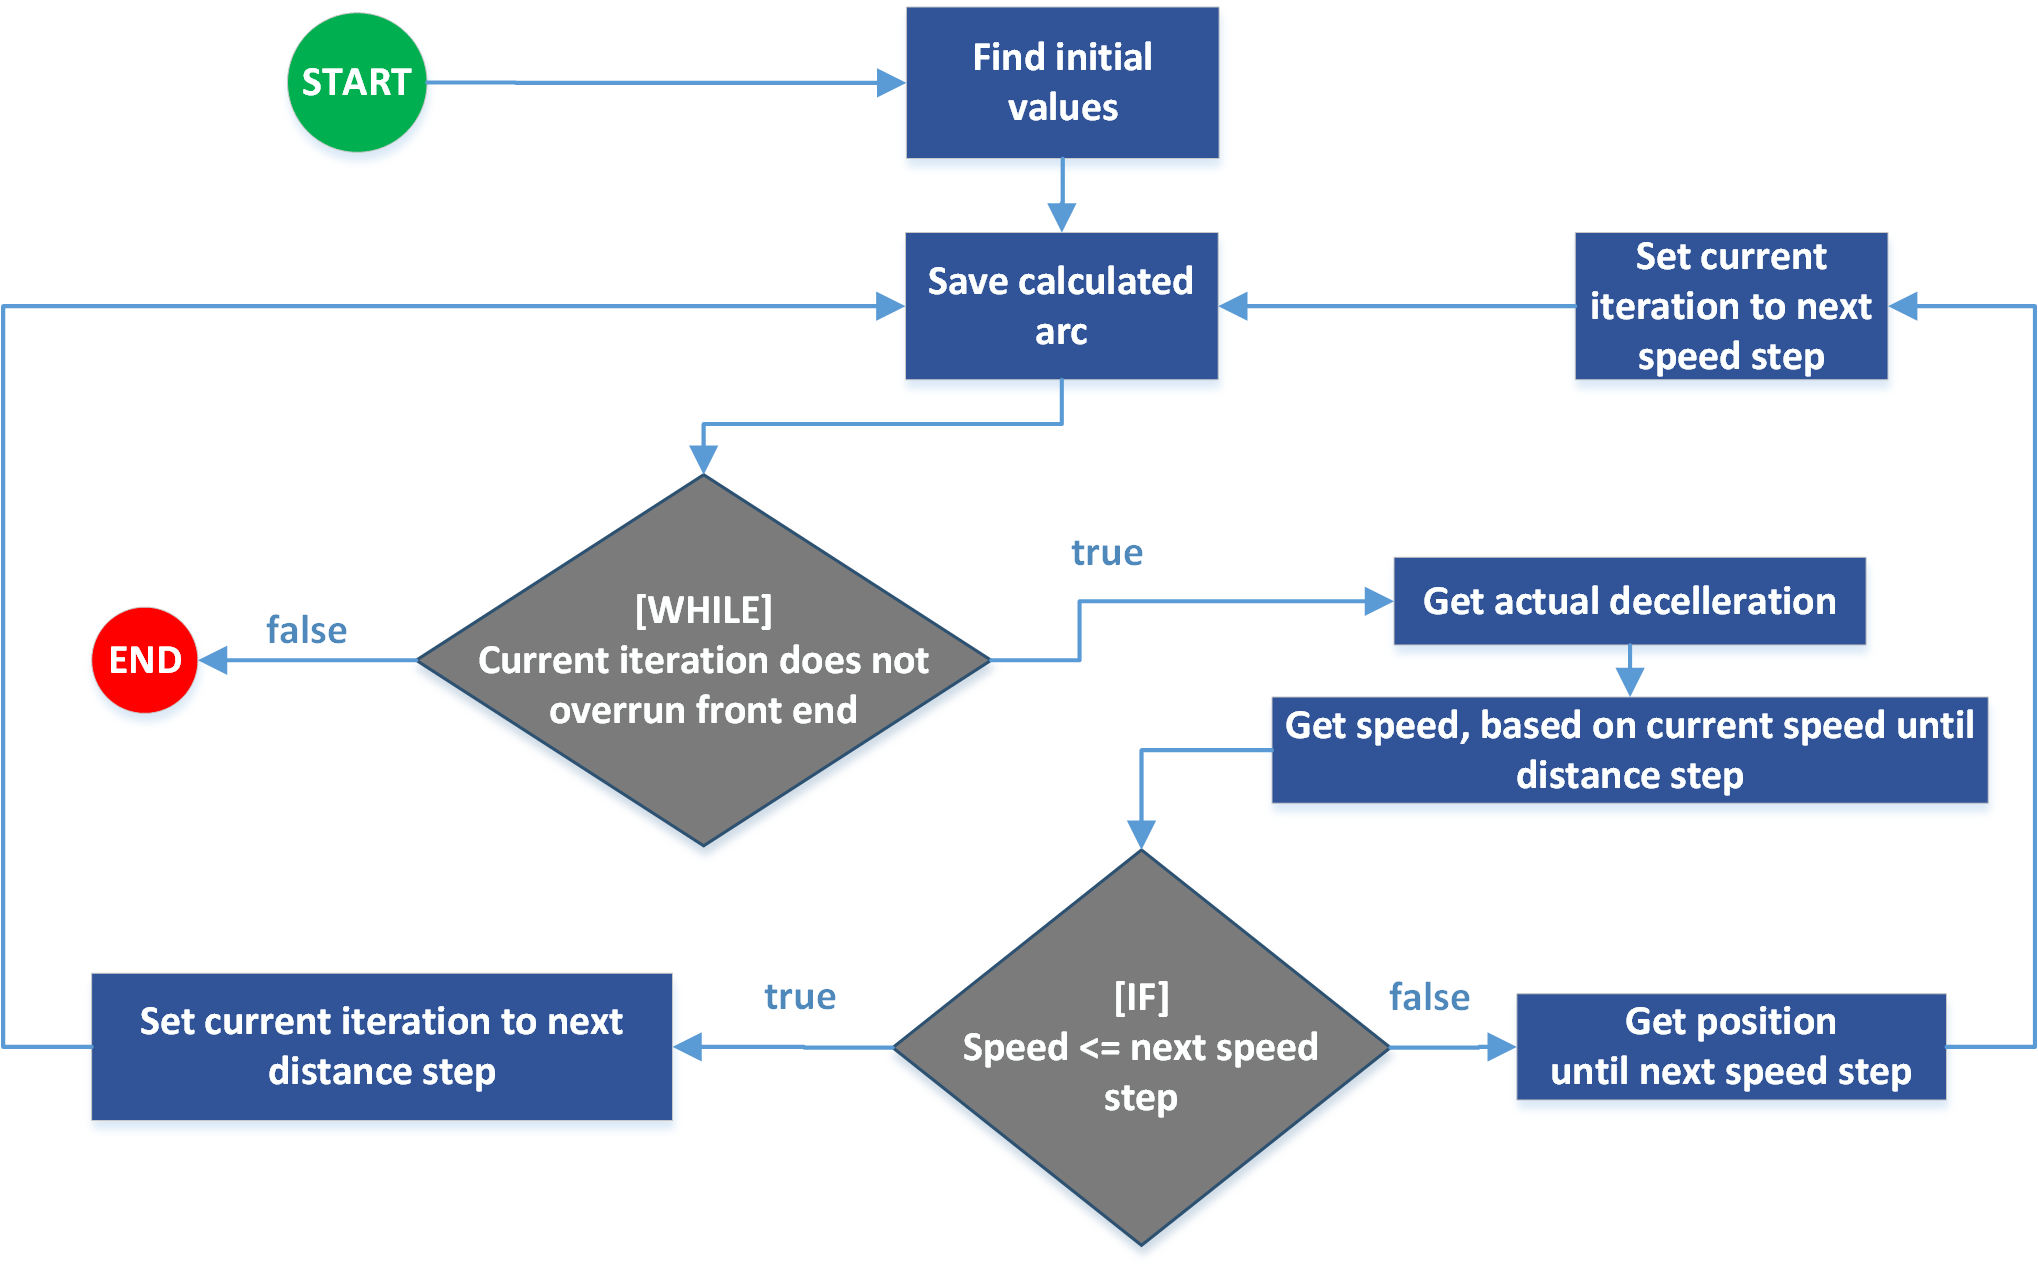
\includegraphics[width=0.95\textwidth]{../images/EBD_CalcAlgorithm.png}
\caption{Calculation of Braking Curves}\label{fig:bc_calc}
\end{figure}

Currently, the model supports the calculation of the following braking curves:
\begin{itemize}
	\item the Emergency Brake Deceleration curve for the most restrictive speed profile,
	%
	\item the Emergency Brake Deceleration curve for the limit of authority,
	%
	\item the Emergency Brake Deceleration curve for the end of authority, and
	%
	%\item the Service Brake Deceleration curve for the end of authority
\end{itemize}

\subsubsection{Reference to the Scade Model}

\subsection{SDMLimitLocations in Train Supervision}
\subsubsection{Reference to the SRS or other Requirements (or other requirements)}
\begin{itemize}
	\item \cite[Chapt.~3.13.9]{subset-026}: Supervision Limits 
	\item \cite[Chapt.~5.3.1.2]{subset-041}: $f_{41}$ -- accuracy of speed known on-board
	\item \cite[Chapt.~3.13.10]{subset-026}: Monitoring Commands as reference for required outputs of this module
\end{itemize}

\subsubsection{Short description of the functionality}
This operator calculates the various locations needed to determine the speed and distance monitoring commands. The current implementation of functionality is stateless and requires a complete recalculation each cycle.

\subsubsection{Interface}
\paragraph{Input}
\begin{enumerate}
  \item \texttt{MRSPProfile} Speed profile related to current track under train.
  \item \texttt{odometry}, \texttt{trainLocations} External state of train provided by odometry.
  \item \texttt{targetCollection} The different target (list) types wrapped in a structure.
  \item \texttt{curveCollection} The related braking curves correlated to above targets.
  \item \texttt{$v_{\mathit{release}}$} Release speed as defined by external sources.
  \item \texttt{$v_{mathit{ura}}$} Speed under reading amount.
  \item \texttt{inhibitUnderReadingCompensation} A flag defined by National Value, relating to above item.
  \item \texttt{$T_{bs}$, $T_{be}$, $T_{\mathit{tractionCutOff}}$} Time constants defined externally or in other modules.
\end{enumerate}
\paragraph{Output}
\begin{enumerate}
  \item \texttt{locations} Internal type to wrap the locations calculated herein and pass it on directly to SDM-Commands-Operator.
  \item \texttt{MostRestrictiveTarget} An internal structure to contain the information the target based locations are linked to.
  \item \texttt{FLOIisSBI1} Flag is true if First Line of Intervention uses the service brake curve (SBI1) or false if it uses deceleration values based on the emergency brake curve (SBI2).
  \item \texttt{$v_{\mathit{target}}$} The designated speed of the Most Restrictive Target. This is a convenience reference into the above data structure. 
  \item \texttt{$v_{mathit{MRSP}}$} The current Most Restrictive Speed at the Max Safe Frontend of the train.
\end{enumerate}

\subsubsection{Functional Design Description}
This operator gathers all necessary input values and computes some frequently used intermediate values in the operators \texttt{surplusTractionDeltas} and \texttt{$v_{\mathit{bec}}$}. The other input preparation operator is the \texttt{TargetSelector} whose main task is to dissect the list of targets to find the Most Restrictive Target. The accompanying braking curves are extracted and promoted to trailing location calculations. Also the special values of the EOA are exposed.

The operator creates the requested values for the commands package. These are in particular the preindication locations for EBD and SBD based targets, the release speed monitoring start locations, the locations for target speed monitoring of the I-, W-, P- and FLOI-curve, the related FLOI speed and the location of the permitted speed supervision limit. Included in the output are also certain flags for the validity of linked values.

%%\paragraph{Reference to the Scade Model}
%%\textbf{only in special case or link to the Scade model}

\subsection{CalcSpeeds in Train Supervision}

\subsubsection{Reference to the SRS or other Requirements (or other requirements)}
\begin{itemize}
	\item \cite[Chapt.~3.13.9]{subset-026}: Supervision Limits 
\end{itemize}

\subsubsection{Short description of the functionality}
This operator calculates the various speeds needed to determine the speed and distance monitoring commands.

\subsubsection{Interface}

\subsubsection{Functional Design Description}
This operator will be integrated into other operators in the next iteration.

%\paragraph{Reference to the Scade Model}
\textbf{only in special case or link to the Scade model}

\subsection{ReleaseSpeed\_Selection in Train Supervision}

\subsubsection{Reference to the SRS or other Requirements (or other requirements)}
\begin{itemize}
	\item \cite[Chapt.~3.8]{subset-026}: Movement authority 
\end{itemize}

\subsubsection{Short description of the functionality}
This operator outputs the release speed which can be given either by the national values or the movement authority.

\subsubsection{Interface}

\subsubsection{Functional Design Description}
This operator will be integrated into other operators in the next iteration.

\paragraph{Reference to the Scade Model}
%\textbf{only in special case or link to the Scade model}


\subsection{SDM\_Commands in Train Supervision}

\subsubsection{Reference to the SRS or other Requirements (or other requirements)}
\begin{itemize}
	\item \cite[Chapt.~3.13.10]{subset-026}: Speed and distance monitoring commands 
\end{itemize}

\subsubsection{Short description of the functionality}
This operator models the speed and distance monitoring commands. More precisely, it triggers the service or emergency brake and outputs the current supervision status of the OBU together with information on speeds and locations to the driver.

\subsubsection{Interface}

\subsubsection{Functional Design Description}
The OBU can be in any of three types of speed and distance monitoring modes: ceiling speed monitoring, release speed monitoring and target speed monitoring. We use a state machine to model the switching between the three modes: each state models a mode and a transition between to states is enabled if the condition two switch between the two corresponding modes is evaluated to true. In each mode, the OBU can be in up to five different supervision stati. The behavior of changing from one status to another is also modeled as a state machine. As a result, the model is a hierarchical state machine.

\subsubsection{Reference to the Scade Model}
%\textbf{only in special case or link to the Scade model}

\subsection{SDM\_OutputWrapper in Train Supervision}

\subsubsection{Reference to the SRS or other Requirements (or other requirements)}
\begin{itemize}
	\item \cite[Chapt.~3.13]{subset-026}: Speed and distance monitoring 
\end{itemize}

\subsubsection{Short description of the functionality}
This operator is the counterpart to operator SDM\_OutputWrapper---that is, it converts all internal outputs of block ``Speed Supervision'' that contain information about length, speed, distance, and acceleration defined as real into int, such that all other blocks can stick to their types and also performs the calculation into units used by the environment.

\subsubsection{Interface}

\subsubsection{Functional Design Description}
This operator forwards input messages and transforms inputs messages into an internal type thereby converting real to int.
  
\subsubsection{Reference to the Scade Model}
%\textbf{only in special case or link to the Scade model}

%-----------------------------------------------------------------------
\subsection{Manage ETCS Procedures}
%-----------------------------------------------------------------------
%\tbc
%Baseliyos Jacob

\subsubsection{Start of Mission - Awakness of Train}%Mainfunction receive track data. Name should be be defined and substituded by the designer of the function. 
\paragraph{Reference to the SRS or other Requirements (or other requirements)}
Chapter 5, § 5.4
\paragraph{Short descriptoiin of the functionality}
This functionality describes the Start of Mission procedure of the train until the status of the awakness. From this point of the awakness the train will be able to start different modes, levels and further procedure.
See scope of the Start of Mission - Awakness of train in the figure below.

\begin{figure}[h]
\centering
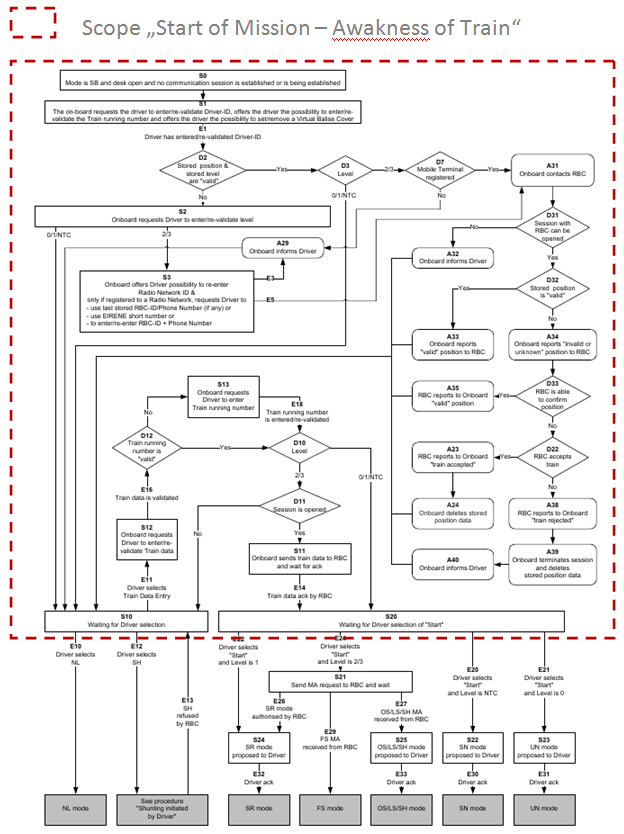
\includegraphics[scale=0.8]{images/SoMAwaknessoftrain}
\caption{Start of Mission - Awakness of Train}
\label{Start of Mission - Awakness of Train}
\end{figure}

\paragraph{Interface}
\textbf{Input Flow}
\begin{itemize}
\item Information from TIU
\item Action from Driver (DMI)
\item Information from Position Calculation
\item Information from Persistent Data
\item Information from Management of Radio Communication
\item Information from Mode and Level Management (Level and Mode Status)
\item Information from Radio Block Control
\end{itemize}

\textbf{Output Flow}
\begin{itemize}
\item Information to Management of Radio Communication
\item Request to Management of Radio Communication
\item Request to Driver (DMI)
\item Request to Mode and Level Management (Request Mode Change)
\item Request to Radio Block Control (Validation of Train Data)
\end{itemize}

\paragraph{Functional Design Description}
For the third iteration just a part of the Scope has been design. To complete the scenario in the third iteration the ideal path to the awakness of train until the state "waiting for Driver selection of "Start"" have been realized. Furthermore the initial data from the persistend database such as Level, Driver ID, Train Number, Train Data, Radio Number, RBC ID hase been consider as constants. 

\paragraph{Refernce to the Scade Model}
\url{https://github.com/openETCS/modeling/blob/master/model/Scade/System/ObuFunctions/Procedures/ManageProcedure_Pkg.xscade}

\subsubsection{Start of Mission in Level 2 or 3 Mode SR FS OS LS SH}
\paragraph{Reference to the SRS or other Requirements (or other requirements)}
Chapter 5, § 5.4
\paragraph{Short description of the functionality}
This functionality describes the Start of Mission procedure of the train in Level 2 or 3 and the Modes SR FS OS LS SH where the train under the defined Mode Level supervision starts running.
See scope of the Start of Mission - Level 2 or 3 and Modes SR FS OS LS SH in the figure below.
\begin{figure}[h]
\centering
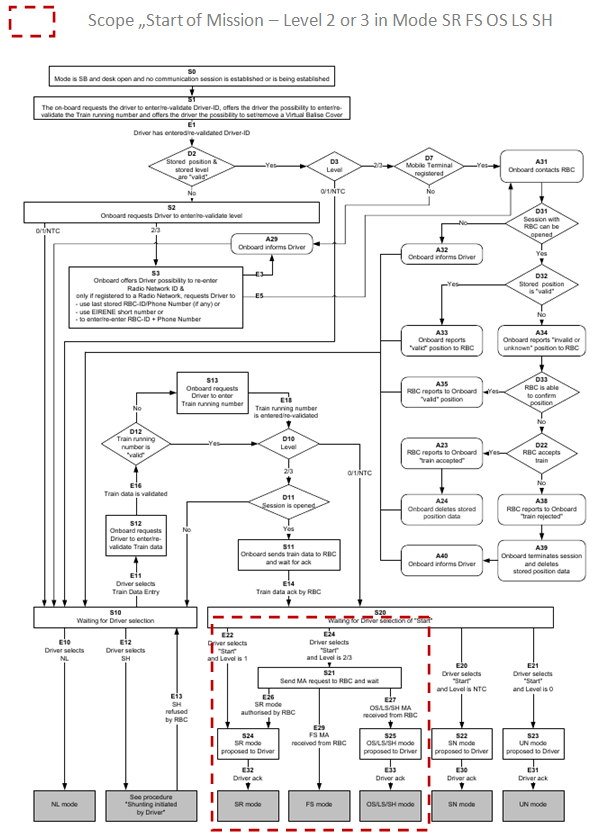
\includegraphics[scale=0.7]{images/SoMLevel2_3_SR_FS_OS_LS_SH}
\caption{Start of Mission - Start of Mission in Level 2 or 3 and Mode SR FS OS LS SH}
\label{Start of Mission - Start of Mission in Level 2 or 3 and Mode SR FS OS LS SH}
\end{figure}

\newpage

\paragraph{Interface}
\textbf{Input Flow}
\begin{itemize}
\item Action from Driver (DMI)
\item Information from Mode and Level Management (Level and Mode Status)
\item Information from Movement Authority Managmement (Receiving of Movement Authority)
\end{itemize}

\textbf{Output Flow}
\begin{itemize}
\item Request to Driver (DMI)
\item Request to Movement Authority Management (Request Movement Authority)
\item Request to Mode and Level Management (Request Mode Change)
\end{itemize}


\paragraph{Functional Design Description}
For the third iteration just a part of the Scope has been design. To complete the scenario in the third iteration the path "Full Supervision Movement Authority received from RBC" has been realized. The state will end after the train receives the Change Authority to FS and will be ready to run.

\paragraph{Refernce to the Scade Model}
\url{https://github.com/openETCS/modeling/blob/master/model/Scade/System/ObuFunctions/Procedures/SoM_SR_FS_OS_LS_SH_SN_UN.xscade}



%-----------------------------------------------------------------------
\subsection{Manage Track Data}
%-----------------------------------------------------------------------
%\tbc
%Jakob Gärtner

\subsubsection{F.2.2 Calculate Train Position}\label{sss:calctrainpos}

\begin{itemize}
\item \textbf{Short Description of Functionality}\\
The main purpose of the function is to calculate the locations of linked and unlinked balise groups (BGs) and the current train position while the train is running along the track. 

\begin{figure}[hbtp]
\centering
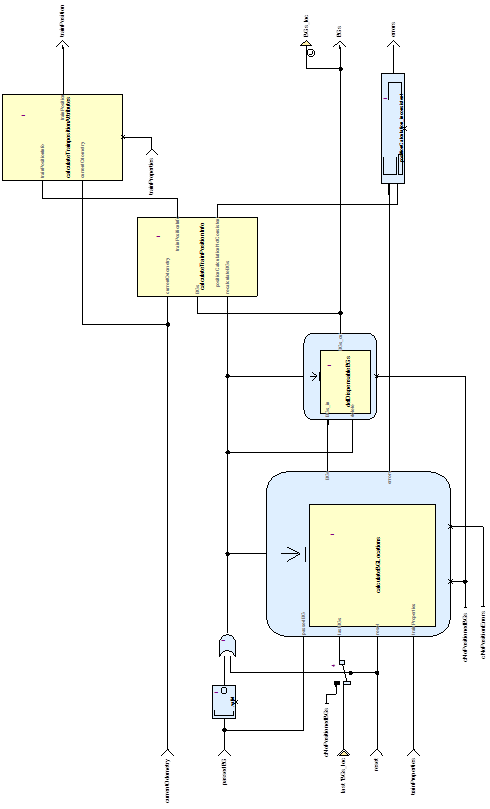
\includegraphics[scale=1]{../images/CalculateTrainPosition.png}
\caption{Structure of calculateTrainPosition}
\end{figure}


\paragraph{Functional Structure in Stages}
The whole function calculateTrainPosition is subdivided into the following steps, which are performed sequentially: 
\begin{enumerate}
\item \textbf{\textit{calculateBGLocations}}: Calculate the balise group locations\\
The first stage is triggered each time the train passes a balise group (input \textit{passedBG}). It takes the balise group header with the BG identification, the linking information (Subset 26, packet 5) and the current odometry values as inputs and calculates the location of the the passed balise group. If the passed BG has been announced via linking information previously, it takes into account the linking as well as the odometry information. If the passed BG does not meet the tolerance window announced by linking, an error flag is set. If the passed BG is an unlinked BG, its location is determined by odometry only, but related to the next previously passed linked BG, if there is one.\\
Then, if the passed BG is a linked BG comprising linking information for BGs ahead, the linking information is evaluated by creating the announced BGs and computing their locations from the linking distances.\\
The passed and the announced BGs are stored in a list \textit{BGs}, ordered by their nominal location on the track.\\
Afterwards the locations of all BGs are further improved by re-adjusting their locations with reference to the just passed BG. This optimizes the BG location inaccuries around the current train position (= location of the passed BG). 

\item \textbf{\textit{delDispensableBGs}}: Delete dispensable balise groups\\
The second stage removes balise groups supposed not to be needed any longer from the list of \textit{BGs}.\\
If the number of stored passed linked BGs exceeds the maximum number of eight as specified in subset-26-3.6.2.2.2 c), all BGs astern are deleted.
If only (passed) unlinked BGs are in the list and exceed the number of \textit{cNoOfAtLeast\_x\_unlinkedBGs}, all passed BGs astern to those are removed from the list. 

\item \textbf{\textit{calculateTrainPositionInfo}}: Calculate train position information.\\
This stage take the list of stored BGs and the current odometry values as inputs and steadily provides the current train position. 

\item \textbf{\textit{calculateTrainpositionAttributes}}: Calculate train position attribute information.\\
This stage provides several additional position related attributes that might conveniently be used by subsequent consumers in the architecture. It requires the actual LRBG and the previous LRBG to be assigned external from the list \textit{BGs}. 

\end{enumerate}

\item \textbf{Reference to the SRS (or other requirements)}\\
\\
The component calculateTrainPosition determines the location of linked and unlinked balise groups and the current train position during the train trip as specified mainly in subset-026-3.6

\item \textbf{Design Constraints and Choices}\\
\\
The following constraints and prerequisites apply:

\begin{enumerate}
\item The input data received from the balises groups must have been checked and filtered for validity, consistency and the appropriate train orientation before delivering them to calculateTrainPosition. 
\item The storage capacity for balise groups is finite. calculateTrainPosition will raise an error flag when a balise group cannot be stored due to capacity limitations.
\item calculateTrainPosition will raise an error flag if a just passed balise group is not found where announced by linking information. It will not (yet) detect when an announced balise group is missing. 
\item calculateTrainPosition is not yet prepared for train movement direction changes. 
\item calculateTrainPosition does not yet consider repositioning information.
\end{enumerate}

\end{itemize}

\subsubsection{Provide Position Report}\label{sss:provposrep}

\begin{figure}[ht]
\centering
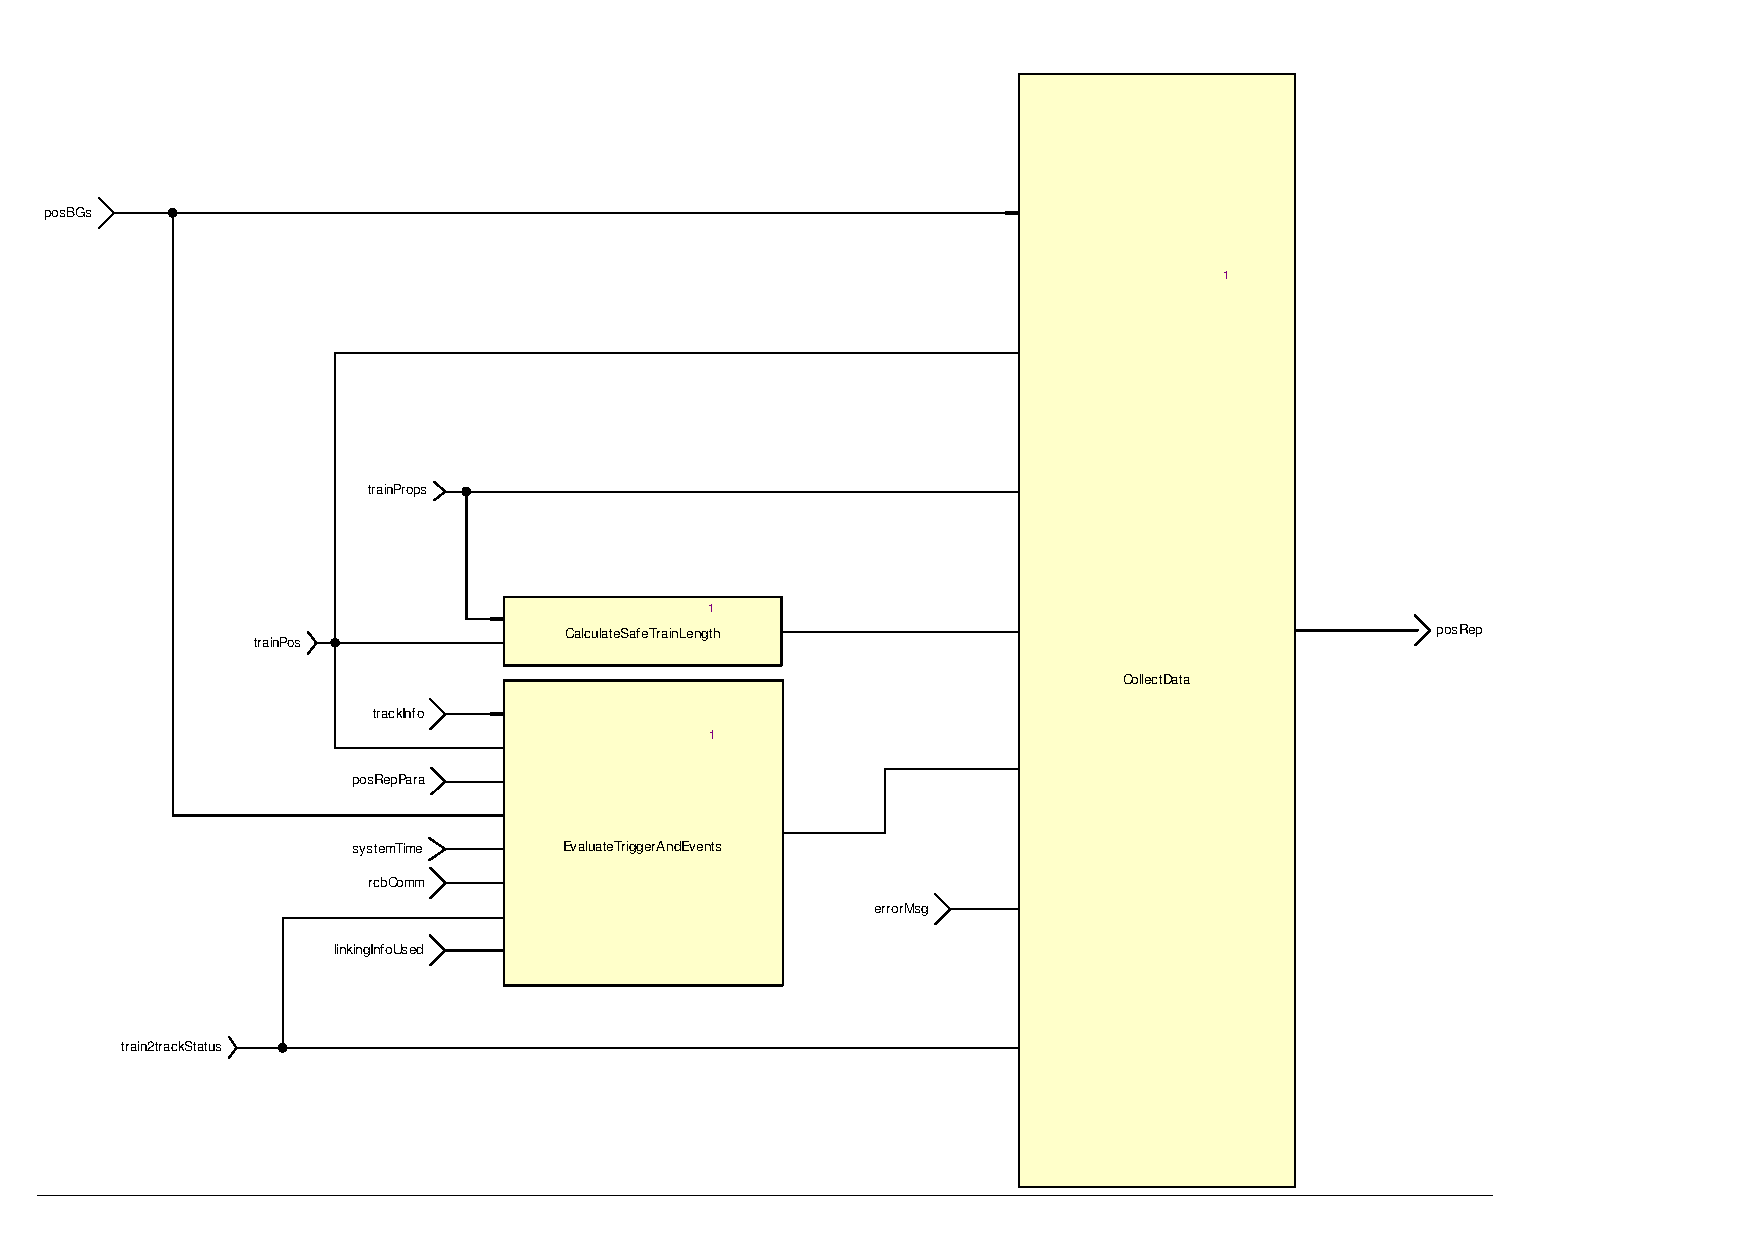
\includegraphics[scale=0.6]{../images/ProvidePositionReport.pdf}
\caption{Structure of component ProvidePositionReport}\label{fig:provideposrep}
\end{figure}

\begin{itemize}
\item \textbf{Short Description of Functionality}\\
This function takes the current train position and generates a position report which is sent to the RBC. The point in time when such a report is sent is determined from event, on the one hand, and position report parameters---which are basically triggers---provided by the RBC or a balise group passed, on the other hand. The functionality is modeled using three operations, as shown in Fig.~\ref{fig:provideposrep}, which are explained below.
\begin{description}
	\item[CalculateSafeTrainLength] Calculates the the safeTrainLength according to Chapt.~3.6.5.2.4/5.
\verb+safeTrainLength = absolute(EstimatedFrontEndPosition - MinSafeRearEnd)+, where
\verb+MinSafeRearEnd = minSafeFrontEndPosition - L_TRAIN+
	\item[EvaluateTriggerAndEvents] Returns a Boolean modeling whether the sending of the next position report is triggered or not. It is the conjunction of the evaluation of all triggers (PositionReportParameters, i.e., Packet 58) and events (see Chapt.~3.6.5.1.4).
	\item[CollectData] In this operation, data of Packet0, \dots, Packet5 and the header is aggregated to a position report.
\end{description}
\item \textbf{Reference to the SRS (or other requirements}\\
Most of the functionality is described in subset 26, chapter~3.6.5.
\item \textbf{Design Constrains and Choices}\\
\begin{enumerate}
	\item The message length (i.e., attribute \verb+L_MESSAGE+) is by default set to 0; the actual value will be set by the Bitwalker/API.
	\item The attribute \verb+Q_SCALE+ is assumed to be constant; that is, all operations using this attribute do not convert between different values of that attribute.
	\item \textit{PositionReportHeader}: The time stamp (i.e., attribute \verb+T_TRAIN+) is not set; this should be done once the message is being sent by the API
	\item \textit{Packet4}: When aggregating the data for this packet, an error message might be overwritten by a succeeding error message. Because the specification only allows to sent one error in one position report, errors are not being stored in a queue, for instance.
	\item \textit{Packet44}: This packet is currently not contained in a position report as it is not part of the kernel functions.
	\item The usage of attributes \verb+D_CYCLOC+ and \verb+T_CYCLOC+ as part of the triggers specified by the position report parameters (i.e., Packet 58 sent by the RBC) may lead to unexpected results if a big clock cycle together with small values for the attributes is used. The cause is that the current model increments at every clock cycle the reference value for the distance and time by at most \verb+D_CYCLOC+ and \verb+T_CYCLOC+, respectively and not a factor of it.
\end{enumerate}
\item \textbf{Open Issues}
\begin{enumerate}
	\item Operation \textit{EvaluateTriggerAndEvents} currently ignores parameters \verb+N_ITER+, \verb+D_LOC+ and \verb+D_LGTLOC+ which allow to specify up to 32 position at which a report has to be sent. The positions are relative to the location of a reference balise group. If the RBC sends packet 58, then it also provides a reference balise group; otherwise, if packet 58 is sent by a balise group, then this balise group serves a the reference balise group. Possible realisation in the model: Extend in the interface posRepPara (i.e., Packet 58) by a \verb+NID_BG+ referring to the reference balise group. Am assumption would be that this BG can be found in the list of passed balise group provided by \textit{CalculateTrainPosition} in Sect.~\ref{sss:calctrainpos}.
	\item The specification requires to store the last eight balise groups for which a position report has been sent (see 3.6.2.2.2.c).
	\item For all reports that contain Packet 1 (i.e., report based on two balise groups), the RBC sends a coordinate system. It is unclear where this has to be stored (i.e., somehow the balise groups have to be stored in a database which has then to be updated), see 3.4.2.3.3.6. Moreover, such a coordination system can be invalid and then has to be rejected (see 3.4.2.3.3.7-8). On a more abstract level, we need to think about the interface between the RBC and the OBU or a proper abstraction thereof.
	\item The decision whether a the report consists of packet 0 or packet 1, which is provided in 3.4.2.3.3, is currently not completely modeled. So far, 3.4.2.3.3.1 has only been modeled, thereby assuming ``the last balise group detected'' is the last balise group and not the LRBG. 3.4.2.3.3.2 is unclear. To model 3.4.2.3.3.4 I need information about the last two valid balise groups and the train running direction. This information can be obtained by adding a memory or this information will be provided by \textit{CalculateTrainPosition} in Sect.~\ref{sss:calctrainpos}. Likewise, also 3.4.2.3.3.5 requires knowledge about the last two valid balise groups.
\end{enumerate}
\end{itemize}
 


%\subsubsection{functional block x in Manage Track Data}%MainfunctionManage Track Data.. Name should be be defined and substituded by the designer of the function. 
%\paragraph{Reference to the SRS or other Requirements (or other requirements)}
%\paragraph{Short descriptoiin of the functionality}
%\paragraph{Interface}
%\paragraph{Functional Design Description}
%\paragraph{Refernce to the Scade Model}
%\textbf{only in special case or link to the Scade model}

%\subsubsection{functional block x in Manage Track Data}%Mainfunction Manage Track Data. Name should be be defined and substituded by the designer of the function. 
%\paragraph{Reference to the SRS or other Requirements (or other requirements)}
%\paragraph{Short descriptoiin of the functionality}
%\paragraph{Interface}
%\paragraph{Functional Design Description}
%\paragraph{Refernce to the Scade Model}
%\textbf{only in special case or link to the Scade model}

%\subsubsection{functional block x in Manage Track Data}%Mainfunction Manage Track Data. Name should be be defined and substituded by the designer of the function. 
%\paragraph{Reference to the SRS or other Requirements (or other requirements)}
%\paragraph{Short descriptoiin of the functionality}
%\paragraph{Interface}
%\paragraph{Functional Design Description}
%\paragraph{Refernce to the Scade Model}
%\textbf{only in special case or link to the Scade model}

%\subsubsection{functional block x in Manage Track Data}%Mainfunction Manage Track Data. Name should be be defined and substituded by the designer of the function. 
%\paragraph{Reference to the SRS or other Requirements (or other requirements)}
%\paragraph{Short descriptoiin of the functionality}
%\paragraph{Interface}
%\paragraph{Functional Design Description}
%\paragraph{Refernce to the Scade Model}
%\textbf{only in special case or link to the Scade model} 



%-----------------------------------------------------------------------
\subsection{Mode and Level}
%-----------------------------------------------------------------------
%\tbc
%Marielle Petit


The "Management of Modes and Levels" function is mainly described in chapter 4
and 5 of \citep{subset-026}. Modes and levels define the status of the ETCS
regarding on-board functional status and track infrastructure.

\begin{landscape}
\begin{figure}[hbtp]
\centering
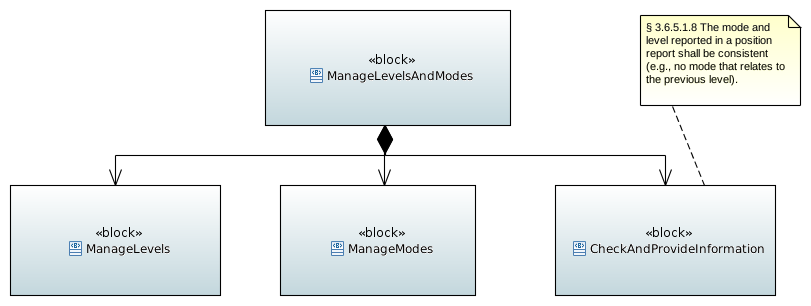
\includegraphics[scale=1]{images/FunctionalArchitecture.png}
\caption{High level Architecture}
\end{figure}
\end{landscape}

\subsubsection{Function Level Management}%Mainfunction receive track data. Name should be be defined and substituded by the designer of the function.
\paragraph{Reference to the SRS or other Requirements}

see \citep{subset-026} section 5.10

\paragraph{Short description of the functionality}

The level management subsystem receives level transition order tables and selects the order with the highest probability. It stores the information about the selected transition order and transits to the requested level once the train passes the location of the level transition.

If required, the driver is asked to acknowledge the transition, in case of no acknowledge or if conditions for the level transition are not fulfilled, the train gets tripped.

\paragraph{Interface}

The interface consists of the following inputs:

\begin{itemize}
\item \emph{conditional transitions:} a priority table containing the
  conditional level transition orders (from paquet 46)
\item \emph{level transition priority table:} a priority table containing the
  (non-conditional) level transition orders (from paquet 41)
\item \emph{train standstill:} a Boolean value indicating whether the train is
  at standstill (from odometry)
\item \emph{driver level transition:} a level transition order selected by the
  driver (from DMI)
\item \emph{ERTMS capabilities:} the ERTMS capabilities of the track
\item \emph{getAck:} Boolean input that signals the acknowledgment of the
  driver (from DMI)
\item \emph{resetIdle:} Boolean input to reset without acknowledge
\item \emph{currentDistance:} the current position of the train given with the
  same reference as the position of the level transition order (train position , from localisation)
\item \emph{ackDistance:} the maximal distance for driver acknowledge after
  the level transition (from paquet 41)
\item \emph{immediateAck:} a Boolean that signals that an immediate acknowledge
  is required
\item \emph{received L2 L3 MA:} a Boolean that indicates that a level 2 or level
  3 movement authority for the track behind the level transition has been
  received (from paquet 15)
\item \emph{received L1 MA:} a Boolean that indicates that a level 1 movement
  authority for the track behind the level transition has been received (from paquet 12)
\item \emph{received target speed:} a Boolean indicating that a target speed for
  the track behind the level transition has been received (from paquet 27) ?
\end{itemize}

and the following outputs:

\begin{itemize}
\item \emph{next level:} the next level after this computation cycle
\item \emph{Trip train:} a Boolean indicating whether the train should be
  tripped
\item \emph{previous level:} the previous level before this computation cycle
\item \emph{needsAckFromDriver:} a Boolean that indicates whether an
  acknowledgment from the driver is necessary
\end{itemize}

\paragraph{Functional Design Description}

On the most abstract level the design consists of the \emph{manage\_priorities} function which takes the level transition order priority tables as inputs and computes the highest priority transition.

This transition order is the fed to the \emph{computeLevelTransitions} operator. This operator consists of three main parts. The \emph{ComputeTransitionConditions} operator that emits the fulfilled conditions to change from a given level to a new level, the \emph{LevelStateMachine} that stores the current level and takes the computed change conditions as input for possible level transitions and finally the \emph{driverAck} operator which contains a state machine that stores the information whether the system is currently waiting for a driver acknowledge and emits the train trip information if necessary.


\paragraph{Reference to the Scade Model}

The Scade model is available on github:
\url{https://github.com/openETCS/modeling/tree/master/openETCS ArchitectureAndDesign/Work Groups/Group 3/SCADE/LevelManagement/}

%%%%%%%%%%%%%%%%%%%%%%%%%%%%%%%%%%%%%%%%%%%%%%%%%%%%

\subsubsection{Function Mode Management}%Mainfunction receive track data. Name should be be defined and substituded by the designer of the function.
\paragraph{Reference to the SRS or other Requirements}
see \citep{subset-026} sections 4.4, 4.6, 5.4, 5.5, 5.6, 5.7, 5.8, 5.9, 5.11, 5.12, 5.13, 5.19

\paragraph{Short description of the functionality}


This function is in charge of the computation of new mode to apply according to conditions from inputs (track information, driver interactions, train data,...) and other functions.

\paragraph{Interface}

The inputs are the following:
\begin{itemize}
\item \emph{Cab} identification of the current cabin (A or B)
\item \emph{Continue\_shunting\_Function\_Active}: boolean to describe the activation state of the shunting function
\item \emph{Current\_Level}: outputs of the Level management function
\item \emph{Data\_From\_DMI}: set of data received from the driver via the DMI interface, indeed:
\begin{itemize}
\item \emph{Ack\_LS : bool} Driver acknoledges LS mode
\item \emph{Ack\_OS : bool}
\item \emph{Ack\_RV : bool}
\item \emph{Ack\_SH : bool}
\item \emph{Ack\_SN : bool}
\item \emph{Ack\_SR : bool}
\item \emph{Ack\_TR : bool}
\item \emph{Ack\_UN : bool}
\item \emph{Req\_Exit\_SH : bool} driver selects exit of shunting
\item \emph{Req\_NL : bool} Driver requests NL mode
\item \emph{Req\_Override : bool} Driver requests override function
\item \emph{Req\_SH : bool} driver requests SH mode
\item \emph{Req\_Start : bool} Driver requests start of mission
\item \emph{ETCS\_Isolated: bool}: isolation status of the ETCS
\end{itemize}
\item \emph{Data\_From\_Localisstion}: set of data received from the function in charge of localistion of the train, indeed:
\begin{itemize}
\item \emph{BG\_In\_List\_Expected\_BG\_In\_SR : bool}: the identity of the overpass balise group is in the list of expected balises related to SR mode (from SR to trip mode condition 36)
\item \emph{BG\_In\_List\_Expected\_BG\_In\_SH : bool}: the identity of the overpass balise group is in the list of expected balises related to SH mode (from SH to trip mode condition 52)
\item \emph{Linked\_BG\_In\_Wrong\_Direction : bool} balise group contained in the linking information is passed in the unexpected direction (from FS, LS, OS to trip mode condition 66) \emph{Localisaion function ?}
\item \emph{Train\_Position}: output provided by function in charge of computation of train possition (type	TrainPosition\_Types\_Pck::trainPosition\_T)	\item \emph{Train\_Speed : Obu\_BasicTypes\_Pkg::Speed\_T} provided by odometry function
\item \emph{Train\_Standstill : bool} provided by odometry function
\end{itemize}
\item \emph{Data\_From\_Speed\_and\_Supervision}: set of data received from the function in charge of speed and supervision management, indeed:
\begin{itemize}
\item \emph{Estim\_front\_End\_overpass\_SR\_Dist : bool}: the train overpass the SR distance with its estimated front end (from SR to trip mode condition 42) 
\item \emph{Estim\_Front\_End\_Rear\_SSP : bool}: estimated front end is rear of the start location of either SSP or gradient profile stored on-board (from FS, LS, OS to trip mode condition 69)
\item \emph{Override\_Function\_Active}: boolean to indicate the state of the activation function 	  	
\item \emph{EOA\_Antenna\_Overpass : bool}: the train overpasses the  EOA  with min safe antenna position Level 1 (from FS, LS, OS to trip mode condition 12)
\item \emph{EOA\_Front\_End : bool} the train overpasses the  EOA  with min safe front end, Level 2 or 3 (from FS, LS, OS to trip mode condition 16)
\item \emph{Train\_Speed\_Under\_Overide\_Limit : bool} supervision when override function is active (to SR mode condition 37)
\end{itemize}
\item \emph{Data\_From\_TIU : TIU\_Types\_Pkg::Message\_Train\_Interface\_to\_EVC\_T}:message provided by TIU interface
\item \emph{Data\_From\_Track}: set of data received from track side (via RBC or Balises telegram), indeed:
\begin{itemize}
\item \emph{MA\_SSP\_Gradiant\_Available : bool} MA, SSP and gradient have been received, checked and stored on-board from paquet 12, 15, 21 and 27 or message 3 or 33
\item \emph{Mode\_Profile\_On\_Board : Level\_And\_Mode\_Types\_Pkg::T\_Mode\_Profile} from packet 80
\item \emph{Shunting\_granted\_By\_RBC : bool} from message 27 and 28
\item \emph{Trip\_Order\_Given\_By\_Balise : bool}
\item \emph{List\_Bg\_Related\_To\_SR\_Empty : bool} from packet 63
\item \emph{Stop\_If\_In\_shunting : bool} from packet 135
\item \emph{Stop\_If\_In\_SR : bool} from packet 137
\item \emph{Error\_BG\_System\_Version : bool}
\item \emph{Linking\_Reaction\_To\_Trip : bool}
\item \emph{RBC\_Ack\_TR\_EB\_Revocked : bool} from message 6
\item \emph{RBC\_Authorized\_SR : bool} from message 2
\item \emph{Reversing\_Data : Level\_And\_Mode\_Types\_Pkg::T\_Reversing\_Data} from packet 138/ 139
\item \emph{T\_NVCONTACT\_Overpass : bool} Maximal time without new safe message overpass
\item \emph{Emergency\_Stop\_Message\_Received}: boolean to describe the reception of Emergency Stop message  from message 15 or 16
\end{itemize}
\item \emph{Failure\_Occured}: boolean to indicate safety failure occurence	
\item \emph{Interface\_To\_National\_System}: boolean to indicate existance of an interface to a national system 	  	
\item \emph{National\_Trip\_Order}: boolean to indicate reception of a trip order from a national system 	  	
\item \emph{OnBoard\_Powered}: boolean to indicate the poxering state of the system 	  	
\item \emph{Stop\_Shunting\_Stored}: boolean to store the information in regards of shunting function	  	
\item \emph{Valid\_Train\_Data\_Stored}: boolean to indication train data are available and valid.
\end{itemize}

The outputs are the following:

\begin{itemize}
\item \emph{currentMode} the new computed mode (typeis  Level\_And\_Mode\_Types\_Pkg::T\_Mode, default value is Level\_And\_Mode\_Types\_Pkg::SB )
\item \emph{EB\_Requested} boolean to request triggering of emergency brake 	  	
\item \emph{Service\_Brake\_Command} boolean to request command of service brake 	  	
\item \emph{Data\_To\_DMI}: set of data provided to the DMI	Level\_And\_Mode\_Types\_Pkg::T\_Data\_To\_DMI 	:  	
\begin{itemize}
\item \emph{Ack\_LS : bool} Driver acknoledges LS mode
\item \emph{Ack\_OS : bool}
\item \emph{Ack\_RV : bool}
\item \emph{Ack\_SH : bool}
\item \emph{Ack\_SN : bool}
\item \emph{Ack\_SR : bool}
\item \emph{Ack\_TR : bool}
\item \emph{Ack\_UN : bool}
\item \emph{Req\_Exit\_SH : bool} driver selects exit of shunting
\item \emph{Req\_NL : bool} Driver requests NL mode
\item \emph{Req\_Override : bool} Driver requests override function
\item \emph{Req\_SH : bool} driver requests SH mode
\item \emph{Req\_Start : bool} Driver requests start of mission
\item \emph{ETCS\_Isolated: bool}: isolation status of the ETCS
\end{itemize}
\item \emph{Data\_To\_BG\_Management}: set of date to trackside Level\_And\_Mode\_Types\_Pkg::T\_Data\_To\_BG\_Management 	: 
\begin{itemize}
\item \emph{EoM\_Procedure\_req : bool} request of end of mission procedure indeed end of the communication session for message 150
\item \emph{Clean\_BG\_List\_SH\_Area : bool} request to clean the BG  list when entering  an SH area §5.6.2
\item \emph{MA\_Req : bool} for message 132
\item \emph{Req\_for\_SH\_from\_driver : bool} for message 130
\end{itemize}
\end{itemize}

\paragraph{Functional Design Description}


Three subfunctions are defined:
\begin{description}
\item[Inputs] proceeds to inputs check and preparation.
\item[ComputeModesCondition] performs all specific procedure linked to mode management and defined in  \citep{subset-026} sections 5.4, 5.5, 5.6, 5.7, 5.8, 5.9, 5.11, 5.12, 5.13, 5.19 and specifies the conditions to define a mode transition according condition table of section 4.6.3 of \citep{subset-026}
\item[SwitchModes] performs the mode selection according the conditions and priorities defined in transition table  section 4.6.2 of \citep{subset-026}
\item[Outputs] prepares paquet of outputs.
\end{description}


\begin{landscape}
\begin{figure}[hbtp]
\centering
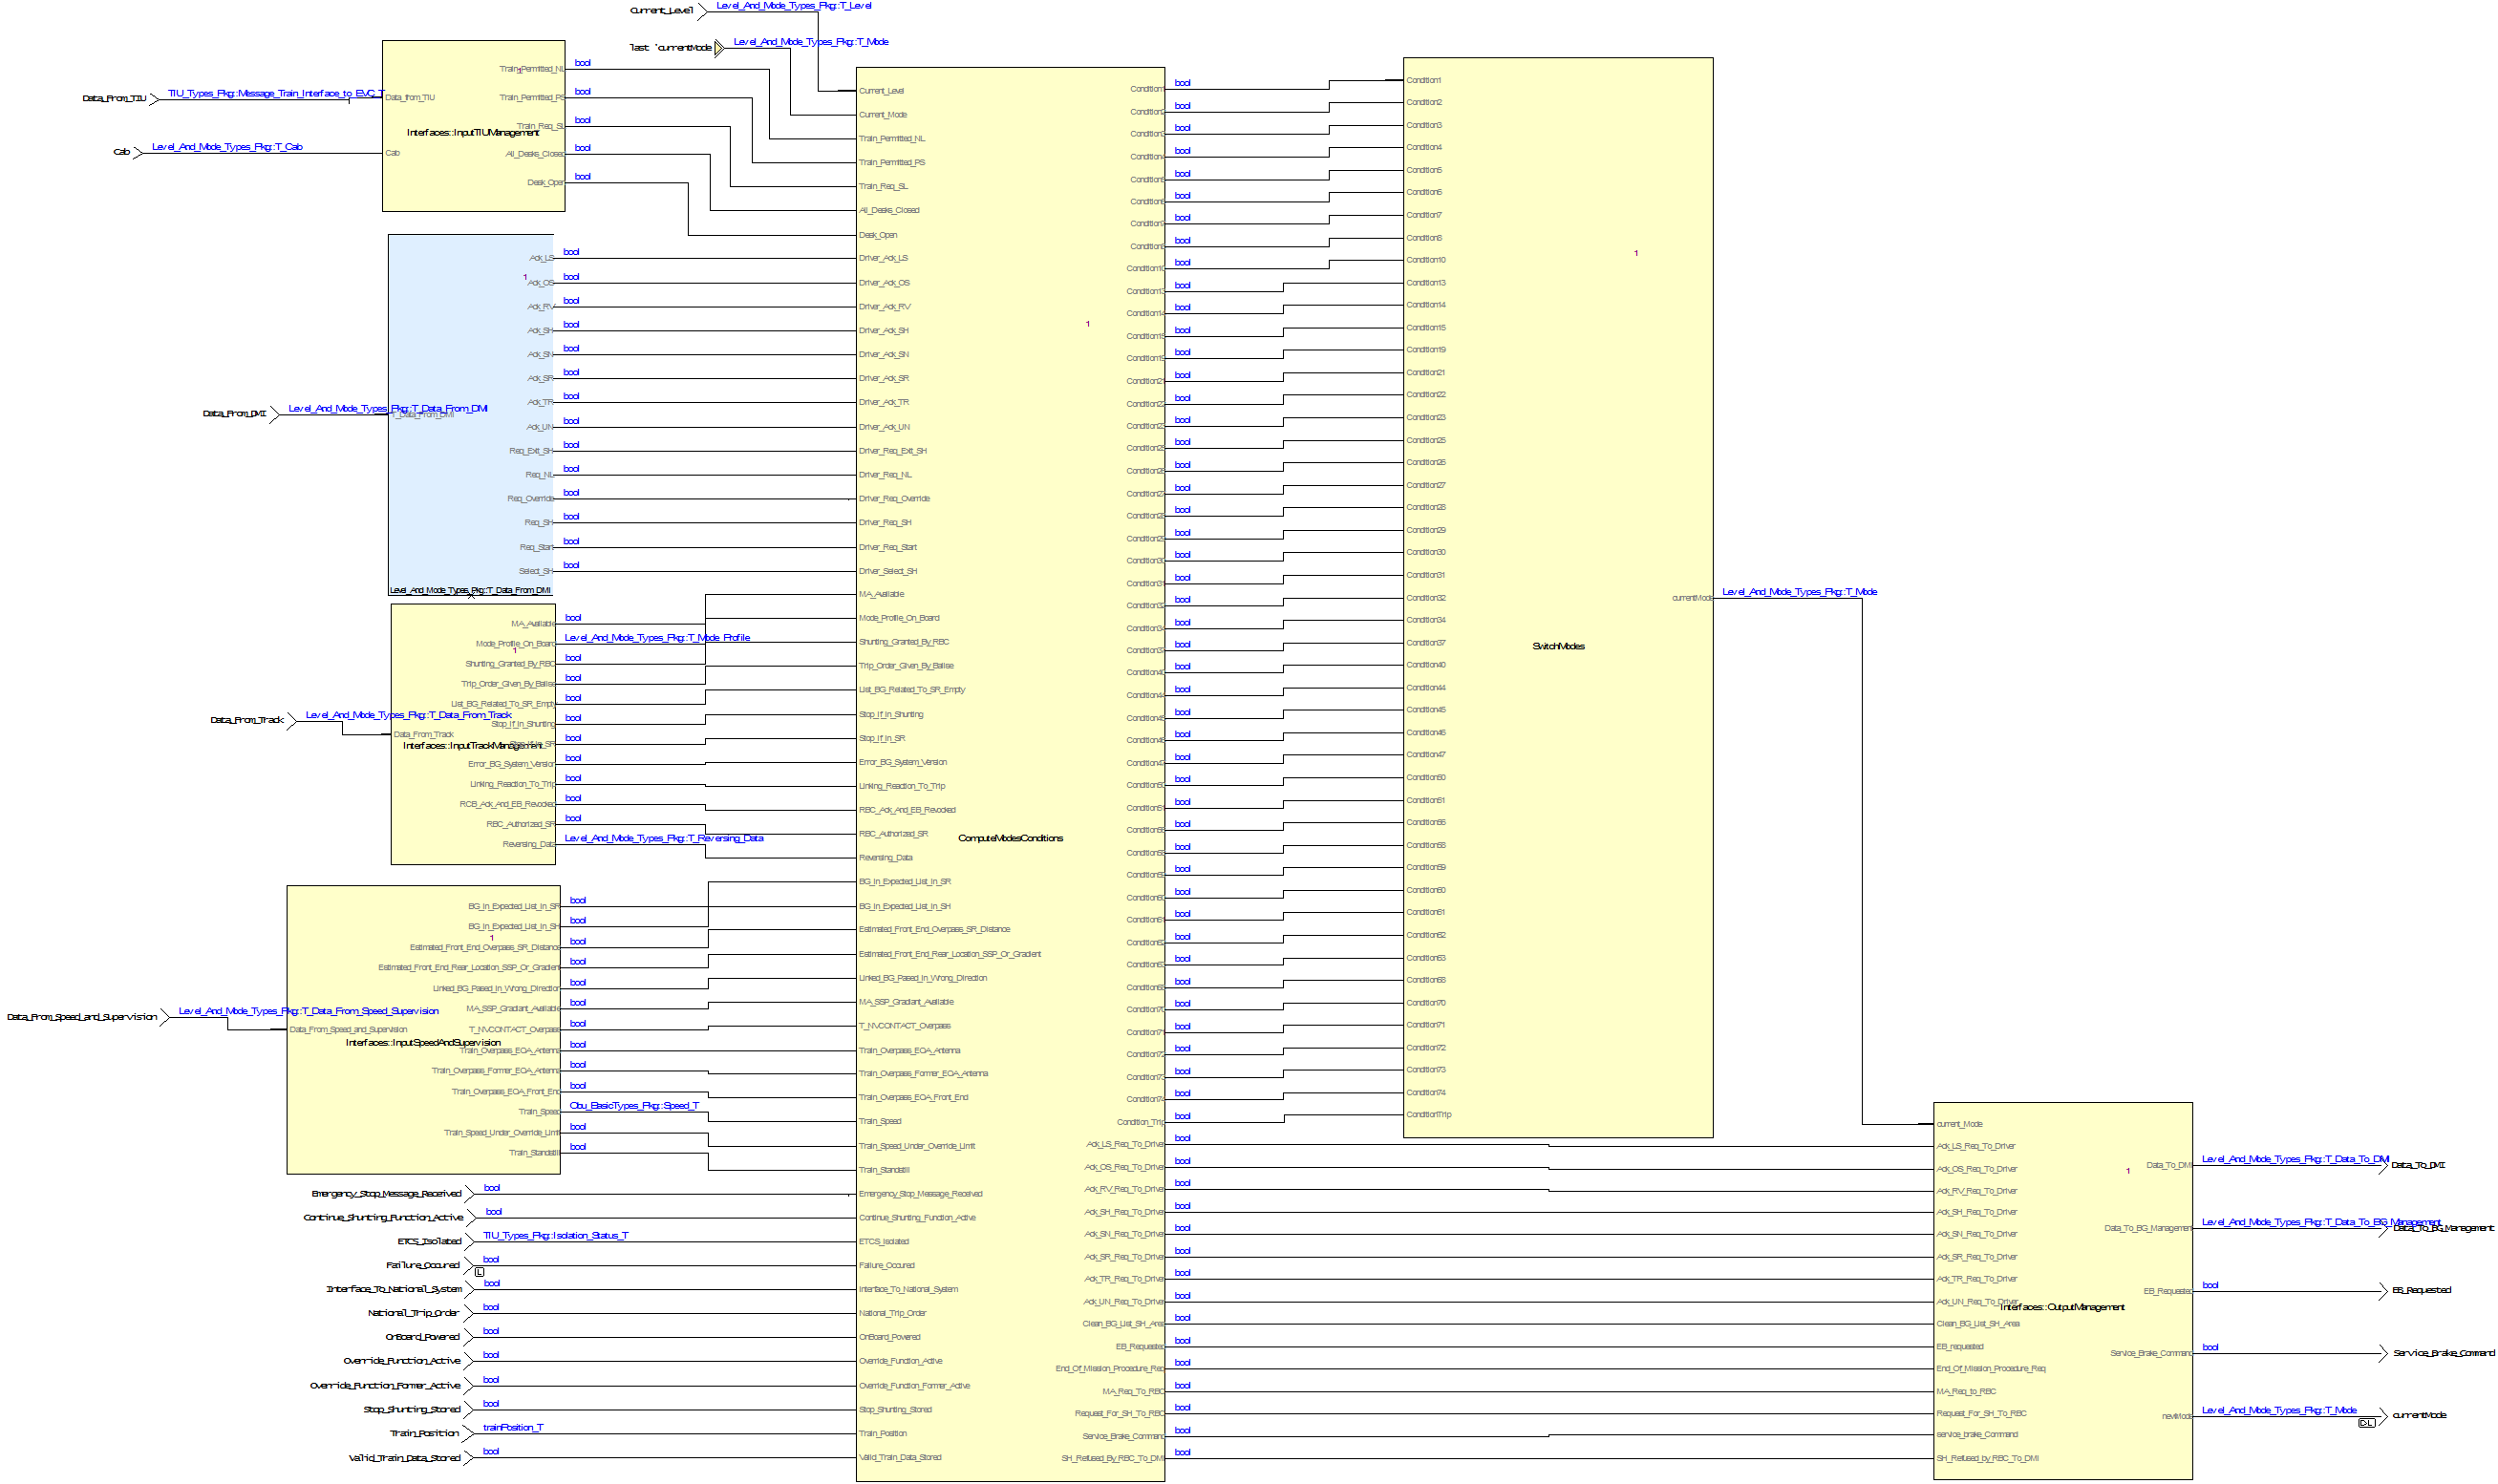
\includegraphics[scale=0.3]{images/ManageModes.png}
\caption{Modes subfubction architecture}
\end{figure}
\end{landscape}

\paragraph{Reference to the Scade Model}
The Scade model is available on github:
\url{https://github.com/openETCS/modeling/tree/master/model/Scade/System/ObuFunctions/ManageLevelsAndModes/Modes}

%%%%%%%%%%%%%%%%%%%%%%%%%%%%%%%%%%%%%%%%%%%%%%%%%%%%


\subsubsection{Function Check and Provide Level and Mode}%Mainfunction receive track data. Name should be be defined and substituded by the designer of the function.
\paragraph{Reference to the SRS or other Requirements}
see \citep{subset-026} section 3.6.5

\paragraph{Short description of the functionality}
checks compatibility between mode and level and provides outputs

\paragraph{Interface}
\emph{To design}

\paragraph{Functional Design Description}
\emph{To design}

\paragraph{Reference to the Scade Model}
\emph{To design}


%-----------------------------------------------------------------------
\subsection{Manage RBC Procedure}
%-----------------------------------------------------------------------
%\tbc
%Uwe Steinke

\subsubsection{functional block x in Manage RBC Procedure}%Mainfunction receive track data. Name should be be defined and substituded by the designer of the function. 
\paragraph{Reference to the SRS or other Requirements (or other requirements)}
\paragraph{Short descriptoiin of the functionality}
\paragraph{Interface}
\paragraph{Functional Design Description}
\paragraph{Refernce to the Scade Model}
\textbf{only in special case or link to the Scade model}

\subsubsection{functional block x in Manage RBC Procedure}%Mainfunction receive track data. Name should be be defined and substituded by the designer of the function. 
\paragraph{Reference to the SRS or other Requirements (or other requirements)}
\paragraph{Short descriptoiin of the functionality}
\paragraph{Interface}
\paragraph{Functional Design Description}
\paragraph{Refernce to the Scade Model}
\textbf{only in special case or link to the Scade model}

\subsubsection{functional block x in Manage RBC Procedure}%Mainfunction receive track data. Name should be be defined and substituded by the designer of the function. 
\paragraph{Reference to the SRS or other Requirements (or other requirements)}
\paragraph{Short descriptoiin of the functionality}
\paragraph{Interface}
\paragraph{Functional Design Description}
\paragraph{Refernce to the Scade Model}
\textbf{only in special case or link to the Scade model}

\subsubsection{functional block x in Manage RBC Procedure}%Mainfunction receive track data. Name should be be defined and substituded by the designer of the function. 
\paragraph{Reference to the SRS or other Requirements (or other requirements)}
\paragraph{Short descriptoiin of the functionality}
\paragraph{Interface}
\paragraph{Functional Design Description}
\paragraph{Refernce to the Scade Model}
\textbf{only in special case or link to the Scade model}




\chapter{F3: Measure Train Movement}

\chapter{F4: Manage Radio Communication}
%set the master document for easy compilation
%!TEX root = ../D3_5_2.tex


 

\chapter{F5: Manage JRU}

\chapter{F6: DMI Controller}
%set the master document for easy compilation
%!TEX root = ../D3_5_2.tex

  %-----------------------------------------------------------------------
  \subsection{DMI Controller}
  %-----------------------------------------------------------------------
  %\tbc
  %Valerio D´Angelo/Baseliyos Jacob

  \paragraph{Reference to the SRS or other Requirements (or other requirements)}

   ERA\_ERTMS\_015560

  \paragraph{Short description of the functionality}
  The DMI controller interact with the DMI display and is responsible for alls procedures between the DMI display and Driver. Furthermore, the DMI controller will interact with the DMI Management to compute the received information (e.g. driver number request, ...) and send, if necessary, data or reports to the DMI Management (acknowledge, text messages...). The DMI Controller is a passive module, this means that all the processing are performed EVC-side, therefore the DMI Controller simply responds to the requests of the EVC or Driver and performs some checks according with the information received from EVC.

  \begin{figure}
  \centering
  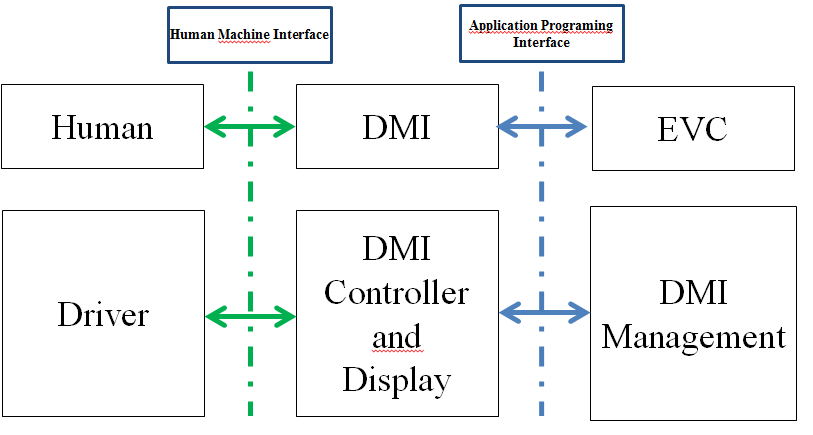
\includegraphics[width=.8\textwidth]{images/DMI_Interfaces}
  \caption{DMI Interfaces}
  \end{figure}

  \paragraph{Interface}
  The DMI Controller has two interfaces. One between DMI Controller and DMI Display and one between DMI Controller and DMI Management. 
  The structure of the interface between DMI Controller and DMI Display is driven by the logic of SCADE Display therefore It doesn't follow any standard or constraints (It will not be described in this chapter).
  DMI Controller and DMI Management exchange packets. Each packet is a structured type with a valid flag (a boolean variable), the DMI controller takes into account the data inside the packet only when the valid flag is true.

  The interface between DMI Controller and DMI Management consist of three parts according with the direction of the information:
  
  \begin{itemize}
  \item From DMI Management to DMI Controller
  \item From DMI Controller to DMI Management 
  \item Both ways directions (You will find the same type both as input than as output)
  \end{itemize}
  


\subparagraph{From DMI Management to DMI Controller}

In the following table are listed the inputs coming from DMI Management with a brief description:\\
  %\begin{table}[H]
    \begin{tabular}{| c | l | l | l | l |}
      \hline
      \textbf{NAME} & \textbf{DESCRIPTION} \\ \hline
      \texttt{DMI\_entry\_request} & Request to input data (e.g. driver id, Train running number etc.)\\
      \texttt{DMI\_identifier\_request} & Request of the DMI informations\\
      \texttt{DMI\_menu\_request} & Request to enable or disable buttons\\
      \texttt{DMI\_dynamic} & Contains informations about current speed, current mode etc.\\
      \texttt{DMI\_text\_message} & Contains predefined or plain text messages\\
      \texttt{DMI\_icons} & Request to display one or more icons in any area\\

      \hline
    \end{tabular} 
  % \caption{Overview of input}
    \label{tbl:DMICtrToDMIMng}
  %\end{table}
  
      Please note: TIU\_trainStatus input is missing in the above table. This is the only input coming directly from TIU and contains the open/close Desk signal. 
    
  \subparagraph{From DMI Controller to DMI Management}
  In the following table are listed the outputs directed to DMI Management with a brief description:\\
  %\begin{table}[H]
    \begin{tabular}{| c | l | l | l | l |}
      \hline
      \textbf{NAME} & \textbf{DESCRIPTION} \\ \hline
      \texttt{DMI\_identifier} & Information about DMI (e.g. version, cabin identifier etc.)\\
      \texttt{DMI\_driver\_request} & Driver request or acknowledgement\\
      \texttt{DMI\_train\_data\_ack} & Train data acknowledgement\\
      \texttt{DMI\_status\_report} & The actual status of DMI (keep alive)\\
      \texttt{DMI\_text\_message\_ack} & Text message acknowledgement\\
      \texttt{DMI\_icons\_ack} & Icon acknowledgement\\

      \hline
    \end{tabular} 
  % \caption{Overview of input}
    \label{tbl:DMICtrToDMIMng}
  %\end{table}
    
\subparagraph{Both ways direction}
In the following table are listed the outputs/inputs  to/from DMI Management with a brief description:\\
  
  %\begin{table}[H]
    \begin{tabular}{| c | l | l | l | l |}
      \hline
      \textbf{NAME} & \textbf{DESCRIPTION} \\ \hline
      \texttt{DMI\_driver\_identifier} & Contains the default or entered driver identifier\\
      \texttt{DMI\_train\_running\_number} & Contains the default or entered train running number\\
      \texttt{DMI\_train\_data} & Contains the default or entered train data\\
      \hline
    \end{tabular} 
  % \caption{Overview of input}
    \label{tbl:DMICtrToDMIMng}
  %\end{table}
  

\paragraph{Functional Design Description}
  \textbf{Please note}: \textit{DMI Controller is a project under construction, a lot of features and functionalities are missing, therefore the structure described below is a draft version and will be changing in the future.}
  
  The informations (received and sent) could be divided in two groups: Sporadic and Periodic. The first one are received/sent aperiodically in any time instead the second one are received/sent periodically, with a fixed deadline. Are part of Periodic group the output DM\_status\_report and the input DMI\_dynamic all other are Sporadic. Therefore, the structure of DMI Controller module consists of a first main state machine \textit{CabinSM} (Fig. \ref{fig:CabinSM}) triggered by  a \textit{OpenDesk} signal (from TIU). Inside the \textit{DeskIsOpen} state there are other two state machines :\textit{HandshakeSM} and \textit{DynamicInfoSM} (Fig. \ref{fig:DynSporSM}).
  
  HandshakeSM performs an initial handshake between DMI Controller and DMI Management. Before that, no data has to be sent or received to/from DMI Management. When the transition is fired a DMI\_identifier packet is sent to DMI Management with informations about the DMI (e.g. DMI identifier, DMI name etc.). At this point the DMI Controler is ready to manage the sporadic information (e.g. Enter or revalidate DriverID, Enter or revalidate Train running number etc.). 
  
  The DynamicInfoSM state machine is triggered after the handshake, exactly when  HandshakeSM reaches the  DynInfo\_Activated state. At the time when the transition is fired a signal is emitted (startDMI\_status) and begins a periodic sending of DMI status information (keep alive) to DMI Management. Once reached DynamicInfo\_Active, the DMI Controller is ready to receive and manage the dynamic informations.
  
   \begin{figure} 
      	\centering
      	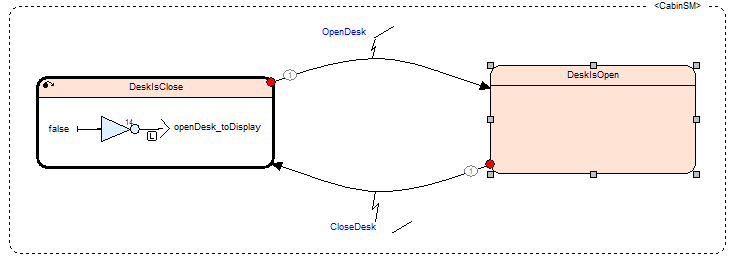
\includegraphics[scale=0.7]{images/CabinSM}
      	\caption{Cabin State Machine.}
      	\label{fig:CabinSM}
   \end{figure}
      
  \begin{figure} 
  \centering
  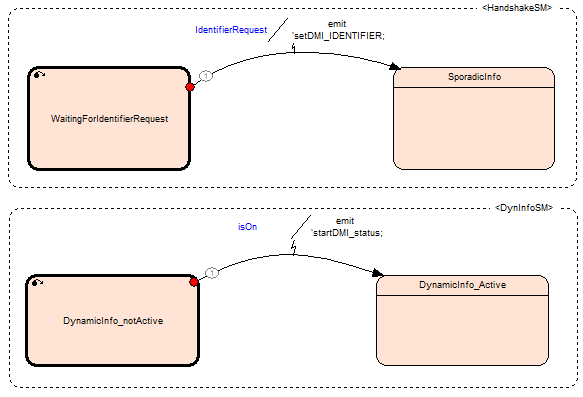
\includegraphics[scale=0.8]{images/DynSporInfoSM}
  \caption{HandshakeSM and DynamicInfoSM State Machines.}
  \label{fig:DynSporSM}
  \end{figure}
  


  With the aim to improve the readability and for a better management of complexity, all the functions (modules, state machines etc.) implemented in each state are divided several diagrams.
  
  The \textit{SporadicInfo} consist of:
  \begin{itemize}
  	\item \textbf{diagram\_SporadicInfo\_Main}: Contains all the modules to manage the sporadic data like ``Enter revalidate Driver ID'', ``Enter or revalidate train running number'', enable buttons in menus. The WindowSM state machine manages the windows that should appear on the DMI(Fig. \ref{fig:win_sm}).
  	
  	\item \textbf{ diagram\_SporadicInfo\_TrainData}: Contains all the logic to store and adapt the incoming train data to a correct visualization on DMI Display.
  	
  	\item \textbf{diagram\_SporadicInfo\_Icon\_Management}: Contains the logic to show/hide one or several icons in area and manage the acknowledgement mechanism if It's required.
  	
  	\item \textbf{ diagram\_SporadicInfo\_DriverID\_TRN}: Contains the logic to store and sent the Train running number and the Driver ID.
  	
  	\item \textbf{diagram\_SporadicInfo\_Text\_Messages}: Contains the modules, state machines and all the logic to manage and display predefined and customized text messages.
  \end{itemize}
  
  The \textit{ DynamicInfo\_Active} state consists of:\\
  
  \begin{itemize}
  	\item \textbf{diagram\_DynamicInfo\_Main}: Contains modules to store and display the informations like the current mode, ETCS level, RBC connection status and location brake target.
  	\item \textbf{diagram\_SpeedSupervision}: Contains the module where are implemented the behaviour of the speed pointer and the circular speed gauge ( informations about speed target, speed permitted and speed release).
  \end{itemize}
  
  \begin{figure}
  	\centering
  	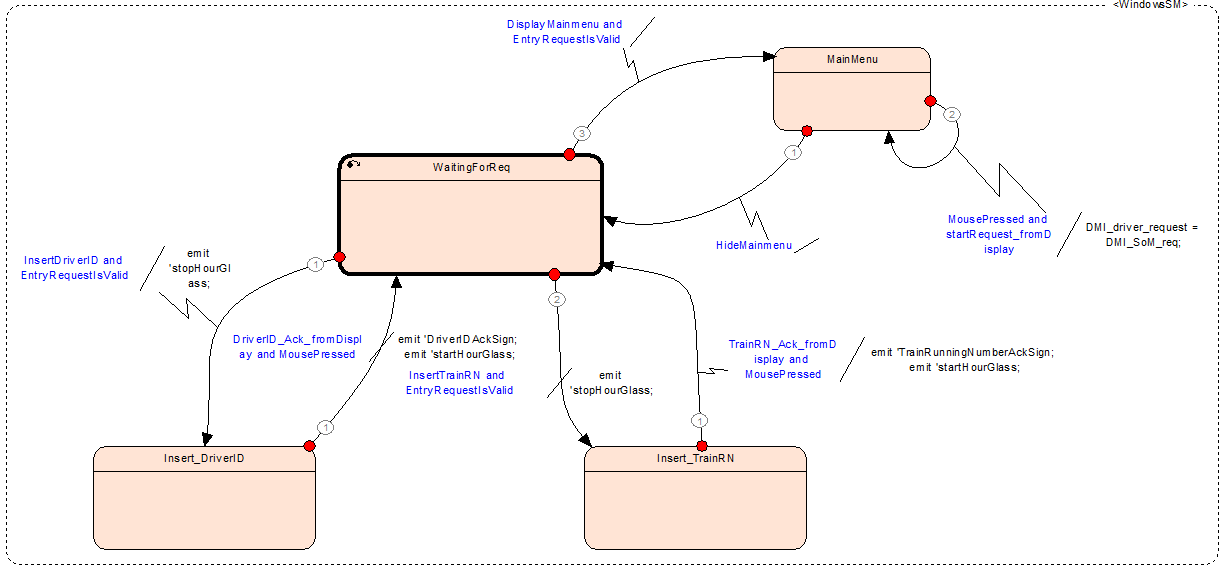
\includegraphics[width=\textwidth]{images/WindowSM}
  	\caption{Windows state machine.}\label{fig:win_sm}
  \end{figure}
  
\paragraph{Communication Protocol}
This section explains which messages are exchanged among DMI Controller, DMI Management and Start of mission procedure. As mentioned previously the DMI Controller is a passive component, It simply responds to requests, therefore is able to cover different scenarios. Below are some examples.
  
  \subparagraph{ Start Of Mission scenario} Are detailed, through a sequence diagram, all the activities (exchanged messages) that should be done to start. In this scenario we have three actors: DMI Controller, DMI Management and SoM procedure (the module where is implemented the start of mission procedure). It's assumed that a OpenDesk signal is received and the system starts in Stand By mode (Fig. \ref{fig:SeqDiaSoM}).
 
  \begin{figure}
  \centering
  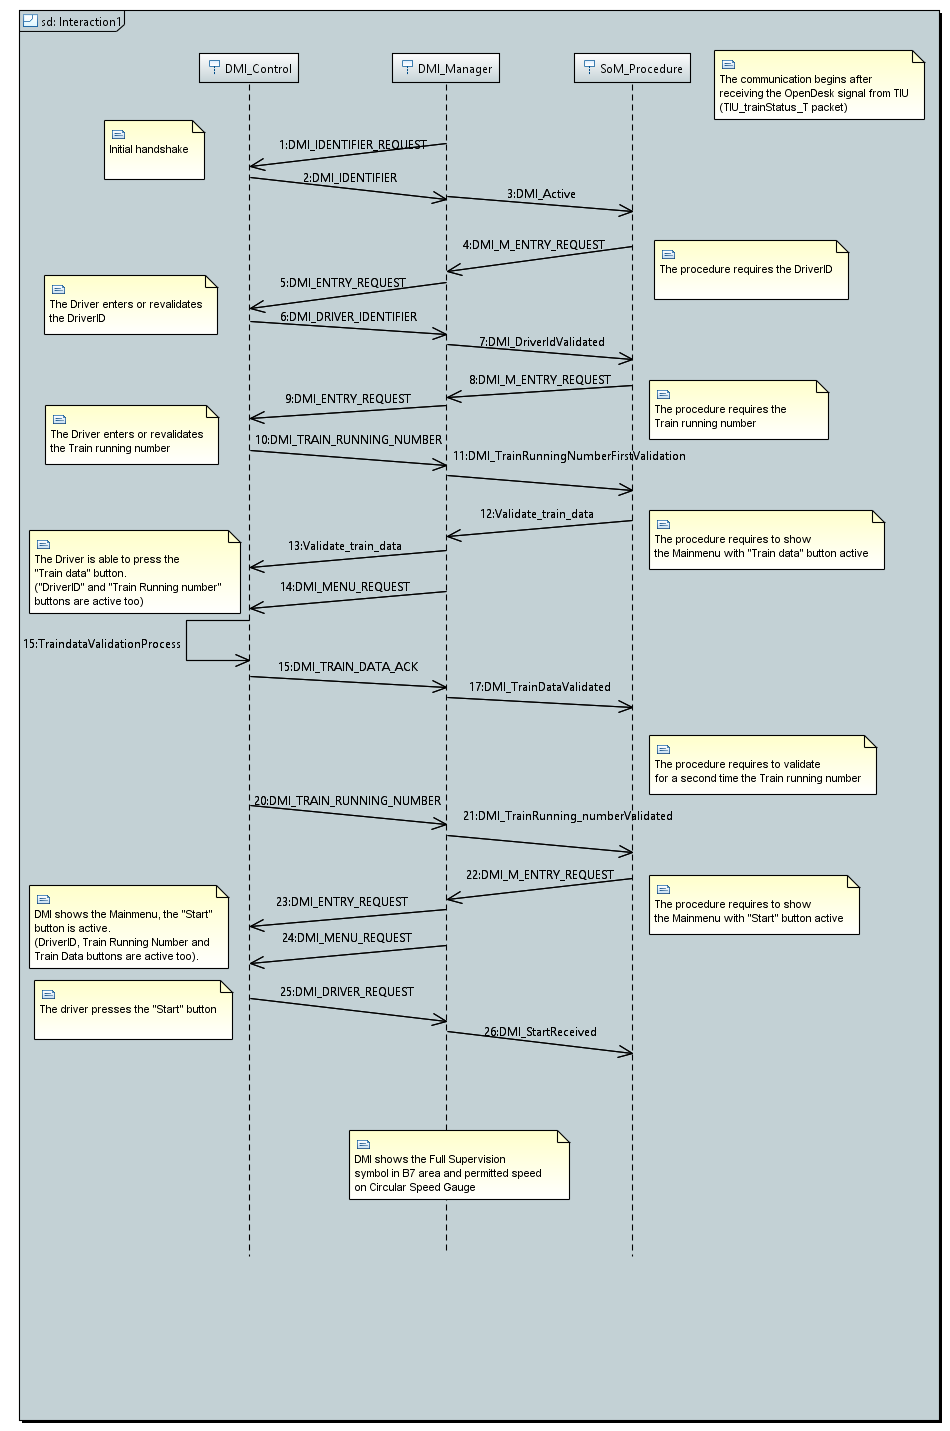
\includegraphics[scale=0.45]{images/SeqDia_DMIctr_DMImng_SoMproc}
  \caption{Sequence Diagram of start of mission scenario}\label{fig:SeqDiaSoM}
  \end{figure}
  

\subparagraph{ Cyclic Exchange of messages}
The time between two messages has not yet been definitively established, It might change in the future. The DMI status packet implements a keep alive mechanism, this means, if the EVC does not receive any DMI status signal during the lapse time, It shall consider a failure in DMI. This check is not yet implemented.

    \begin{figure}
      \centering
      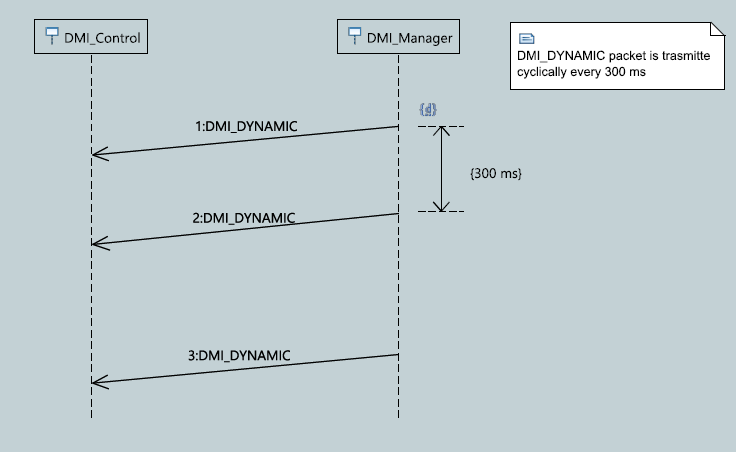
\includegraphics[scale=0.5]{images/DynamicPacket_SeqDia}
      \caption{ Sequence diagram of Dynamic data.}\label{fig:SeqDiaDyn}
    \end{figure}
  
    \begin{figure}
      \centering
      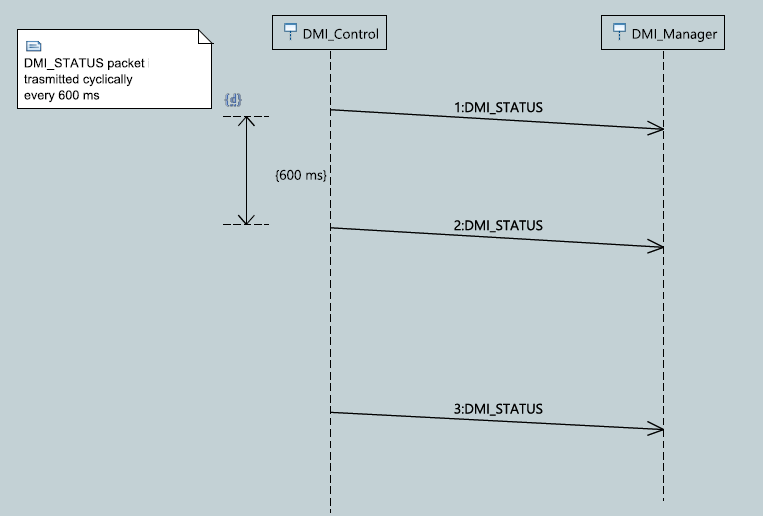
\includegraphics[scale=0.5]{images/DMIStatus_SeqDia}
      \caption{Sequence Diagram of DMI status.}\label{fig:SeqDiaStatus}
     \end{figure}
     

\paragraph{Reference to the Scade Model}

The SCADE model can be found on github under the following path: \url{https://github.com/openETCS/modeling/tree/master/model/Scade/System/DMI_Control}

\bibliographystyle{unsrt}
\bibliography{architecture}


\addcontentsline{toc}{chapter}{Index}
\printindex
%===================================================
%Do NOT change anything below this line

\end{document}
